\chapter{CFG}
\section{Settings}
{\inblue\tt .../jsaf/analysis/cfg/\{package, CFG, CFGId\}.scala}\\
\[
\begin{array}{rllll}
P   & \in & \SF{Program} & = & \powerset{\fid \times \SF{ArgumentsName} \times \args \times \vars} \times \graph \\
fid & \in & \fid & ::= & fid_{global} ~\mid~ fid_1 ~\mid \cdots \\
& & \SF{VarKind} & ::= & \SF{GlobalVar} ~\mid~ \SF{PureLocalVar} ~\mid~ \SF{CapturedVar} ~\mid~ \SF{CapturedCatchVar} \\
& & \args,\vars & ::= & x^* \\
& & \SF{ArgumentsName} & = & \SF{String} \\
G, \langle \controlpoint,\cfgnext,\excnext,\mathbb{A}\rangle & \in & \graph & = & \powerset{\SF{Node}} \times \powerset{\Edge} \times \powerset{\Edge} \times \powerset{\SF{Call}}\\
n & \in & \SF{Node} & = & \fid \times \SF{Label}\\
& & \Edge,\SF{Call} & = & \SF{Node} \times \SF{Node}\\
& & \SF{Label} & ::= & \SF{ENTRY} \mid \SF{EXIT} \mid \SF{EXIT-EXC} \mid c_1 \mid \cdots \\
&&\inblue{\tt Label}&\inblue = &\inblue
{\tt LEntry}\mid {\tt LExit}\mid {\tt LExitExc}\mid {\tt LBlock(id: BlockId)}
\\
\end{array}
\]
  A call expression splits into a pair of call and after-call nodes in this flow graph, and there is no edge between the pair. In order to treat them as a call-site and a return-site of the call, the pair $(cp_{\textit{call}},cp_{\textit{after-call}})$ must be recorded in $\mathbb{A}$ as an element.
\section{Helper Functions}\label{sec:abs-helper}
{\inblue\tt .../jsaf/analysis/cfg/CFG.scala}

\[
\begin{array}{lcl}
  \chf{getCmd}_{P} & : & \SF{Node} \rightarrow \Command \\
  \chf{getArgVars}_{P} & : & \fid \rightarrow \args \\
  \chf{getLocalVars}_{P} & : & \fid \rightarrow \vars \\
  \chf{getCallFromAftercall}_{P} & : & \SF{Node} \rightarrow \SF{Node} \\
  \chf{getAftercallFromCall}_{P} & : & \SF{Node} \rightarrow \SF{Node} \\
  \chf{getExcSucc}_{P} & : & \SF{Node} \rightarrow \SF{Node} \\
  \chf{getArgumentsName}_{P} & : & \fid \rightarrow \SF{String} \\
  \chf{getReturnVar}_{P} & : & \SF{Node} \rightarrow \SF{String} \\
  \chf{getVarKind}_{P} & : & \SF{String} \rightarrow \SF{VarKind} \\
  \chf{isUserFunction}_{P} & : & \SF{FunctionId} \rightarrow \SF{Boolean} \\
\end{array}
\]

\section{Syntax of $\Command$}
{\inblue\tt .../jsaf/analysis/cfg/\{CFG, CFGInst, CFGExpr\}.scala}\\

\[
\begin{array}{r@{~~}r@{~~}lll}
c \in \Command & ::= & \Entry & \mbox{\tt\inblue Entry}& \comment{entry node} \\
& \mid & \Exit & \mbox{\tt\inblue Exit}& \comment{exit node} \\
& \mid & \Exite & \mbox{\tt\inblue ExitExc}& \comment{exit node for exception} \\
& \mid & i^+ & \mbox{\tt\inblue Block}& \comment{basic block} \\

i \in \Instruction & ::= & 
         x~\verb+:=+~\TT{alloc}\verb+(+ e^{?} \verb+)+
 & \mbox{\tt\inblue CFGAlloc}
\\

% & \mid & x~\verb+:=+~\TT{allocObject}\verb+()+
%  & \mbox{\tt\inblue CFGAllocObject}
% \\

& \mid & x~\verb+:=+~\TT{allocArray}\verb+(+n\verb+)+
 & \mbox{\tt\inblue CFGAllocArray}
\\

& \mid & x~\verb+:=+~\TT{allocArg}\verb+(+n\verb+)+
 & \mbox{\tt\inblue CFGAllocArg}
\\

& \mid & x ~\verb+:=+~ e
 & \mbox{\tt\inblue CFGExprStmt}
\\

& \mid & x ~\verb+:=+~ \TT{delete}\verb+(+e\verb+)+
 & \mbox{\tt\inblue CFGDelete}
\\

& \mid & x ~\verb+:=+~ \TT{delete}\verb+(+e_1,e_2\verb+)+
 & \mbox{\tt\inblue CFGDeleteProp}
\\

& \mid & e\verb+[+e\verb+]+ ~\verb+:=+~ e 
 & \mbox{\tt\inblue CFGStore}
\\

%& \mid & \inred \verb+with(+e^*,x,x\verb+)+~\verb+:=+~e
% \\

& \mid & x_1 ~\verb+:=+~ \TT{function} ~x_2^{?}\verb+(+fid\verb+)+
 & \mbox{\tt\inblue CFGFunExpr}
\\

& \mid & \TT{construct}\verb+(+e_1,e_2,e_3\verb+)+
 & \mbox{\tt\inblue CFGConstruct}
\\

& \mid & \TT{call}\verb+(+e_1,e_2,e_3\verb+)+
 & \mbox{\tt\inblue CFGCall}
\\

& \mid & \TT{assert}\verb+(+e\inop e\verb+)+ 
 & \mbox{\tt\inblue CFGAssert}
\\

& \mid & \TT{catch}\verb+(+x\verb+)+
 & \mbox{\tt\inblue CFGCatch}
\\

& \mid & \TT{return}\verb+(+e^{?}\verb+)+ 
 & \mbox{\tt\inblue CFGReturn}
\\

& \mid & \TT{throw}\verb+(+e\verb+)+
 & \mbox{\tt\inblue CFGThrow}
\\

& \mid & x ~\verb+:=+~\ensuremath{\diamond}x\verb+(+x^{*}\verb+)+
 & \mbox{\tt\inblue CFGInternalCall}
\\

& \mid & \TT{noop}
 & \mbox{\tt\inblue CFGNoOp}
\\

e \in \Expression & ::= & x
 & \mbox{\tt\inblue CFGVarRef}
\\

& \mid & e \inop e 
 & \mbox{\tt\inblue CFGBin}
\\

& \mid & \preop e
 & \mbox{\tt\inblue CFGUn}
\\

& \mid & e\verb+[+e\verb+]+
 & \mbox{\tt\inblue CFGLoad}
\\

% & \mid & \inred\verb+with(+e^*,x,x\verb+)+\\
% v \in \Value & ::= 
% & \mid & \inred loc & \inred \comment{Location} \\
& \mid & n & \mbox{\tt\inblue CFGNumber}
&\comment{Number, double}\\
& \mid & ``s" 
 & \mbox{\tt\inblue CFGString}
& \comment{String}\\
& \mid & \TT{true}, \TT{false} 
 & \mbox{\tt\inblue CFGBool}
& \comment{Boolean}\\
& \mid & \TT{null} 
 & \mbox{\tt\inblue CFGNull}
\\
& \mid & \TT{this}
 & \mbox{\tt\inblue CFGThis}
\\
 \preop & ::= &
\multicolumn{3}{l}{
 \TT{void} \mid \TT{typeof} \mid \TT{+} \mid \TT{-} \mid \TT{\~} \mid \TT{!}} \\
 \inop & ::= &
\multicolumn{3}{l}{
 \TT{instanceof} \mid \TT{in} \mid \TT{|} \mid \TT{\&}
               \mid \TT{\^} \mid \TT{<<} \mid \TT{>>} \mid \TT{>>>}
\mid \TT{+} \mid \TT{-} \mid \TT{*} \mid \TT{/} \mid \TT{\%} \mid \TT{==} \mid \TT{!=} 
\mid \TT{===}} \\
&\mid& \TT{!==} \mid \TT{<} \mid \TT{>} \mid \TT{<=} \mid \TT{>=}

\end{array}
\]

\chapter{IR to CFG}
This section describes the \safe translation rules from IR to CFG,
whose implementation is available at:
\begin{verbatim}
$SAFE_HOME/src/main/scala/kr/ac/kaist/safe/cfg_builder/
           CFGBuilder.scala
\end{verbatim}

\noindent
$
\begin{array}{l@{~~}l}
\LabelMap &: \JSLabel \mapsto \powerset{\CFGBlock}\\
\JSLabel &= \RetLabel \mid \ThrowLabel \mid \ThrowEndLabel \\
& \ \ \mid \AfterCatchLabel \mid \UserLabel\\
\UserLabel &= \String\\
\end{array}
$

\[
\begin{array}{l@{~~}l}
\transfun{-}_{\emph{root}} &: \IRRoot \rightarrow \CFG \\
\transfun{-}_{\emph{fdvars}} &: \IRFunDecl^{*} \rightarrow \CFGId^{*} \\
\transfun{-}_{\emph{vds}} &: \IRVarStmt^{*} \rightarrow \CFGId^{*} \\
\transfun{-}_{\emph{args}} &: \IRStmt^{*} \rightarrow \CFGId^{*} \\
\transfun{-}_{\emph{functional}} &: \IRFunctional \rightarrow \CFGFunction \\
\transfun{-}_{\emph{fd}} &: \IRFunDecl \times \CFGFunction \times \NormalBlock \rightarrow \Unit \\
\transfun{-}_{\emph{fd}^{*}} &: \IRFunDecl^{*} \times \CFGFunction \times \NormalBlock \rightarrow \Unit \\
\transfun{-}_{\emph{stmt}} &: \IRStmt \times \CFGFunction \times \CFGBlock^{*} \times \LabelMap\\
& \rightarrow \CFGBlock^{*} \times \LabelMap\\
\transfun{-}_{\emph{stmt}^{*}} &: \IRStmt^{*} \times \CFGFunction \times \CFGBlock^{*} \times \LabelMap\\
& \rightarrow \CFGBlock^{*} \times \LabelMap\\
\transfun{-}_{\emph{mem}} &: \IRField \times \NormalBlock \times \IRId \rightarrow \Unit \\
\transfun{-}_{\emph{elem}} &: \IRExpr \times \NormalBlock \times \IRId \times \Integer \rightarrow \Unit \\
\transfun{-}_{\emph{expr}} &: \IRExpr \rightarrow \CFGExpr \\
\transfun{-}_{\emph{id}} &: \IRId \rightarrow \CFGId \\
\end{array}
\]

We use the following global variables for describing the translation from IR to CFG:
\[
\begin{array}{lll}
*\ \emph{catchVars} &: \powerset{\String} & \text{ initialized to } \emptyset\\
*\ \emph{cfg} &: \CFG &\\
*\ \emph{cfgIdMap} &: \String \mapsto \CFGId & \text{ initialized to } [\ ]\\
*\ \emph{currentFunc} &: \CFGFunction & \\
\end{array}
\]

\[
\begin{array}{l@{}l@{~}l}
\lefteqn{\transfun{\IRRoot(\emph{fds}, \emph{vds}, \emph{stmts})}_{\emph{root}}}\\
& = & \emph{globalVars} \letval \transfun{\emph{fds}}_{\emph{fdvars}} ~\emph{++}~ \transfun{\emph{vds}}_{\emph{vds}} \\
& & \emph{cfg} \leftarrow \new\ \CFG(\emph{globalVars})\\
& & \emph{globalFunc} \letval \emph{cfg}.\emph{globalFunc}\\
& & \emph{currentFunc} \leftarrow \emph{globalFunc}\\
& & \emph{startBlock} \letval \emph{globalFunc}.\emph{createBlock}\\
& & \emph{cfg}.\emph{addEdge}(\emph{globalFunc}.\emph{entry}, \emph{startBlock})\\
& & \transfun{\emph{fds}}_{\emph{fd}^*}(\emph{globalFunc}, \emph{startBlock})\\
& & (B, L) \letval \transfun{\emph{stmts}}_{\emph{stmt}^{*}}(\emph{globalFunc}, \emph{startBlock}, [\ ])\\
& & \emph{cfg}.\emph{addEdge}(B, \emph{globalFunc}.\emph{exit})\\
& & \emph{cfg}.\emph{addEdge}(L(\TT{ThrowLabel}), \emph{globalFunc}.\emph{exitExc}, \EdgeExc)\\
& & \emph{cfg}.\emph{addEdge}(L(\TT{ThrowEndLabel}), \emph{globalFunc}.\emph{exitExc})\\
& & \emph{cfg}.\emph{addEdge}(L(\TT{AfterCatchLabel}), \emph{globalFunc}.\emph{exitExc})\\
& & \emph{cfg}\\
& & \\
\lefteqn{\transfun{\emph{fds}}_{\emph{fdvars}}}\\
 & = &
\fold(\emph{fds})(\Nil)(\lambda(\emph{vars}, \irfundeclsmall{f}{\_}{\_}{\_}{\_}{\_}{\_} \Rightarrow \emph{vars} :: \transfun{f}_{\emph{id}})\\
& & \\

\lefteqn{\transfun{\emph{vds}}_{\emph{vds}}}\\
 & = &
\fold(\emph{vds})(\Nil)(\lambda(\emph{vars}, \irvar{x})\Rightarrow \emph{vars} :: \transfun{x}_{\emph{id}})\\
& & \\

\lefteqn{\transfun{\emph{args}}_{\emph{args}}}\\
 & = &
\fold(\emph{args})(\Nil)(\lambda(\emph{args}, x = \emph{arguments}[i]) \Rightarrow \emph{args} :: \transfun{x}_{\emph{id}})\\
& & \\
\lefteqn{\transfun{\irfunctionalsmall{\_}{\emph{name}}{\emph{params}}{\emph{args}}{\emph{fds}}{\emph{vds}}{\emph{body}}}_{\emph{functional}}}\\
& = & \emph{argVars} \letval \transfun{\emph{args}}_{\emph{args}}\\
& & \emph{localVars} \letval \transfun{\emph{fds}}_{\emph{fdvars}} \emph{++} \transfun{\emph{vds}}_{\emph{vds}}\\
& & \emph{argumentsName} \letval \headOf(\emph{params}).\emph{name}\\
& & \emph{nameStr} \letval \emph{name}.\emph{name}\\
& & \emph{newFunc} \letval \emph{cfg}.\emph{createFunction}(\emph{argumentsName}, \emph{argVars},\\
& & \emph{localVars}, \emph{nameStr})\\
& & \emph{oldFunc} \letval \emph{currentFunc}\\
& & \emph{currentFunc} \leftarrow \emph{newFunc}\\
& & \emph{startBlock} \letval \emph{newFunc}.\emph{createBlock}\\
& & \emph{cfg}.\emph{addEdge}(\emph{newFunc}.\emph{entry}, \emph{startBlock})\\
& & \transfun{\emph{fds}}_{\emph{fd}^{*}}(\emph{newFunc}, \emph{startBlock})\\
& & (B, L) \letval \transfun{\emph{body}}_{\emph{stmt}^{*}}(\emph{newFunc}, \emph{startBlock}, [\ ])\\
& & \emph{cfg}.\emph{addEdge}(B, \emph{newFunc}.\emph{exit})\\
& & \emph{cfg}.\emph{addEdge}(L(\TT{RetLabel}), \emph{newFunc}.\emph{exit})\\
& & \emph{cfg}.\emph{addEdge}(L(\TT{ThrowLabel}), \emph{newFunc}.\emph{exitExc}, \EdgeExc)\\
& & \emph{cfg}.\emph{addEdge}(L(\TT{ThrowEndLabel}), \emph{newFunc}.\emph{exitExc})\\
& & \emph{cfg}.\emph{addEdge}(L(\TT{AfterCatchLabel}), \emph{newFunc}.\emph{exitExc})\\
& & \emph{currentFunc} \leftarrow \emph{oldFunc}\\
& & \emph{newFunc}\\
& & \\

\lefteqn{\transfun{\IRFunDecl(\emph{functional})}_{\emph{fd}}(\emph{func}, \emph{block})}\\
& = & \emph{lhs} \letval \transfun{\emph{functional}.\emph{name}}_{\emph{id}}\\
& & \emph{newFunc} \letval \transfun{\emph{functional}}_{\emph{functional}}\\
& & (\emph{addr1}, \emph{addr2}) \letval (\new\ \Address,\ \new\ \Address)\\
& & \emph{block}.\emph{createInst}(\emph{lhs} := \TT{function}\ (\emph{newFunc}) ~@~
\TT{(}\emph{addr1},\ \emph{addr2}\TT{)})\\
& & \\

\lefteqn{\transfun{\emph{fds}}_{\emph{fd}^{*}}(\emph{func}, \emph{block})}\\
& = & \iter(\emph{fds})(\lambda(\emph{fd}) \Rightarrow \transfun{fd}_{\emph{fd}}(\emph{func}, \emph{block}))\\
& & \\

\end{array}
\]

\[
\begin{array}{l@{}l@{~}l}
\lefteqn{\transfun{\irstmtunit{\emph{stmts}}}_{\emph{stmt}}(f, B, L)}\\
 & = &
\transfun{\emph{stmts}}_{\emph{stmt}^{*}}(f, B, L)\\
& & \\

\lefteqn{\transfun{\irseq{\emph{stmts}}}_{\emph{stmt}}(f, B, L)}\\
 & = &
\transfun{\emph{stmts}}_{\emph{stmt}^{*}}(f, B, L)\\
& & \\

\lefteqn{\transfun{\SF{IRFunExpr}(\emph{lhs}, \emph{functional})}_{\emph{stmt}}(f, B, L)}\\
& = & \emph{newFunc} \letval \transfun{\emph{functional}}_{\emph{functional}}\\
& & (\emph{addr1}, \emph{addr2}, \emph{addr3}) \letval (\new\ \Address,\ \new\ \Address,\\
& & \phantom{(\emph{addr1}, \emph{addr2}, \emph{addr3}) \letval (}\new\ \Address)\\
& & \emph{name} \letval \transfun{\emph{functional}.\emph{name}}_{\emph{id}}\\
& & \emph{tailBlock} \letval \getTail(B, f)\\
& & if\ (\emph{name}.\emph{kind} = \TT{CapturedVar}) \\
& & \phantom{if} \emph{tailBlock}.\emph{createInst}(\emph{lhs} := \TT{function}\ \emph{name}\ (\emph{newFunc}) \\
& & \phantom{if \emph{tailBlock}.\emph{createInst}(\emph{lhs} :=}
~@~ \TT{(}\emph{addr1},\ \emph{addr2}, \emph{addr3}\TT{)})\\
& & else\\
& & \phantom{if} \emph{tailBlock}.\emph{createInst}(\emph{lhs} := \TT{function}\ (\emph{newFunc}) ~@~
\TT{(} \emph{addr1},\\
& & \phantom{if \emph{tailBlock}.\emph{createInst}(\emph{lhs} := \TT{function}\ (\emph{newFunc}) ~@~ \TT{(}}\emph{addr2}\TT{)})\\
& & (\emph{tailBlock}, L)\\
& & \\

\lefteqn{\transfun{\irobject{x}{\emph{members}}}_{\emph{stmt}}(f, B, L)}\\
& = & \emph{tailBlock} \letval \getTail(B, f)\\
& & \emph{addr1} \letval \new\ \Address\\
& & \emph{tailBlock}.\emph{createInst}(x := \TT{alloc}() ~@~ \emph{addr1})\\
& & iter(\emph{members})(\lambda(m) \Rightarrow \transfun{m}_{\emph{mem}}(tailBlock, x))\\
& & (\emph{tailBlock}, L[\ThrowLabel \mapsto \emph{tailBlock} \cup L(\ThrowLabel)])\\
& & \\

\lefteqn{\transfun{\irobject{x}{\emph{members}, \emph{proto}}}_{\emph{stmt}}(f, B, L)}\\
& = & \emph{tailBlock} \letval \getTail(B, f)\\
& & \emph{protoId} \letval \transfun{\emph{proto}}_{\emph{expr}}\\
& & \emph{addr1} \letval \new\ \Address\\
& & \emph{tailBlock}.\emph{createInst}(x := \TT{alloc}(\emph{protoId}) ~@~ \emph{addr1})\\
& & iter(\emph{members})(\lambda(m) \Rightarrow \transfun{m}_{\emph{mem}}(tailBlock, x))\\
& & (\emph{tailBlock}, L[\ThrowLabel \mapsto \emph{tailBlock} \cup L(\ThrowLabel)])\\
& & \\

\lefteqn{\transfun{\ircfgtrycat{\emph{body}}{x}{\emph{catIR}}}_{\emph{stmt}}(f, B, L)}\\
& = & \emph{catchVars} \leftarrow \emph{catchVars} \cup \{ x.\emph{name} \}\\
& & \emph{tryB} \letval f.\emph{createBlock}\\
& & \emph{cfg}.\emph{addEdge}(B, \emph{tryB})\\
& & \emph{catB} \letval f.\emph{createBlock}\\
& & \emph{catB}.\emph{createInst}(\TT{catch}(\transfun{x}_{\emph{id}}))\\
& & (\emph{trybs}, \emph{trylmap}) \letval \transfun{\emph{body}}_{\emph{stmt}}(f, \emph{tryB}, [\ ])\\
& & \emph{cfg}.\emph{addEdge}(\emph{trylmap}(\ThrowLabel), \emph{catB}, \EdgeExc)\\
& & \emph{cfg}.\emph{addEdge}(\emph{trylmap}(\ThrowEndLabel), \emph{catB})\\
& & \emph{cfg}.\emph{addEdge}(\emph{trylmap}(\AfterCatchLabel), \emph{catB})\\
& & \emph{tmplmap} \letval \emph{trylmap} - \ThrowLabel - \ThrowEndLabel\\
&& \phantom{\emph{tmplmap} \letval} - \AfterCatchLabel\\
& & (\emph{catchbs}, \emph{catchlamp}) \letval \transfun{\emph{catIR}}_{\emph{stmt}}(f, \emph{catB}, \emph{tmplmap})\\
& & (\emph{trybs} ~\emph{++}~ \emph{catchbs}, L ~\emph{++}~ \emph{catchlmap})\\
\end{array}
\]

\[
\begin{array}{l@{}l@{~}l}
\lefteqn{\transfun{\ircfgtryfin{\emph{body}}{\emph{finIR}}}_{\emph{stmt}}(f, B, L)}\\
& = & \emph{tryB} \letval f.\emph{createBlock}\\
& & \emph{cfg}.\emph{addEdge}(B, \emph{tryB})\\
& & \emph{finB} \letval f.\emph{createBlock}\\
& & (\emph{trybs}, \emph{trylmap}) \letval \transfun{\emph{body}}_{\emph{stmt}}(f, \emph{tryB}, [\ ])\\
& & (\emph{finbs}, \emph{finlamp}) \letval \transfun{\emph{finIR}}_{\emph{stmt}}(f, \emph{finB}, L)\\
& & \emph{cfg}.\emph{addEdge}(\emph{trybs}, \emph{finB})\\
& & \emph{reslmap} \letval \fold(\emph{trylmap} - \AfterCatchLabel)\\
& & \phantom{\emph{reslmap} \letval \fold}(\emph{finlmap})
(\lambda((l, B'), L') \Rightarrow \\
& & \quad \emph{dupB} \letval f.\emph{createBlock}\\
& & \quad (B'', L'') \letval \transfun{\emph{finIR}}_{\emph{stmt}}(f, \emph{dupB}, L')\\
& & \quad if\ (l = \ThrowLabel)\\
& & \quad \phantom{if} \emph{cfg}.\emph{addEdge}(\emph{trylmap}(\AfterCatchLabel),\ \emph{dupB})\\
& & \quad \phantom{if} \emph{cfg}.\emph{addEdge}(B', \emph{dupB}, \EdgeExc)\\
& & \quad \phantom{if} L''[\ThrowEndLabel \mapsto (L''(\ThrowEndLabel) ~\emph{++}~ B'')]
~~~~~~~~~~~~~~~~\\
& & \quad else\\
& & \quad \phantom{if} \emph{cfg}.\emph{addEdge}(B', \emph{dupB}, \EdgeExc)\\
& & \quad \phantom{if} L''[l \mapsto (L''(l) ~\emph{++}~ B'')]\\
& & )\\
& & (\emph{finbs}, \emph{reslmap})\\
& & \\

\lefteqn{\transfun{\irtryfull{\emph{body}}{x}{\emph{catIR}}{\emph{finIR}}}_{\emph{stmt}}(f, B, L)}\\
& = & \emph{catchVars} \leftarrow \emph{catchVars} \cup \{ x.\emph{name} \}\\
& & \emph{tryB} \letval f.\emph{createBlock}\\
& & \emph{cfg}.\emph{addEdge}(B, \emph{tryB})\\
& & \emph{catB} \letval f.\emph{createBlock}\\
& & \emph{catB}.\emph{createInst}(\TT{catch}(\transfun{x}_{\emph{id}}))\\
& & \emph{finB} \letval f.\emph{createBlock}\\
& & (\emph{trybs}, \emph{trylmap}) \letval \transfun{\emph{body}}_{\emph{stmt}}(f, \emph{tryB}, [\ ])\\
& & \emph{cfg}.\emph{addEdge}(\emph{trylmap}(\ThrowLabel), \emph{catB}, \EdgeExc)\\
& & \emph{cfg}.\emph{addEdge}(\emph{trylmap}(\ThrowEndLabel), \emph{catB})\\
& & \emph{cfg}.\emph{addEdge}(\emph{trylmap}(\AfterCatchLabel), \emph{catB})\\
& & \emph{tmplmap} \letval \emph{trylmap} - \ThrowLabel - \ThrowEndLabel\\
&& \phantom{\emph{tmplmap} \letval} - \AfterCatchLabel\\
& & (\emph{catchbs}, \emph{catchlamp}) \letval \transfun{\emph{catIR}}_{\emph{stmt}}(f, \emph{catB}, \emph{tmplmap})\\
& & (\emph{finbs}, \emph{finlamp}) \letval \transfun{\emph{finIR}}_{\emph{stmt}}(f, \emph{finB}, L)\\
& & \emph{cfg}.\emph{addEdge}(\emph{trybs} ~\emph{++}~ \emph{catchbs}, \emph{finB})\\
& & \emph{reslmap} \letval \fold(\emph{catchlmap} - \AfterCatchLabel)\\
& & \phantom{\emph{reslmap} \letval \fold}(\emph{finlmap})
(\lambda((l, B'), L') \Rightarrow \\
& & \quad \emph{dupB} \letval f.\emph{createBlock}\\
& & \quad (B'', L'') \letval \transfun{\emph{finIR}}_{\emph{stmt}}(f, \emph{dupB}, L')\\
& & \quad if\ (l = \ThrowLabel)\\
& & \quad \phantom{if} \emph{cfg}.\emph{addEdge}(\emph{catchlmap}(\AfterCatchLabel), \emph{dupB})\\
& & \quad \phantom{if} \emph{cfg}.\emph{addEdge}(B', \emph{dupB}, \EdgeExc)\\
& & \quad \phantom{if} L''[\ThrowEndLabel \mapsto (L''(\ThrowEndLabel) ~\emph{++}~ B'')]\\
& & \quad else\\
& & \quad \phantom{if} \emph{cfg}.\emph{addEdge}(B', \emph{dupB}, \EdgeExc)\\
& & \quad \phantom{if} L''[l \mapsto (L''(l) ~\emph{++}~ B'')]\\
& & )\\
& & (\emph{finbs}, \emph{reslmap})\\
& & \\
\end{array}
\]

\[
\begin{array}{l@{}l@{~}l}
\lefteqn{\transfun{\irarray{x}{\emph{elems}}}_{\emph{stmt}}(f, B, L)\qquad \mbox{for \mtt{IRArgs}}}\\
& = & \emph{tailBlock} \letval \getTail(B, f)\\
& & \emph{addr} \letval \new\ \Address\\
& & \emph{tailBlock}.\emph{createInst}(x := \TT{allocArg}(\length(\emph{elems})) ~@~ \emph{addr})\\
& & \iter(\emph{elems})(0)(\lambda(e,k) \Rightarrow \transfun{e}_{\emph{elem}}(\emph{tailBlock}, x, k))\\
& & (\emph{tailBlock}, L[\ThrowLabel \mapsto L(\ThrowLabel) \cup \{ \emph{tailBlock} \})\\
& & \\

\lefteqn{\transfun{\irarray{x}{\emph{elems}}}_{\emph{stmt}}(f, B, L)\qquad \mbox{for \mtt{IRArray}}}\\
& = & \emph{tailBlock} \letval \getTail(B, f)\\
& & \emph{addr} \letval \new\ \Address\\
& & \emph{tailBlock}.\emph{createInst}(x :=\TT{allocArray}(\length(\emph{elems})) ~@~ \emph{addr})\\
& & \iter(\emph{elems})(0)(\lambda(e,k) \Rightarrow \transfun{e}_{\emph{elem}}(\emph{tailBlock}, x, k))\\
& & (\emph{tailBlock}, L[\ThrowLabel \mapsto L(\ThrowLabel) \cup \{ \emph{tailBlock} \})\\
& & \\

% TODO IRInternalCall

\lefteqn{\transfun{\ircfgcall{x}{\emph{fun}}{\emph{thisB}, \emph{args}}}_{\emph{stmt}}(f, B, L)}\\
& = & \emph{tailBlock} \letval \getTail(B, f)\\
& & \emph{this} \letval \mbox{a CFG local variable of name \TT{"<>this<>"}}\\
& & \emph{tailBlock}.\emph{createInst}(\emph{this} := \TT{enterCode}(\transfun{\emph{thisB}}_{\emph{expr}}))\\
& & (\emph{addr1}, \emph{addr2}) \letval (\new\ \Address,\ \new\ \Address)\\
& & \emph{call} \letval \emph{tailBlock}.\emph{func}.\emph{createCall}(\TT{call}(\transfun{\emph{fun}}_{\emph{expr}}, \emph{this}, \transfun{\emph{args}}_{\emph{expr}})\\
&& \phantom{\emph{call} \letval }
 ~@~ \TT{(}\emph{addr1},\ \emph{addr2}\TT{)}, \transfun{x}_{\emph{id}})\\
& & \emph{cfg}.\emph{addEdge}(\emph{tailBlock}, \emph{call})\\
& & (\emph{call}.\emph{afterCall}, L[\\
& & \quad \ThrowLabel \mapsto L(\ThrowLabel) \cup \{ \emph{call}, \emph{tailBlock} \},\\
& & \quad \AfterCatchLabel \mapsto L(\AfterCatchLabel)\\
& & \quad \phantom{\AfterCatchLabel \mapsto} \cup \{ \emph{call}.\emph{afterCatch} \}\\
& & ])\\

\lefteqn{\transfun{{\sf break}\ \emph{label}}_{\emph{stmt}}(f, B, L)}\\
& = & \emph{key} \letval \emph{label}.\emph{name}\\
& & \emph{bs} \letval L(\emph{key}) \cup B\\
& & (\emptyset, L[\emph{key} \mapsto \emph{bs}])\\
& & \\

\lefteqn{\transfun{\ircfgnew{x_1}{{\sf new}\ x_2}{\emph{args}}}_{\emph{stmt}}(f, B, L)}\\
& = & \emph{tailBlock} \letval \getTail(B, f)\\
& & (\emph{addr1}, \emph{addr2}) \letval (\new\ \Address,\ \new\ \Address) \\
& & \emph{call} \letval \emph{tailBlock}.\emph{func}.\emph{createCall}(\\
& & \quad \TT{construct}(\transfun{x_2}_{\emph{expr}}, \transfun{\emph{args}(0)}_{\emph{expr}}, \transfun{\emph{args}(1)}_{\emph{expr}})\\
& & \phantom{\quad }
@~ \TT{(}\emph{addr1}, \emph{addr2}\TT{)}, \transfun{x_1}_{\emph{id}}\\
& & )\\
& & \emph{cfg}.\emph{addEdge}(\emph{tailBlock}, \emph{call})\\
& & (\emph{call}.\emph{afterCall}, L[\\
& & \quad \ThrowLabel \mapsto L(\ThrowLabel) \cup \{ \emph{call}, \emph{tailBlock} \},\\
& & \quad \AfterCatchLabel \mapsto L(\AfterCatchLabel)\\
& & \phantom{\quad \AfterCatchLabel \mapsto}
\cup \{ \emph{call}.\emph{afterCatch} \}\\
& & ])\\
& & \\

\lefteqn{\transfun{\irdelete{x}{e}}_{\emph{stmt}}(f, B, L)}\\
& = & \emph{tailBlock} \letval \getTail(B, f)\\
& & \emph{tailBlock}.\emph{createInst}(\transfun{x}_{\emph{id}} := \TT{delete}(\transfun{e}_{\emph{expr}}))\\
& & (\emph{tailBlock}, L[\ThrowLabel \mapsto L(\ThrowLabel) \cup \{ \emph{tailBlock} \}])\\
& & \\

\lefteqn{\transfun{\irdeleteobj{x}{e_1}{e_2}}_{\emph{stmt}}(f, B, L)}\\
& = & \emph{tailBlock} \letval \getTail(B, f)\\
& & \emph{tailBlock}.\emph{createInst}(\transfun{x}_{\emph{id}} := \TT{delete}(\transfun{e_1}_{\emph{expr}}, \transfun{e_2}_{\emph{expr}}))\\
& & (\emph{tailBlock}, L[\ThrowLabel \mapsto L(\ThrowLabel) \cup \{ \emph{tailBlock} \}])\\
& & \\

\end{array}
\]

\[
\begin{array}{l@{}l@{~}l}
\lefteqn{\transfun{\ircfgexpr{x}{e}}_{\emph{stmt}}(f, B, L)}\\
& = & \emph{tailBlock} \letval \getTail(B, f)\\
& & \emph{tailBlock}.\emph{createInst}(\transfun{x}_{\emph{id}} := \transfun{e}_{\emph{expr}})\\
& & (\emph{tailBlock}, L[\ThrowLabel \mapsto L(\ThrowLabel) \cup \{ \emph{tailBlock} \}])\\
& & \\

\lefteqn{\transfun{\ircfgif{\emph{cond}}{\emph{trueIR}}}_{\emph{stmt}}(f, B, L)}\\
& = & \emph{trueB} \letval f.\emph{createBlock}\\
& & \emph{cfg}.\emph{addEdge}(B, \emph{trueB})\\
& & \emph{falseB} \letval f.\emph{createBlock}\\
& & \emph{cfg}.\emph{addEdge}(B, \emph{falseB})\\
& & \emph{cfgCond} \letval \transfun{\emph{cond}}_{\emph{expr}}\\
& & \emph{trueB}.\emph{createInst}(\TT{assert}(\emph{cfgCond}))\\
& & \emph{falseB}.\emph{createInst}(\TT{assert}(\neg \emph{cfgCond}))\\
& & (B', L') \letval \transfun{\emph{trueIR}}_{\emph{stmt}}(f, trueB, L)\\
& & \emph{endB} \letval f.\emph{createBlock}\\
& & \emph{cfg}.\emph{addEdge}(\{ \emph{falseB},\ B' \}, \emph{endB})\\
& & (\emph{endB}, L'[\ThrowLabel \mapsto L'(\ThrowLabel)\\
& & \phantom{(\emph{endB}, L'[\ThrowLabel \mapsto}
 \cup \{ \emph{trueB},\ \emph{falseB} \}])\\

\lefteqn{\transfun{\irifelse{\emph{cond}}{\emph{trueIR}}{\emph{falseIR}}}_{\emph{stmt}}(f, B, L)}\\
& = & \emph{trueB} \letval f.\emph{createBlock}\\
& & \emph{cfg}.\emph{addEdge}(B, \emph{trueB})\\
& & \emph{falseB} \letval f.\emph{createBlock}\\
& & \emph{cfg}.\emph{addEdge}(B, \emph{falseB})\\
& & \emph{cfgCond} \letval \transfun{\emph{cond}}_{\emph{expr}}\\
& & \emph{trueB}.\emph{createInst}(\TT{assert}(\emph{cfgCond}))\\
& & \emph{falseB}.\emph{createInst}(\TT{assert}(\neg \emph{cfgCond}))\\
& & (B', L') \letval \transfun{\emph{trueIR}}_{\emph{stmt}}(f, trueB, L)\\
& & \emph{endB} \letval f.\emph{createBlock}\\
& & (B'', L'') \letval \transfun{\emph{falseIR}}_{\emph{stmt}}(f, falseB, L')\\
& & \emph{cfg}.\emph{addEdge}(B' ~\emph{++}~ B'', \emph{endB})\\
& & (\emph{endB}, L''[\ThrowLabel \mapsto L''(\ThrowLabel)\\
& & \phantom{(\emph{endB}, L''[\ThrowLabel \mapsto}
\cup \{ \emph{trueB},\ \emph{falseB} \}])\\
& & \\

\lefteqn{\transfun{\irlabel{l}{s}}_{\emph{stmt}}(f, B, L)}\\
& = & b \letval f.\emph{createBlock}\\
& & (B', L') \letval \transfun{s}_{\emph{stmt}}(f, B, L)\\
& & \emph{label} \letval l.\emph{name}\\
& & \emph{cfg}.\emph{addEdge}(B', b)\\
& & \emph{cfg}.\emph{addEdge}(L'(\emph{label}), b)\\
& & (b, L' - l)\\
& & \\

\lefteqn{\transfun{\mbox{\sf return}}_{\emph{stmt}}(f, B, L)}\\
& = & \emph{tailBlock} \letval \getTail(B, f)\\
& & \emph{tailBlock}.\emph{createInst}(\TT{return}())\\
& & (\emptyset, L[\RetLabel \mapsto L(\RetLabel) \cup \{ \emph{tailBlock}\}])\\
& & \\

\lefteqn{\transfun{\ircfgreturn{e}}_{\emph{stmt}}(f, B, L)}\\
& = & \emph{tailBlock} \letval \getTail(B, f)\\
& & \emph{tailBlock}.\emph{createInst}(\TT{return}(\transfun{e}_{\emph{expr}}))\\
& & (\emptyset, L[\RetLabel \mapsto L(\RetLabel) \cup \{ \emph{tailBlock}\}])\\
& & \\

\lefteqn{\transfun{\irstore{x_1}{x_2}{e}}_{\emph{stmt}}(f, B, L)}\\
& = & \emph{tailBlock} \letval \getTail(B, f)\\
& & \emph{tailBlock}.\emph{createInst}(\transfun{x_1}_{\emph{expr}}[\transfun{x_2}_{\emph{expr}}] := \transfun{e}_{\emph{expr}})\\
& & (\emph{tailBlock}, L[\ThrowLabel \mapsto L(\ThrowLabel) \cup \{ \emph{tailBlock} \}])\\
\end{array}
\]

\[
\begin{array}{l@{}l@{~}l}
\lefteqn{\transfun{\irthrow{e}}_{\emph{stmt}}(f, B, L)}\\
& = & \emph{tailBlock} \letval \getTail(B, f)\\
& & \emph{tailBlock}.\emph{createInst}(\TT{throw}(\transfun{e}_{\emph{expr}}))\\
& & (\emptyset, L[\ThrowLabel \mapsto L(\ThrowLabel) \cup \{ \emph{tailBlock} \}])\\
\\

\lefteqn{\transfun{\ircfgwhile{e}{s}}_{\emph{stmt}}(f, B, L)}\\
& = & \emph{tailBlock} \letval \getTail(B, f)\\
& & \emph{head} \letval f.\emph{createBlock}\\
& & \emph{body} \letval f.\emph{createBlock}\\
& & \emph{out} \letval f.\emph{createBlock}\\
& & \emph{cfgCond} \letval \transfun{\emph{e}}_{\emph{expr}}\\
& & \emph{body}.createInst(\TT{assert}(\emph{cfgCond}))\\
& & \emph{out}.createInst(\TT{assert}(\neg \emph{cfgCond}))\\
& & \emph{cfg}.\emph{addEdge}(\emph{tailBlock}, \emph{head})\\
& & \emph{cfg}.\emph{addEdge}(\emph{head}, \emph{body})\\
& & \emph{cfg}.\emph{addEdge}(\emph{head}, \emph{out})\\
& & (B', L') \letval \transfun{s}_{\emph{stmt}}(f, [\emph{body}], L)\\
& & \emph{cfg}.\emph{addEdge}(B', \emph{head})\\
& & (\emph{out}, L'[\ThrowLabel \mapsto L'(\ThrowLabel)\\
& & \phantom{(\emph{out}, L'[\ThrowLabel \mapsto } \cup \{ \emph{body},\ \emph{out} \}]) \\
& & \\

\lefteqn{\transfun{\emph{stmts}}_{\emph{stmt}^{*}}(f, B, L)}\\
& = & \fold(\emph{stmts})((B, L))(\lambda((B', L'), \emph{stmt}) \Rightarrow\\
&& \phantom{\fold(\emph{stmts})((B, L))(} \transfun{\emph{stmt}}_{\emph{stmt}}(f, B', L'))\\
& & \\

\lefteqn{\transfun{\emph{mem}}_{\emph{mem}}(b, x)}\\
& = & \emph{lhs} \letval \transfun{x}_{\emph{expr}}\\
& & \emph{str} \letval \emph{mem}.\emph{prop}.\emph{name}\\
& & \emph{expr} \letval \transfun{\emph{mem}.\emph{expr}}_{\emph{expr}}\\
& & b.\emph{createInst}(\emph{lhs}[\emph{str}] := \emph{expr})\\
& & \\

\lefteqn{\transfun{e}_{\emph{elem}}(b, x, k)}\\
& = & \emph{lhs} \letval \transfun{x}_{\emph{expr}}\\
& & \emph{expr} \letval \transfun{e}_{\emph{expr}}\\
& & b.\emph{createInst}(\emph{lhs} [``k"] := \emph{expr})\\
& & \\

\transfun{x}_{\emph{expr}} & = & x\\
& & \\

\transfun{e_1 \inop e_2}_{\emph{expr}}
& = & \transfun{e_1}_{\emph{expr}} \inop \transfun{e_2}_{\emph{expr}}\\
& & \\

\transfun{\preop e}_{\emph{expr}}
& = & \preop \transfun{e}_{\emph{expr}}\\
& & \\

\transfun{x [e]}_{\emph{expr}}
 & = & \transfun{x}_{\emph{expr}} [ \transfun{e}_{\emph{expr}} ]\\
& & \\

\transfun{\this}_{\emph{expr}} & = & \this\\
& & \\

\transfun{v}_{\emph{expr}} & = & v\\
& & \\

\transfun{x}_{\emph{id}}
& = & \text{let }\emph{kind} \text{ be a } \VarKind \text{ based on the information}\\
& & \text{from } \TT{CapturedVariableCollector}\\
& & \new\ \CFGId(x.\emph{name}, \emph{kind})\\
\end{array}
\]

%\newpage

\chapter{CFG Collecting Semantics}
 Assumptions and limitations are as follows:
\begin{itemize}
\item All the variables declared by `\TT{var}' are included in the set $\vars$.
\item Followings are not yet supported: regular expression, with, getter, setter, eval.
\item Runtime exception is omitted. \TT{throw} is the only way to make an exception.
\item Semantics of operators are omitted.
\item Semantics for helper functions is not written using denotational semantics(they are not compositional).
\item Try-catch clause in a finally block can disturb a flow of a previous throwed value.
\end{itemize}

\section{Settings}
\[
\begin{array}{rlcl}
x \in & \SF{Prop} & =  & \SF{String} \cup
                       \set{
                         \varprop{return},\ \varprop{exception},\ \varprop{exception\_all},\ \varprop{this},\
                         \varprop{up},\ \varprop{outer} \\
                         \varprop{proto},\ \varprop{scope},\ \varprop{class},\
                         \varprop{function},\ \varprop{extensible},\ \varprop{construct}
                       }\\
l \in & \SF{Loc}  & ::= & %\varloc{temp} ~\mid~
               \varloc{Global}
               ~\mid~ \varloc{ObjProto}
               ~\mid~ \varloc{ArrayProto}
               ~\mid~ \varloc{RefErrProto} \\
&&             \mid & \varloc{RangeErrProto}
               ~\mid~ \varloc{TypeErrProto}\\

&     & \mid  & l_1 ~\mid~ \cdots \\
cp \in & \SF{ControlPoint} & = & \SF{Node} \\
H \in & \SF{Heap} & =  & \SF{Loc} \finto \SF{Obj} \\
o \in & \SF{Obj}  & =  & \SF{Prop} \finto \SF{PropValue} \\
A \in & \SF{Env} & = & \SF{Loc}\listd \\
(H,A), \SF{stuck} \in & \SF{State} & = & \SF{Heap} \times \SF{Env} \\
      & \SF{PropValue} & = & \SF{ObjectValue} \cup \SF{Value} \cup \fid \cup \SF{Env} \\
      &       &    & \inblue \textit{`$\SF{Value}\cup \fid\cup \SF{Env}$' is for internal property.} \\
v \in & \SF{Value} & = & \SF{Loc} \cup \SF{PValue} \\
ov \in& \SF{ObjectValue} & = & \set{
                                   value: \SF{Value}; \\
                                   writable: \SF{Bool}; \\
                                   enumerable: \SF{Bool}; \\
                                   configurable: \SF{Bool}; \\
                                 } \\
pv\in & \SF{PValue}& = & \SF{Number}
                     \cup \SF{String}
                     \cup \SF{Bool}
                     \cup \set{\SF{undefined},\ \SF{null}} \\
n \in & \SF{Number} & ::= & \SF{NaN} ~\mid~ \SF{Inf} ~\mid~ -\SF{Inf} ~\mid~ 0 ~\mid~ 1 ~\mid~ -1 ~\mid~ 2 ~\mid~\cdots\\
s \in & \SF{String}\\
b \in & \SF{Bool} \\
exc \in & \SF{Exception} & ::= & \exc{ReferenceError} ~\mid~ \exc{RangeError} ~\mid~ \exc{TypeError}
\end{array}
\]

\section{Helper Functions}
\[
\begin{array}{ll}
& \chf{PushStack}(l_o^*,l_n) = l_n::l_o^* \\
& \chf{TopStack}(l_n::l_o^*) = l_n \\\\
& \chf{Dom}(H) = \set{l\ |\ l\mapsto o \in H} \\
& \chf{Dom}(o) = \set{x\ |\ x\mapsto v \in o} \\
\\
& \chf{IsArray}(H,l) = \left\{
  \begin{array}{l@{\quad\quad\quad}l}
    \vtrue &\ifc{H(l)(\varprop{class}) =
  ``Array"}\\
    \vfalse &\owc\\
  \end{array}\right.
\\
& \chf{IsObject}(H,l) = \left\{
  \begin{array}{l@{\quad\quad\quad}l}
    \vtrue &\ifc{H(l)(\varprop{class}) =
  ``Object"\lor H(l)(\varprop{class}) = ``Function"}\\
    \vfalse &\owc\\
  \end{array}\right.
\\\\
\chf{IsArrayIndex} & : \SF{Value} \rightarrow \SF{Bool} \\
& \chf{IsArrayIndex}(v)
  = 
  \left\{
    \begin{array}{l@{\quad\quad}l}
      \vtrue & \ifc{\chf{toString}(\chf{\inred ToUint32}(\chf{toString}(v))) = \chf{toString}(v)\\
        \land\ \chf{\inred ToUint32}(\chf{toString}(v)) \neq 2^{32}-1} \\
      \vfalse & \owc\\
    \end{array}
  \right.
\\
\\

\chf{VarStore} & : \SF{Heap} \times \SF{Env} \times \SF{Prop} \times \SF{Value}
\times \SF{Bool} \rightarrow \SF{Heap} \\
& \chf{VarStore}(H,[\varloc{Global}], x, v, b)
  =  \chf{PropStore}(H,\varloc{Global},x,v) \\
& \quad\ifc{x\not\in\chf{Dom}(H(\varloc{Global}))} \\
& \chf{VarStore}(H,l_{hd}::l_{tl}^{*},x,v,b)
  =  H[l_{hd}\mapsto H(l_{hd})[x\mapsto \set{H(l_{hd})(x) \rwith value=v; writable=b}]]\\
& \quad\ifc{x \in \chf{Dom}(H(l_{hd}))}\\
& \chf{VarStore}(H,l_{hd}::l_{tl}^{*},x,v,b)
  =  \chf{VarStore}(H,l_{tl}^{*},x,v,b)\\
& \quad\ifc{x \not\in \chf{Dom}(H(l_{hd}))}\\\\

\chf{VarStoreE} & : \SF{Heap} \times \SF{Env} \times \SF{Prop} \times \SF{Value}
\times \SF{Bool} \rightarrow \SF{Heap} \\
& \chf{VarStoreE}(H,A, t, v, b) = \chf{VarStore}(H,A, t, v, b) \\
& \chf{VarStoreE}(H,A, x, v, b) = \left\{
  \begin{array}{ll}
    \chf{VarStore}(H,A, x, v, b) &\ifc{\chf{CanPutVar}(H,A,x)}\\
    H & \owc
  \end{array}
\right. \\\\

\chf{PropStore} & : \SF{Heap} \times \SF{Loc} \times \SF{Prop} \times \SF{Value} \rightarrow \SF{Heap} \\
& \chf{PropStore}(H,l,x,v)
  = H\left[l\mapsto H(l)\left[x\mapsto \set{
    value=v;\\
   enumerable=\vtrue;\\
    configurable=\vtrue;\\
    writable=\vtrue
 }\right]\right]\\
& \quad\ifc{x\not\in \chf{Dom}(H(l))} \\
& \chf{PropStore}(H,l,x,v)
  = H\left[l\mapsto H(l)\left[x\mapsto \set{H(l)(x)\rwith value=v}\right]\right]\\
& \quad\ifc{x\in \chf{Dom}(H(l))} \\

\\
\chf{Delete} & : \SF{Heap} \times \SF{Loc} \times \SF{Prop} \rightarrow \SF{Heap}
\times \SF{Bool}\\
& \chf{Delete}(H,l,x)
  =  (H,\vtrue)\\
& \quad\ifc{\lnot\chf{HasOwnProperty}(H,l,x)} \\
& \chf{Delete}(H,l,x)
  =  (H,\vfalse)\\
& \quad\ifc{\chf{HasOwnProperty}(H,l,x)\land
    H(l)(x).configurable = \vfalse} \\
& \chf{Delete}(H,l,x)
  =  (H[l\mapsto H(l) - x],\vtrue)\\
& \quad\ifc{\chf{HasOwnProperty}(H,l,x) \land H(l)(x).configurable = \vtrue} \\\\

\chf{Lookup} & : \SF{Heap} \times \SF{Env} \times \SF{Prop} \rightarrow \SF{Value} \cup \SF{Exception}\\

&
\begin{array}{ll}
% Exception
% & \chf{Lookup}(H,[\varloc{Global}],x)
%   =  \exc{ReferenceError} \quad\ifc{\lnot\chf{HasProperty}(H,\varloc{Global},x)} \\

  \chf{Lookup}(H,[\varloc{Global}],x)
  =  \exc{ReferenceError} & \ifc{\lnot\chf{HasProperty}(H,\varloc{Global},x)} \\
  \chf{Lookup}(H,[\varloc{Global}],x)
  =  \chf{Proto}(H, \varloc{Global}, x) & \ifc{\chf{HasProperty}(H,\varloc{Global},x)}\\
% & \chf{Lookup}(H,l_{hd}::l_{tl}^{*},x)
%   =  \exc{RefError} \quad\ifc{H(l_{hd})(x).value = \bot} \\
  \chf{Lookup}(H,l_{hd}::l_{tl}^{*},x)
   =  H(l_{hd})(x).value & \ifc{x\in\chf{Dom}(H(l_{hd}))} \\
   \chf{Lookup}(H,l_{hd}::l_{tl}^{*},x)
   =  \chf{Lookup}(H, l_{tl}^{*},x) & \ifc{x\not\in\chf{Dom}(H(l_{hd}))}\\
\end{array}\\
\\
\end{array}
\]
\[
\begin{array}{ll}
\chf{TypeTag} & : \SF{Heap} \times \SF{Value} \rightarrow \set{``number", ``string", ``boolean", ``object",\\ ``function", ``null", ``undefined"}\\
& \chf{TypeTag}(H,v) = \left\{
\begin{array}{l@{\quad\quad}l}
  ``number" & \ifc{v \in \SF{Number}} \\
  ``boolean" & \ifc{v \in \SF{Boolean}} \\
  ``string" & \ifc{v \in \SF{String}} \\
  ``object" & \ifc{v \in \SF{Loc}\land\lnot\chf{IsCallable}(H,v)} \\
  ``function" & \ifc{v \in \SF{Loc}\land\chf{IsCallable}(H,v)} \\
  ``object" & \ifc{v = \SF{null}} \\
  ``undefined" & \ifc{v = \SF{undefined}} \\
\end{array}
\right. \\
\\

\chf{CanPut} & : \SF{Heap} \times \SF{Loc} \times \SF{Prop} \rightarrow \SF{Bool}\\
&
\begin{array}{ll}
  \chf{CanPut}(H,l,x) = \chf{CanPutHelp}(H,l,x,l) & \\
\end{array}
\\\\

\chf{CanPutHelp} & : \SF{Heap} \times \SF{Loc} \times \SF{Prop} \times \SF{Loc}
\rightarrow \SF{Bool}\\
&
\begin{array}{ll}
  \chf{CanPutHelp}(H,l_1,x,l_2) = \chf{CanPutHelp}(H,H(l_1)(\varprop{proto}).value,x,l_2) &\\
   \quad\ifc{x\not\in\chf{Dom}(H(l_1)) \land H(l_1)(\varprop{proto}).value\ \neq \SF{null}}&\\
  \chf{CanPutHelp}(H,l_1,x,l_2) = H(l)(\varprop{extensible}) &\\
  \quad\ifc{x\not\in\chf{Dom}(H(l_1)) \land H(l_1)(\varprop{proto}).value\ = \SF{null}}&\\
  \chf{CanPutHelp}(H,l_1,x,l_2) = H(l_1)(x).writable &\\
  \quad\ifc{x\in\chf{Dom}(H(l_1))}&\\
\end{array}
\\\\

\chf{CanPutVar} & : \SF{Heap} \times \SF{Env} \times \SF{Prop} \rightarrow \SF{Bool}\\
&
\begin{array}{ll}
  \chf{CanPutVar}(H,[\varloc{Global}],x)
  =  \chf{CanPut}(H,\varloc{Global},x) \\
\chf{CanPutVar}(H,l_{hd}::l^{*}_{tl},x)
  =  H(l_{hd})(x).writable & \ifc{x\in\chf{Dom}(H(l_{hd}))} \\
\chf{CanPutVar}(H,l_{hd}::l^{*}_{tl},x)
  =  \chf{CanPutVar}(H,l^{*}_{tl},x) & \ifc{x\not\in\chf{Dom}(H(l_{hd}))} \\
\end{array}\\
\\

\chf{HasProperty} & : \SF{Heap} \times \SF{Loc} \times \SF{Prop} \rightarrow \SF{Bool} \\
& \chf{HasProperty}(H,l,x) = \vtrue \\
& \quad\ifc{\chf{HasOwnProperty}(H,l,x)} \\
& \chf{HasProperty}(H,l,x) = \vfalse \\
& \quad\ifc{\lnot\chf{HasOwnProperty}(H,l,x) \land H(l_1)(\varprop{proto}).value\ = \SF{null}}\\
& \chf{HasProperty}(H,l,x) = \chf{HasProperty}(H,H(l)(\varprop{proto}).value,x)\\
& \quad\ifc{\lnot\chf{HasOwnProperty}(H,l,x) \land H(l_1)(\varprop{proto}).value\ \neq \SF{null}} \\
\\
\\

\chf{HasOwnProperty} & : \SF{Heap} \times \SF{Loc} \times \SF{Prop} \rightarrow \SF{Bool} \\
&
\begin{array}{ll}
  \chf{HasOwnProperty}(H,l,x) = \vfalse & \ifc{x\not\in\chf{Dom}(H(l))} \\
  \chf{HasOwnProperty}(H,l,x) = \vtrue & \ifc{x\in\chf{Dom}(H(l))} \\
\end{array}\\
\\
\chf{LookupBase} & : \SF{Heap} \times \SF{Env} \times \SF{Prop} \rightarrow \SF{Loc} \\
&
\begin{array}{ll}
\chf{LookupBase}(H,[\varloc{Global}],x)
= \chf{ProtoBase}(H, \varloc{Global}, x) \\
\chf{LookupBase}(H,l_{hd}::l_{tl}^{*},x)
= l_{hd} & \ifc{x\in\chf{Dom}(H(l_{hd}))} \\
\chf{LookupBase}(H,l_{hd}::l_{tl}^{*},x)
= \chf{LookupBase}(H, l_{tl}^{*},x) & \ifc{x\not\in\chf{Dom}(H(l_{hd}))} \\
\end{array}\\
\\
\end{array}
\]
\[
\begin{array}{ll}
\chf{ProtoBase} & : \SF{Heap} \times \SF{Loc} \times \SF{Prop} \rightarrow \SF{Loc}\\
& 
\begin{array}{ll}
  \chf{ProtoBase}(H,l,x) = l &\\
    \quad\ifc{x\in\chf{Dom}(H(l))}&\\
  \chf{ProtoBase}(H,l,x) = \{ \} &\\
    \quad\ifc{x\not\in\chf{Dom}(H(l)) \land H(l)(\varprop{proto}).value\ = \SF{null}}&\\
  \chf{ProtoBase}(H,l,x) =  \chf{ProtoBase}(H,H(l)(\varprop{proto}).value,x) &\\
    \quad\ifc{x\not\in\chf{Dom}(H(l)) \land H(l)(\varprop{proto}).value\ \neq \SF{null}}&\\
\end{array}\\
\\
\chf{Proto} & : \SF{Heap} \times \SF{Loc} \times \SF{Prop} \rightarrow \SF{Value}\\
& 
\begin{array}{ll}
  \chf{Proto}(H,l,x) =  H(l)(x).value &\\
    \quad\ifc{x\in\chf{Dom}(H(l))}&\\
  \chf{Proto}(H,l,x) =  \chf{Proto}(H,H(l)(\varprop{proto}).value,x) &\\
    \quad\ifc{ x\not\in\chf{Dom}(H(l)) \land H(l)(\varprop{proto}).value\ \neq \SF{null}}\\
  \chf{Proto}(H,l,x) = \SF{undefined} &\\
    \quad\ifc{ x\not\in\chf{Dom}(H(l)) \land H(l)(\varprop{proto}).value\ = \SF{null}}\\
\end{array}\\
\\
\chf{NewObject} & : \SF{Loc} \rightarrow \SF{Obj} \\
& \chf{NewObject}(l) = \set{\varprop{class}\mapsto "Object",\\
  \varprop{proto}\mapsto
  \set{
    value=l;\\writable=\vfalse;\\
    enumerable=\vfalse;\\configurable=\vfalse\\
    },\\
  \varprop{extensible}\mapsto \vtrue}\\\\

\chf{NewFunctionObject} & : \fid \times \SF{Env} \times \SF{Loc} \times \SF{Number} \rightarrow \SF{Obj} \\
& \chf{NewFunctionObject}(fid,A,l,n) = \set{
    \varprop{class}\mapsto ``Function",\\
    \varprop{function}\mapsto fid,\\
    \varprop{construct}\mapsto fid,\\
    \varprop{scope}\mapsto A,\\
    \varprop{proto}\mapsto
    \set{
      value=\varloc{FunctionProto};\\writable=\vfalse;\\
      enumerable=\vfalse;\\configurable=\vfalse
    },\\
    ``prototype"\mapsto \set{
        value:l;\\
        writable:\vtrue;\\
        enumerable:\vfalse;\\
        configurable:\vfalse
      },\\
    ``length"\mapsto \set{
        value:n;\\
        writable:\vfalse;\\
        enumerable:\vfalse;\\
        configurable:\vfalse
      },\\
    \varprop{extensible}\mapsto \vtrue
}\\\\
\chf{NewArrayObject} & : \SF{Number} \rightarrow \SF{Obj} \\
& \chf{NewArrayObject}(n) = \set{
    \varprop{class}\mapsto ``Array",\\
    \varprop{proto}\mapsto 
    \set{
      value=\varloc{ArrayProto};\\writable=\vfalse;\\
      enumerable=\vfalse;\\configurable=\vfalse
    },\\
   ``length"\mapsto \set{
       value:n;\\
       writable:\vtrue;\\
       enumerable:\vfalse;\\
       configurable:\vfalse
     },\\
    \varprop{extensible}\mapsto \vtrue
}\\\\

\end{array}
\]
\[
\begin{array}{ll}

\chf{NewArgObject} & : \SF{Number} \rightarrow \SF{Obj} \\
& \chf{NewArgObject}(n) = \set{
    \varprop{class}\mapsto ``Arguments",\\
    \varprop{proto}\mapsto 
    \set{
      value=\varloc{ObjProto};\\writable=\vfalse;\\
      enumerable=\vfalse;\\configurable=\vfalse
    },\\
   ``length"\mapsto \set{
       value:n;\\
       writable:\vtrue;\\
       enumerable:\vfalse;\\
       configurable:\vtrue
     },\\
    \varprop{extensible}\mapsto \vtrue
}\\\\

\chf{NewBoolean} & : \SF{Bool} \rightarrow \SF{Obj} \\
& \chf{NewBoolean}(v) = \set{
    \varprop{class}\mapsto ``Boolean",\\
    \varprop{proto}\mapsto 
    \set{
      value=\varloc{BoolProto};\\writable=\vfalse;\\
      enumerable=\vfalse;\\configurable=\vfalse
    },\\
    \varprop{extensible}\mapsto \vtrue, \\
    \varprop{primitive}\mapsto v
}\\\\

\chf{NewNumber} & : \SF{Number} \rightarrow \SF{Obj} \\
& \chf{NewNumber}(v) = \set{
    \varprop{class}\mapsto ``Number",\\
    \varprop{proto}\mapsto 
    \set{
      value=\varloc{NumProto};\\writable=\vfalse;\\
      enumerable=\vfalse;\\configurable=\vfalse
    },\\
    \varprop{extensible}\mapsto \vtrue, \\
    \varprop{primitive}\mapsto v
}\\\\

\chf{NewString} & : \SF{String} \rightarrow \SF{Obj} \\
& \chf{NewString}(s) = o_1 \cup o_2 \\
& \quad\wherec{
  v_{len} = length(s)\\
  \land\ o_1 = \set{
    \varprop{class}\mapsto ``String",\\
    \varprop{proto}\mapsto 
    \set{
      value=\varloc{StrProto};\\writable=\vfalse;\\
      enumerable=\vfalse;\\configurable=\vfalse
    },\\
    \varprop{extensible}\mapsto \vtrue, \\
    \varprop{primitive}\mapsto s, \\
    ``length"\mapsto \set{
      value=v_{len};\\writable=\vfalse;\\
      enumerable=\vfalse;\\configurable=\vfalse
    }
  }\\
  \land\ o_2 = \set{\left.``i"\mapsto \set{
      value = v_{char};\\writable=\vfalse;\\
      enumerable=\vtrue;\\configurable=\vfalse
    } ~\right|~ 0 \leq i < v_{len}\land\ v_{char}=charAt(s,i)}
}\\\\

\chf{IsCallable} & : \SF{Heap} \times \SF{Loc} \rightarrow \SF{Bool} \\
& \chf{IsCallable}(H,l)
  = \left\{
    \begin{array}{l@{\quad\quad\quad}l}
      \vtrue &\ifc{\varprop{function}\in\chf{Dom}(H(l))}\\
      \vfalse &\owc
    \end{array}
    \right.\\\\
\end{array}
\]
\[
\begin{array}{ll}
\chf{HasConstruct} & : \SF{Heap} \times \SF{Loc} \rightarrow \SF{Bool} \\
& \chf{HasConstruct}(H,l)
  = \left\{
    \begin{array}{l@{\quad\quad\quad}l}
      \vtrue & \ifc{\varprop{construct}\in\chf{Dom}(H(l))}\\
      \vfalse &\owc
    \end{array}
    \right.\\\\

\chf{newLocation} & : \SF{Unit} \rightarrow \SF{Loc} \\
& \chf{newLocation}()
  = l_{new}\\
\\
\chf{toNumber} & : \SF{PValue} \rightarrow \SF{Number} \\
& \chf{toNumber}(pv)
  = 
  \left\{
    \begin{array}{l@{\quad\quad}l}
      \SF{NaN} & \ifc{pv=\SF{undefined}} \\
      \SF{0}   & \ifc{pv=\SF{null}\lor pv=\vfalse} \\
      \SF{1}   & \ifc{pv=\vtrue} \\
      pv   & \ifc{pv\in\SF{Number}} \\
      \inred \chf{Str2Num}(pv)   & \ifc{pv\in\SF{String}} \\
    \end{array}
  \right.\\
\\
\chf{toString} & : \SF{PValue} \rightarrow \SF{String} \\
& \chf{toString}(pv)
  = 
  \left\{
    \begin{array}{l@{\quad\quad}l}
      ``undefined" & \ifc{pv=\SF{undefined}} \\
      ``null"      & \ifc{pv=\SF{null}} \\
      ``pv"        & \ifc{pv\in\SF{Boolean}} \\
      ``\SF{$pv$}" & \ifc{pv\in\SF{Number}} \\
      pv           & \ifc{pv\in\SF{String}} \\
    \end{array}
  \right.\\
\\
\chf{toBoolean} & : \SF{Value} \rightarrow \SF{Bool} \\
& \chf{toBoolean}(v)
  = 
  \left\{
    \begin{array}{l@{\quad\quad}l}
      \vfalse   & \ifc{v=\SF{undefined}} \\
      \vfalse   & \ifc{v=\SF{null}} \\
      v         & \ifc{v\in\SF{Boolean}} \\
      \vfalse   & \ifc{v\in\SF{Number}\land v\in\set{\sf 0,NaN}} \\
      \vtrue    & \ifc{v\in\SF{Number}\land v\not\in\set{\sf 0,NaN}} \\
      \vfalse   & \ifc{v\in\SF{String}\land v=``"} \\
      \vtrue    & \ifc{v\in\SF{String}\land v\neq``"} \\
      \vtrue    & \ifc{v\in\SF{Loc}}
    \end{array}
  \right.\\
\\
\chf{toPrimitive} & : \SF{Value} \rightarrow \SF{PValue} \\
& \chf{toPrimitive}(v)
  = 
  \left\{
    \begin{array}{l@{\quad\quad}l}
      v & \ifc{v\not\in\SF{Loc}} \\
      \inred \chf{Obj2Str}(v)   & \ifc{v\in\SF{Loc}} \\
    \end{array}
  \right.\\
\\
\chf{toObject} & : \SF{Heap} \times \SF{Value} \rightarrow \SF{Heap} \times \SF{Value} \cup \SF{Exception}\\
& \chf{toObject}(H, l) = (H, l)\\
& \chf{toObject}(H, v) = (H, \SF{TypeError}) \quad\ifc{v \in \set{\SF{undefined}, \SF{null}}}\\
& \chf{toObject}(H, v) = (H_1, l_{new}) \\
& \quad\wherec{
  o = \left\{
    \begin{array}{ll}
      \chf{NewString}(v) & \ifc{v \in \SF{String}}\\
      \chf{NewNumber}(v) & \ifc{v \in \SF{Number}}\\
      \chf{NewBoolean}(v) & \ifc{v \in \SF{Bool}}\\
    \end{array}
  \right. \\
  H_1 = H[l_{new}\mapsto o] \\
  l_{new} = \chf{newLocation}()
}\\
\\
\end{array}
\]
\[
\begin{array}{ll}
\chf{getThis} & : \SF{Value} \rightarrow \SF{Loc} \\
& \chf{getThis}(v)
  = 
  \left\{
    \begin{array}{l@{\quad\quad}l}
      \varloc{Global} & \ifc{v=\SF{undefined}} \\
      \varloc{Global} & \ifc{v=\SF{null}} \\
      \varloc{Global} & \ifc{v\in\SF{Loc} \land \lnot\chf{IsObject}(v)} \\
      v               & \ifc{v\in\SF{Loc} \land \chf{IsObject}(v)}\\
    \end{array}
  \right.\\
\\
\chf{inherit} & : \SF{Heap} \times \SF{Loc} \times \SF{Loc} \rightarrow \SF{Value} \\
& \chf{inherit}(H,l_1,l_2) = \left\{
  \begin{array}{ll}
    \vtrue & \ifc{l_1 = l_2} \\
    \vfalse & \ifc{l_1 \neq l_2 \land H(l_1)(\varprop{proto}).value\ = \SF{null}} \\
    \chf{inherit}(H,H(l_1)(\varprop{proto}).value,l_2) & \ifc{l_1 \neq l_2 \land H(l_1)(\varprop{proto}).value\ \neq \SF{null}} \\
  \end{array}
  \right.\\
\\
\chf{iteratorInit} & : \SF{Obj} \times \powerset{\SF{Prop}} \times \SF{Number} \rightarrow \SF{Obj} \\
& \chf{iteratorInit}(o,P,n) = 
  \left\{
  \begin{array}{l}
    \{\varprop{i}\mapsto 0\} \\\quad\ifc{P = \emptyset} \\
    \chf{iteratorInit}(o,P-x,n+1)[n\mapsto x] \\\quad \ifc{x\in P} \\
  \end{array}
  \right.\\
\\
\chf{collectProps} & : \SF{Heap} \times \SF{Loc} \rightarrow \powerset{\SF{Loc}} \\
& \chf{collectProps}(H,l) = 
  \left\{
  \begin{array}{ll}
    \chf{Dom}(H(l)) \cup\ \chf{CollectProps}(H,H(l)(\varprop{proto}).value)
    & \ifc{H(l)(\varprop{proto}).value \neq \SF{null}} \\
    \{\} & \ifc{H(l)(\varprop{proto}).value = \SF{null}} \\
  \end{array}
  \right.\\
\\
\end{array}
\]
\[
\begin{array}{ll}
\chf{isEnumerable} & : \SF{Heap} \times \SF{Loc} \times \SF{Prop} \rightarrow \SF{Bool} \\
& \chf{isEnumerable}(H,l,x) =
  \left\{
    \begin{array}{l}
      H(l)(x).enumerable \\
      \quad\ifc{x\in\chf{Dom}(H(l))} \\
      \chf{isEnumerable}(H,H(l)(\varprop{proto}).value,x) \\
      \quad\ifc{x\notin\chf{Dom}(H(l)) \land H(l)(\varprop{proto}).value \neq \SF{null}} \\
      \vfalse \\
      \quad\ifc{x\notin\chf{Dom}(H(l)) \land H(l)(\varprop{proto}).value = \SF{null}} \\
    \end{array}
  \right.\\
\\
\chf{next} & : \SF{Heap} \times \SF{Obj} \times \SF{Number} \times \SF{Loc} \rightarrow \SF{Number} \\
& \chf{next}(H,o_{iter},n,l) = 
  \left\{
  \begin{array}{ll}
    n &\ifc{n\notin \chf{Dom}(o_{iter})} \\
    n &\ifc{n\in \chf{Dom}(o_{iter})
%      \land\ \chf{HasProperty}(H,l,o_{iter}(n))\\
      \land\ \chf{isEnumerable}(H,l,o_{iter}(n))} \\
    \chf{next}(H,o_{iter},n+1,l) & \owc\\
  \end{array}
  \right.\\
\\
\chf{NewExceptionObject} & : \SF{Exception} \rightarrow \SF{Obj} \\
& \chf{NewExceptionObject}(exc) = \chf{NewObject}(l)\\
& \quad\wherec{
  l=\left\{
    \begin{array}{ll}
      \varloc{RefErrProto}&\ifc{exc = \exc{ReferenceError}} \\
      \varloc{RangeErrProto}&\ifc{exc = \exc{RangeError}} \\
      \varloc{TypeErrProto}&\ifc{exc = \exc{TypeError}} \\
    \end{array}
  \right.
}\\\\
\chf{RaiseException} & : \SF{Heap} \times \SF{Exception}\cup\SF{Value} \rightarrow \SF{Heap} \\
& \chf{RaiseException}(H,v) = H_1 \\
& \quad\wherec{
  H_1 = H[\varloc{temp}\mapsto H(\varloc{temp})[\varprop{exception}\mapsto v]]
}\\
& \chf{RaiseException}(H,exc) = H_2 \\
& \quad\wherec{
  l_e = \chf{newLocation}() \\
  H_1 = H[l_e\mapsto\chf{NewExceptionObject}(exc)] \\
  H_2 = H_1[\varloc{temp}\mapsto H_1(\varloc{temp})[\varprop{exception}\mapsto l_{e}]]
}
\end{array}
\]
% \[
% \begin{array}{ll}
% \chf{@ToObject} & : \SF{PValue} \rightarrow \SF{} \\
% & \chf{Prim2Str}(v)
% \end{array}
% \]

\newpage
\section{Semantics}
\[
\begin{array}{lcl}
  \N & \in & \SF{ControlPoint} \rightarrow \Command \rightarrow \powerset{\SF{State}} \rightarrow \powerset{\SF{State}} \\
  \I & \in & \SF{ControlPoint} \rightarrow \SF{Instruction} \rightarrow \SF{State} \rightarrow \SF{State} \\
  \V & \in & \SF{Expression} \rightarrow \SF{State} \rightarrow \SF{Value} \cup \SF{Exception}\\
  \B & \in & \SF{Expression} \rightarrow \SF{State} \rightarrow \SF{State} \\
\end{array}
\]
\[
\begin{array}{l} 
% \Entry & \comment{entry node}\\\\
\N _{cp}\lbr {\sf entry} \rbr S = 
 \bigcup\set{(H_1,A) \mid (H,A)\in S} \\
 \quad\wherec{
   ({fid_{this}},\SF{ENTRY}) = cp \land l=\chf{TopStack}(A)\\
   \land\ x_{argvar}^{*} = \chf{getArgVars}_P({fid_{this}})\ 
   \land\ x_{localvar}^{*} = \chf{getLocalVars}_P({fid_{this}}) \\
   \land\ H_1=H\left[l\mapsto
   H(l)
     \left[
       \begin{array}{l}
         \left(x_{argvar}\mapsto\set{value=\SF{undefined};writable=\vtrue;\\
             enumerable=\vfalse;configurable=\vfalse}\right)^{*}, \\
         \left(x_{localvar}\mapsto\set{value=\SF{undefined};writable=\vtrue;\\
             enumerable=\vtrue;configurable=\vfalse}\right)^{*} \\
    \end{array}
     \right]
     \right] \\
   % \land\ H_2=H_1[l\mapsto H_1(l)\ (\ []\ )^{*}\ ] \\
   % \land\ H_3=H_2[l\mapsto H_2(l)\ (\ []\ )^{*}\ ] \\
}\\\\

\N _{cp}\lbr \SF{exit} \rbr S = S \\\\
\N _{cp}\lbr \SF{exit-exc} \rbr S = S \\\\
% \Exit & \comment{exit node}\\\\
% \Exite & \comment{exit node for exception}\\\\

% i^+
\N _{cp}\lbr i^+\rbr S = \bigcup\set{(\I _{cp} \lbr i\rbr(H,A))^{+} \mid (H,A)\in S}\\\\

\I _{cp}\lbr i \rbr (H,A) = (H,A)
\quad\ifc{\chf{HasProperty}(H,\varloc{temp},\varprop{exception}) \lor (H,A)=\SF{stuck}}
\\\\

% x~\verb+:=+~\TT{alloc}\verb+(+ e \verb+)+
\comment{\inblue * if $e$ is None, $v$ is considered like a value which is not an element of $\SF{Loc}$.}\\
\I  _{cp}\lbr x\TT{:=}\TT{alloc}\TT{(}e^{?}\TT{)}\rbr (H,A)
 = (H_2,A) \quad\ifc{v=\V\lbr e \rbr(H,A)}\\
\quad \wherec{
l_{new} = \chf{newLocation}()\\
l_p = \left\{
  \begin{array}{ll}
    v & \ifc{v \in \SF{Loc}} \\
    \varloc{ObjProto} & \owc
  \end{array}
\right.\\
H_1 = H[l_{new}\mapsto \chf{NewObject}(l_p)] \\
H_2 = \chf{VarStoreE}(H_1,A,x,l_{new},\vtrue)
}\\
% x~\verb+:=+~\TT{alloc}\verb+(+ e \verb+)+
\I  _{cp}\lbr x\TT{:=}\TT{alloc}\TT{(}e^{?}\TT{)}\rbr (H,A)
 = (H_1, A) \quad\ifc{exc=\V\lbr e \rbr(H,A)}\\
\quad\wherec{
  H_1=\chf{RaiseException}(H,exc)
}\\\\

% % x~\verb+:=+~\TT{alloc}\verb+(+ e \verb+)+
% \I  _{cp}\lbr x\TT{:=}\TT{allocObject}\TT{()}\rbr (H,A)
%  = (\chf{VarStore}(H,A,x,l_{new},\vtrue)[l_{new}\mapsto \chf{NewObject}(\varloc{ObjProto})],A) \\
% \quad \wherec{l_{new} = \chf{newLocation}()\land \chf{CanPutVar}(H,A,x)}
% \\\\
         
% x~\verb+:=+~\SF{allocArray}\verb+(+n\verb+)+
\I _{cp}\lbr x\TT{:=}\TT{allocArray}\TT{(n)} \rbr(H,A)
 = (H_2,A) \\
\quad\wherec{
  l_{new} =\chf{newLocation}()\\
  n = \V\lbr \TT{n} \rbr(H,A)\\
  H_1 = H[l_{new}\mapsto \chf{NewArrayObject}(n)] \\
  H_2 = \chf{VarStoreE}(H_1,A,x,l_{new},\vtrue) 
}
\\\\

% x~\verb+:=+~\SF{allocArg}\verb+(+n\verb+)+
\I _{cp}\lbr x\TT{:=}\TT{allocArg}\TT{(n)} \rbr(H,A)
 = (H_2,A) \\
\quad\wherec{l_{new} =\chf{newLocation}() \\
  n = \V\lbr \TT{n} \rbr(H,A)\\
  H_1 = H[l_{new}\mapsto \chf{NewArgObject}(n)]\\
  H_2 = \chf{VarStoreE}(H_1,A,x,l_{new},\vtrue)
}
\\\\

% x ~\verb+:=+~ e 
\I _{cp}\lbr x\TT{:=}e \rbr(H,A)
 = (H_1,A)\quad\ifc{v=\V\lbr e\rbr(H,A)}\\
 \quad\wherec{
   H_1 = \chf{VarStoreE}(H,A,x,v,\vtrue)
}
\\
\I _{cp}\lbr x\TT{:=}e \rbr(H,A)
 = (H_1,A)\quad\ifc{exc=\V\lbr e\rbr(H,A)}\\
\quad\wherec{
  H_1=\chf{RaiseException}(H,exc)
}\\\\

% x ~\verb+:=+~ \SF{delete}\verb+(+e_1^(?),e_2\verb+)+
\I _{cp}\lbr x_1 \TT{:=} \TT{delete}\TT{(}x_2\TT{)} \rbr(H,A)
 = (H_2,A) \\
\quad\wherec{
  l_{base}=\chf{LookupBase}(H,A,x_2)\\
  (H_1,b)=\chf{Delete}(H,l_{base},x_2)\\
  H_2=\chf{VarStoreE}(H_1,A,x_1,b,\vtrue)
}\\
\I _{cp}\lbr x \TT{:=} \TT{delete}\TT{(}e\TT{)} \rbr(H,A)
 = (H_1,A) \quad\ifc{v=\V\lbr e\rbr(H,A)}\\
\quad\wherec{
  H_1=\chf{VarStoreE}(H,A,x,\vtrue,\vtrue)
}\\
\I _{cp}\lbr x \TT{:=} \TT{delete}\TT{(}e\TT{)} \rbr(H,A)
 = (H_1,A) \quad\ifc{exc=\V\lbr e\rbr(H,A)}\\
\quad\wherec{
  H_1 = \chf{RaiseException}(H,exc)
}
\\\\
\I _{cp}\lbr x \TT{:=} \TT{delete}\TT{(}e_1,e_2\TT{)} \rbr(H,A)
 = (H_2,A) \\
\quad\wherec{
  l=\V\lbr e_1\rbr(H,A)\ \land\ s=\V\lbr e_2\rbr(H,A)\\
  (H_1,b)=\chf{Delete}(H,l,s)\\
  H_2=\chf{VarStoreE}(H_1,A,x,b,\vtrue)
}\\
\\
\end{array}
\]
\[
\begin{array}{ll}

% e\verb+[+e\verb+]+ ~\verb+:=+~ e 
\I _{cp}\lbr e_1\TT{[}e_2\TT{]}\TT{=}e_3 \rbr(H,A)
 = (H_1, A) \quad\ifc{exc=\V\lbr e_3\rbr(H,A)}\\
\quad\wherec{
  H_1=\chf{RaiseException}(H,exc)
}\\\\

% e\verb+[+e\verb+]+ ~\verb+:=+~ e 
\I _{cp}\lbr e_1\TT{[}e_2\TT{]}\TT{=}e_3 \rbr(H,A)
 = (H_1,A)\quad\ifc{\lnot \SF{IsArray}(H,l)\ \land\ \chf{CanPut}(H,l,x)}\\
\quad\wherec{
  l=\V\lbr e_1\rbr(H,A)\\
  x=\V\lbr e_2\rbr(H,A)\\
  v=\V\lbr e_3\rbr(H,A)\\
  H_1=\chf{PropStore}(H,l,x,v)
}\\
%\inred \ifc{l=\V\lbr e_2\rbr(H,A)?}\\
\I _{cp}\lbr e_1\TT{[}e_2\TT{]}\TT{=}e_3 \rbr(H,A)
 = (H_2, A)\quad\ifc{\SF{IsArray}(H,l)\ \land\ \chf{CanPut}(H,l,v_{idx})\ \land\ \chf{IsArrayIndex}(v_{idx})}\\
\quad\wherec{
  l=\V\lbr e_1\rbr(H,A)\\
  v_{idx}=\V\lbr e_2\rbr(H,A)\\
  v=\V\lbr e_3\rbr(H,A)\\
  n_{oldLen}=\chf{Proto}(H,l,``length")\\
  H_1=H[l\mapsto H(l)[v_{idx}\mapsto \set{value=v;writable=\vtrue;enumerable=\vtrue;configurable=\vtrue}]] \\
  H_2= \left\{
    \begin{array}{ll}
      H_1[l\mapsto H_1(l)[``length"\mapsto H(l)(``length")\SF{ with } value=v_{idx}+1]] & \ifc{n_{oldLen} \leq v_{idx}}\\
      H_1 & \owc\\
    \end{array}
  \right.
}\\
\\
\I _{cp}\lbr e_1\TT{[}``length"\TT{]}\TT{=}e_2 \rbr(H,A)
 = (H_2,A) \quad\ifc{\SF{IsArray}(H,l)\ \land\ \chf{CanPut}(H,l,``length")\ \land\ n_{newLen} \geq 0
}\\
\quad\wherec{
  l=\V\lbr e_1\rbr(H,A)\\
  n_{oldLen}=\chf{Proto}(H,l,``length") \\
  n_{newLen}=\chf{toNumber}(\V\lbr e_2\rbr(H,A))\\
  H_1=H[l\mapsto H(l)[``length"\mapsto H(l)(``length") \SF{ with } value=n_{newLen}]]\\
  H_2= \left\{
    \begin{array}{ll}
      \bigsqcup_{x=n_{oldLen}-1\textrm{ to }n_{newLen}}\chf{Delete}(H_1,l,x)
      & \ifc{n_{newLen} < n_{oldLen}} \\
      H_1 & \owc \\
    \end{array}
  \right.
}\\
\I _{cp}\lbr e_1\TT{[}``length"\TT{]}\TT{=}e_2 \rbr(H,A)
 = (H_1, A) \quad\ifc{\SF{IsArray}(H,l)\\\land\ \left(n_{newLen} < 0 \lor n_{newLen} \in \set{\SF{NaN},\SF{Inf}, -\SF{Inf}}\right )}\\
\quad\wherec{
  l=\V\lbr e_1\rbr(H,A)\\
  n_{newLen}=\chf{toNumber}(\V\lbr e_2\rbr(H,A))\\
  H_1=\chf{RaiseException}(H,\exc{RangeError})
}\\
\\
\I _{cp}\lbr e_1\TT{[}e_2\TT{]}\TT{=}e_3 \rbr(H,A)
 = (H,A)\quad\ifc{\lnot\chf{CanPut}(H,l,x)\ \land\ v=\V\lbr e_3\rbr(H,A)}\\
\quad\wherec{
  l=\V\lbr e_1\rbr(H,A)\\
  x=\V\lbr e_2\rbr(H,A)\\
}\\
\\
 % & \inred \comment{$\I e_1[e_2]\TT{=}e_3 (H,A)
 %   = (H[l'\mapsto H(l')[v_1\mapsto v_2]],A)$
 %    where $\SF{IsArray}(H,l') \land l'=..., v_1=..., v_2=...$}

% x_1 ~\verb+:=+~ \SF{function}~x_2\verb+(+fid\verb+)+
\I_{cp}\lbr x_1\TT{:=}\TT{function}~x_2^{?}\TT{(}fid\TT{)}\rbr(H,A)
 = \left(H_1
    \left[
       \begin{array}{l}
        l_{new1}\mapsto\chf{NewFunctionObject}(fid,A_1,l_{new2},n), \\
         l_{new2}\mapsto o_{new}
         \left[``constructor"\mapsto 
             \set{
                 value=l_{new1};\\
                 writable=\vtrue;\\
                 enumerable=\vfalse;\\
                 configurable=\vtrue
            }
             \right]
       \end{array}
     \right],A_1
   \right) \\
\quad\wherec{l=\chf{TopStack}(A)\ \land\ l_{new1}=\chf{newLocation}() \land l_{new2}=\chf{newLocation}() \land l_{new3}=\chf{newLocation}() \\
  H_1=\chf{VarStoreE}(H,A,x_1,l_{new1},\vtrue)\\
  \land\ o_{new}=\chf{NewObject}(\varloc{ObjProto})\\
  \land\ l_{new3}=\set{x_2\mapsto \set{value=l_{new1};writable=\vfalse;enumerable=\vfalse;configurable=\vfalse}}\\
  \land\ A_1 = \chf{PushStack}(A,l_{new3}) \\
  \land\ n=|\chf{getArgVars}_{P}(fid)|
}
\\\\
\end{array}
\]
\[
\begin{array}{ll}

% \SF{construct}\verb+(+e_1,e_2,e_3\verb+)+
\I _{cp}\lbr \TT{construct}\TT{(}e_1,e_2,e_3\TT{)} \rbr(H,A)
 = \left(H\left[
      \begin{array}{l}
       l_{arg}\mapsto
           H(l_{arg})\left[
             callee \mapsto
               \set{
                 value=l_{fun};\\
                 writable=\vtrue;\\
                 enumerable=\vfalse;\\
                 configurable=\vtrue}
           \right],
       \\
       l_{new}\mapsto \set{
            arguments \mapsto
              \set{
                value=v_{arg};\\
                writable=\vtrue;\\
                enumerable=\vfalse;\\
                configurable=\vfalse},\\
            \varprop{this}\mapsto value=l_{this},\\
            \varprop{up}\mapsto A,\\
            \varprop{return}\mapsto H(\varloc{temp})(\varprop{return}),\\
          }
      \end{array}
    \right], A_1\right) \\
\quad\wherec{

\chf{HasConstruct}(H,\V\lbr e_1\rbr(H,A)) \land A_1=\chf{PushStack}(\V\lbr
  e_1\TT{[}\varprop{scope}\TT{]}\rbr(H,A),l_{new}) \\
  \land\ l = \V\lbr e_1\rbr(H,A) \\
  \land\ arguments = \chf{getArgumentsName}_{P}(fid_{callee}) \\
  \land\ v_{arg} = \V\lbr e_3\rbr(H,A) \\
  \land\ l_{this} = \chf{getThis}(\V\lbr e_2\rbr(H,A)) \\
  \land\ l_{new}=\chf{newLocation}()\ \land fid_{callee}=\V\lbr e_1\TT{[}\varprop{construct}\TT{]}\rbr(H,A)\\
  \land\ cp_{\textit{after-call}} = \chf{getAftercallFromCall}_P(cp) \\
  \land\ {\inblue \cfgnext} :=
  {\inblue \cfgnext}\cup\set{( cp,(fid_{callee},\SF{ENTRY})),
    ((fid_{callee},\SF{EXIT}), cp_{\textit{after-call}})}\\
  \land\ {\inblue \excnext}:={\inblue \excnext}
  \cup\set{((fid_{callee},\SF{EXIT-EXC}), cp_{\textit{after-call}})}\\
  \land\ \chf{BelongsTo}:=\chf{BelongsTo}\cup\set{(l_{new},cp)}
} \\
\\
\I _{cp}\lbr \TT{construct}\TT{(}e_1,e_2,e_3\TT{)} \rbr(H,A)
 = (H_1, A) \quad\ifc{\lnot\chf{HasConstruct}(H,v) \lor\ v\not\in\SF{Loc}}\\
\quad\wherec{
  v=\V\lbr e_1\rbr(H,A)\\
  H_1=\chf{RaiseException}(H,\exc{TypeError})
} \\
\I _{cp}\lbr \TT{construct}\TT{(}e_1,e_2,e_3\TT{)} \rbr(H,A)
 = (H_1, A) \quad\ifc{exc=\V\lbr e_1\rbr(H,A)}\\
\quad\wherec{
  H_1=\chf{RaiseException}(H,exc)
} \\\\

% \SF{call}\verb+(+e_1,e_2,e_3\verb+)+
\I _{cp}\lbr \TT{call}\TT{(}e_1,e_2,e_3\TT{)} \rbr(H,A)
 = \left(H\left[
      \begin{array}{l}
       l_{arg}\mapsto
            H(l_{arg})\left[
              callee \mapsto
                \set{
                  value=l_{fun};\\
                  writable=\vtrue;\\
                  enumerable=\vfalse;\\
                  configurable=\vtrue}
            \right], 
       \\
       l_{new}\mapsto \set{
            arguments \mapsto
              \set{
                value=l_{arg};\\
                writable=\vtrue;\\
                enumerable=\vfalse;\\
                configurable=\vfalse},\\
            \varprop{this}\mapsto value=l_{this},\\
            \varprop{up}\mapsto A,\\
            \varprop{return}\mapsto H(\varloc{temp})(\varprop{return}),\\
          }
      \end{array}
    \right], A_1\right) \\
\quad\wherec{
  l_{fun} = \V\lbr e_1\rbr(H,A) \land\ \chf{IsCallable}(H,l_{fun}) \land A_1=\chf{PushStack}(\V\lbr
  e_1\TT{[}\varprop{scope}\TT{]}\rbr(H,A),l_{new}) \\
  \land\ arguments = \chf{getArgumentsName}_{P}(fid_{callee}) \\
  \land\ l_{arg} = \V\lbr e_3\rbr(H,A) \\
  \land\ l_{this} = \chf{getThis}(\V\lbr e_2\rbr(H,A)) \\
  \land\ l_{new}=\chf{newLocation}()\ \land fid_{callee}=\V\lbr e_1\TT{[}\varprop{function}\TT{]}\rbr(H,A)\\
%  \land\ (cp,cp_{\textit{after-call}})\in\mathbb{A}  \\
  \land\ cp_{\textit{after-call}} = \chf{getAftercallFromCall}_P(cp) \\
  \land\ {\inblue \cfgnext} :=
  {\inblue \cfgnext}\cup\set{( cp,(fid_{callee},\SF{ENTRY})),
    ((fid_{callee},\SF{EXIT}), cp_{\textit{after-call}})}\\
  \land\ {\inblue \excnext}:={\inblue \excnext}
  \cup\set{((fid_{callee},\SF{EXIT-EXC}), cp_{\textit{after-call}})}\\
  \land\ \chf{BelongsTo}:=\chf{BelongsTo}\cup\set{(l_{new},cp)}
} \\
\\
\I _{cp}\lbr \TT{call}\TT{(}e_1,e_2,e_3\TT{)} \rbr(H,A)
 = (H_1, A) \quad\ifc{\lnot\chf{IsCallable}(H,v) \lor\ v\not\in\SF{Loc}}\\
\quad\wherec{
  v=\V\lbr e_1\rbr(H,A)\\
  H_1=\chf{RaiseException}(H,\exc{TypeError})
} \\
\I _{cp}\lbr \TT{call}\TT{(}e_1,e_2,e_3\TT{)} \rbr(H,A)
 = (H_1, A) \quad\ifc{exc=\V\lbr e_1\rbr(H,A)}\\
\quad\wherec{
  H_1=\chf{RaiseException}(H,exc)
} \\\\
\end{array}
\]
\[
\begin{array}{ll}
% \SF{after-call}\verb+(+x\verb+)+
\I _{cp}\lbr \TT{after-call}\TT{(}x\TT{)} \rbr(H,A)
 = \SF{stuck}\quad\ifc{\lnot\chf{BelongsTo}(l,cp_{call})}\\
\quad\wherec{
  l = \chf{TopStack}(A)\\
  cp_{call} = \chf{getCallFromAfterCall}_P(cp) 
}
\\
\I _{cp}\lbr \TT{after-call}\TT{(}x\TT{)} \rbr(H,A)
 = (H_2,A_1)\quad\ifc{\chf{BelongsTo}(l,cp_{call})}\\
\quad\wherec{
  l = \chf{TopStack}(A)\\
  cp_{call} = \chf{getCallFromAfterCall}_P(cp) \\
  A_1=H(l)(\varprop{up})\\
  H_1=\chf{VarStoreE}(H,A_1,x,H(\varloc{temp})(\varprop{return}),\vtrue)\\
  H_2 = H_1[\varloc{temp}\mapsto H_1(\varloc{temp})[\varprop{return}\mapsto H(l)(\varprop{return})]] \\
}
\\\\

% \SF{assert}\verb+(+e\inop e\verb+)+ 
\I _{cp}\lbr \TT{assert}\TT{(}e_1\inop e_2\TT{)} \rbr(H,A)
 = \B\lbr e_1\inop e_2\rbr(H,A)
\\\\

% \SF{catch}\verb+(+x\verb+)+
\I _{cp}\lbr \TT{catch}\TT{(}x\TT{)} \rbr(H,A)
 = (H_2,A)\\
\quad\wherec{
  H_1 = \chf{VarStore}(H,A,x,H(\varloc{temp})(\varprop{exception}),\vtrue),\\
  H_2 = \chf{Delete}(H_1,\varloc{temp},\varprop{exception})
} \\
\\
% \SF{return}\verb+(+e\verb+)+ 
\I _{cp}\lbr \TT{return}\TT{(}e\TT{)} \rbr(H,A)
 = (H[\varloc{temp}\mapsto H(\varloc{temp})[\varprop{return}\mapsto v]], A)
\quad\ifc{
  v=\V\lbr e\rbr(H,A)
}\\
\I _{cp}\lbr \TT{return}\TT{(}e\TT{)} \rbr(H,A)
 = (H_1, A) \quad\ifc{exc = \V\lbr e\rbr(H,A)}\\
\quad\wherec{
  H_1=\chf{RaiseException}(H,exc)
}
\\\\
\I _{cp}\lbr \TT{return}\TT{()} \rbr(H,A)
 = (H[\varloc{temp}\mapsto H(\varloc{temp})[\varprop{return}\mapsto \SF{undefined}]], A)
\\\\

% \SF{throw}\verb+(+e\verb+)+
\I _{cp}\lbr \TT{throw}\TT{(}e\TT{)} \rbr(H,A)
   = (H_2, A)\\
\quad\wherec{
  H_1=\chf{RaiseException}(H,\V\lbr e\rbr(H,A)), \\
  \land\ H_2=H_1[\varloc{temp}\mapsto H_1(\varloc{temp})[\varprop{return}\mapsto \SF{undefined}]]
}\\
\\

% Exception
% \I _{cp}\lbr x \TT{:=} \chfi{toObject}\TT{(}e\TT{)} \rbr(H,A)
%  = (H[\varloc{temp}\mapsto H(\varloc{temp})[\varprop{exception}\mapsto \SF{TypeError}]], A) \\
%  \quad\ifc{\V\lbr e\rbr(H,A) = \SF{undefined}\lor \V\lbr e\rbr(H,A) = \SF{null}}\\
\I _{cp}\lbr x \TT{:=} \chfi{toObject}\TT{(}e\TT{)} \rbr(H,A)
 = (H_2,A)\quad\ifc{v = \V\lbr e\rbr(H,A)\ \land\ (H_1, l_{new}) = \chf{toObject}(H, v)}\\
 \quad\wherec{
   H_2=\chf{VarStoreE}(H_1,A,x,l_{new},\SF{true})
}\\
\I _{cp}\lbr x \TT{:=} \chfi{toObject}\TT{(}e\TT{)} \rbr(H,A)
 = (H_1, A)\quad\ifc{v = \V\lbr e\rbr(H,A)\ \land\ (\_, exc) = \chf{toObject}(H, v)}\\
 \quad\wherec{
   H_1=\chf{RaiseException}(H,exc)
}\\
\I _{cp}\lbr x \TT{:=} \chfi{toObject}\TT{(}e\TT{)} \rbr(H,A)
 = (H_1, A)\quad\ifc{exc = \V\lbr e\rbr(H,A)}\\
\quad\wherec{
  H_1=\chf{RaiseException}(H, exc)
}
\\\\
\I _{cp}\lbr x \TT{:=} \chfi{isObject}\TT{(}e\TT{)} \rbr(H,A)
 = (H_1,A)\quad\ifc{l = \V\lbr e\rbr(H,A)}\\
\quad\wherec{
  H_1=\chf{VarStoreE}(H,A,x,\vtrue,\SF{true})
}\\
\I _{cp}\lbr x \TT{:=} \chfi{isObject}\TT{(}e\TT{)} \rbr(H,A)
 = (H_1,A)\quad\ifc{pv = \V\lbr e\rbr(H,A)}\\
\quad\wherec{
  H_1 = \chf{VarStoreE}(H,A,x,\vfalse,\SF{true})
}\\
\I _{cp}\lbr x \TT{:=} \chfi{isObject}\TT{(}e\TT{)} \rbr(H,A)
 = (H_1, A)\quad\ifc{exc = \V\lbr e\rbr(H,A)}\\
\quad\wherec{
  H_1=\chf{RaiseException}(H,exc)
}
\\\\
\I _{cp}\lbr x \TT{:=} \chfi{toString}\TT{(}e\TT{)} \rbr(H,A)
= (H_1, A)\quad\ifc{v = \V\lbr e\rbr(H,A)}
\\\quad\wherec{
  pv=\chf{toPrimitive}(v)\\
  H_1=\chf{VarStoreE}(H,A,x,\chf{toString}(pv),\vtrue)\\
}\\
\I _{cp}\lbr x \TT{:=} \chfi{toString}\TT{(}e\TT{)} \rbr(H,A)
 = (H_1, A)\quad\ifc{exc = \V\lbr e\rbr(H,A)}\\
\quad\wherec{
  H_1=\chf{RaiseException}(H,exc)
}
\\\\
\end{array}
\]
\[
\begin{array}{ll}

\I _{cp}\lbr x \TT{:=} \chfi{toNumber}\TT{(}e\TT{)} \rbr(H,A)
= (H_1, A)\quad\ifc{l = \V\lbr e\rbr(H,A)}
\\\quad\wherec{
  pv=\chf{toPrimitive}(l)\\
  H_1=\chf{VarStoreE}(H,A,x,\chf{toNumber}(pv),\vtrue)
}\\
\I _{cp}\lbr x \TT{:=} \chfi{toNumber}\TT{(}e\TT{)} \rbr(H,A)
= (H_1, A)\quad\ifc{pv = \V\lbr e\rbr(H,A)}
\\\quad\wherec{
  H_1=\chf{VarStoreE}(H,A,x,\chf{toNumber}(pv),\vtrue)
}\\
\I _{cp}\lbr x \TT{:=} \chfi{toNumber}\TT{(}e\TT{)} \rbr(H,A)
 = (H_1, A)\quad\ifc{exc = \V\lbr e\rbr(H,A)} \\
\quad\wherec{
  H_1=\chf{RaiseException}(H,exc)
}
\\\\

\I _{cp}\lbr x \TT{:=} \chfi{toBoolean}\TT{(}e\TT{)} \rbr(H,A)
= (H_1, A)\quad\ifc{v = \V\lbr e\rbr(H,A)}
\\\quad\wherec{
  H_1=\chf{VarStoreE}(H,A,x,\chf{toBoolean}(v),\vtrue)
}\\
\I _{cp}\lbr x \TT{:=} \chfi{toBoolean}\TT{(}e\TT{)} \rbr(H,A)
 = (H_1, A)\quad\ifc{exc = \V\lbr e\rbr(H,A)} \\
\quad\wherec{
  H_1=\chf{RaiseException}(H,exc)
}
\\\\

\I _{cp}\lbr x_1 \TT{:=} \chfi{getBase}\TT{(}x_2\TT{)} \rbr(H,A)
 = (H_1,A) \\
\quad\wherec{
  l_{base}=\chf{LookupBase}(H,A,x_2)\\
  H_1=\chf{VarStoreE}(H,A,x_1,l_{base},\vtrue)
}
\\\\

\I _{cp}\lbr x \TT{:=} \chfi{iteratorInit}\TT{(}e\TT{)} \rbr(H,A)
 = (H_2,A) \\
  \quad\wherec{
  l = \V\lbr e\rbr(H,A) \\
  P = \chf{collectProps}(H,l) \\
  o_{new} = \chf{iteratorInit}(H(l), P, 0) \\
  l_{new} = \chf{newLocation}() \\
  H_1 = H[l_{new}\mapsto o_{new}] \\
  H_2 = \chf{VarStoreE}(H_1,A,x,l_{new},\vtrue)
  }
\\\\

\I _{cp}\lbr x_1 \TT{:=} \chfi{iteratorHasNext}\TT{(}e,x_2\TT{)} \rbr(H,A)
 = (H_1,A) \\
\quad\wherec{
  l_1 = \V\lbr x_2\rbr (H,A)\\
  l_2 = \V\lbr e\rbr (H,A)\\
  i=\chf{next}(H,H(l_1),H(l_1)(\varprop{i}),l_2) \\
  b=\left\{
    \begin{array}{ll}
      \vtrue & \ifc{i\in \chf{Dom}(H(l_1))} \\
      \vfalse & \owc
    \end{array}
  \right.\\
  H_1=\chf{VarStoreE}(H,A,x_1,b,\vtrue)
}
\\\\
\I _{cp}\lbr x_1 \TT{:=} \chfi{iteratorNext}\TT{(}e,x_2\TT{)} \rbr(H,A)
 = (H_2,A) \\
 \quad\wherec{
  l_1 = \V\lbr x_2\rbr (H,A)\\
  l_2 = \V\lbr e\rbr (H,A)\\
  i=\chf{next}(H,H(l_1),H(l_1)(\varprop{i}),l_2) \\
  v=H(l_1)(\chf{toString}(i))) \\
  H_1 = H[l_1\mapsto H(l_1)[\varprop{i}\mapsto i+1]] \\
  H_2=\chf{VarStoreE}(H_1,A,x_1,v,\vtrue)
}
\\\\

% x
\V\lbr x \rbr(H,A) = \chf{Lookup}(H,A,x)\\
\\

% e \inop e 
\V\lbr e_1\inop e_2 \rbr(H,A)
   = v_1\inop v_2 
\quad\ifc{
  v_1 = \V\lbr e_1\rbr(H,A)\land\ v_2 = \V\lbr e_2\rbr(H,A)
}
\\
\V\lbr e_1\inop e_2 \rbr(H,A)
   = exc
\quad\ifc{
  exc = \V\lbr e_1\rbr(H,A)
}
\\
\V\lbr e_1\inop e_2 \rbr(H,A)
   = exc
\quad\ifc{
  v=\V\lbr e_1\rbr(H,A)
  \land\ exc=\V\lbr e_2\rbr(H,A)
}
\\\\

% \preop e
\V\lbr\preop e \rbr(H,A)
   = \preop v
\quad\ifc{
  v = \V\lbr e\rbr(H,A)
}
\\
\V\lbr\preop e \rbr(H,A)
  = exc
\quad\ifc{
  exc=\V\lbr e\rbr(H,A)
}
\\\\

% e\verb+[+e\verb+]+
\V\lbr e_1\TT{[}e_2\TT{]} \rbr(H,A)
   = v \quad \wherec{l = \V\lbr e_1\rbr(H,A)\land s = \V\lbr e_2\rbr(H,A)\land v=\chf{Proto}(H,l,s)}
\\\\

\V\lbr \TT{n} \rbr(H,A) = n\\\\

\V\lbr ``\TT{s}" \rbr(H,A) = s\\\\
\end{array}
\]
\[
\begin{array}{ll}

\V\lbr \TT{true} \rbr(H,A) = \vtrue\\\\

\V\lbr \TT{false} \rbr(H,A) = \vfalse\\\\

\V\lbr\TT{null}\rbr (H,A) = \SF{null}\\\\

\V\lbr \TT{this}\rbr (H,A) = l_{this} \quad\wherec{l_{this} = H(l)(\varprop{this})\land l = \chf{TopStack}(A)} \\\\

\V\lbr e_1\,\TT{instanceof}\,e_2 \rbr (H,A) = \chf{inherit}(H,H(l_1)(\varprop{proto}),l_3) \\
\quad\wherec{
  \chf{HasConstruct}(H,l_2) \\
  \land\ l_1 = \V\lbr e_1 \rbr (H,A)
  \land\ l_2 = \V\lbr e_2 \rbr (H,A) \\
  \land\ l_3 = \chf{Proto}(H,l_2,``prototype")
}
\\
\V\lbr e_1\,\TT{instanceof}\,e_2 \rbr (H,A) = \vfalse \\
\quad\wherec{
  \chf{HasConstruct}(H,l_2) \\
  \land\ \V\lbr e_1 \rbr (H,A)\in\SF{PValue}
  \land\ l_2 = \V\lbr e_2 \rbr (H,A) \\
}
\\
\V\lbr e_1\,\TT{instanceof}\,e_2 \rbr (H,A)
 = \exc{TypeError} \\
\quad\wherec{
  \V\lbr e_2\rbr (H,A)\in\SF{PValue}
  \lor\ 
  \left(\lnot\chf{HasConstruct}(H,l_2) \land l_2 = \V\lbr e_2 \rbr (H,A)\right)
}
\\
\V\lbr e_1\,\TT{instanceof}\,e_2 \rbr (H,A)
 = \exc{TypeError} \\
\quad\wherec{
  \chf{HasConstruct}(H,l_2)
  \land\ l_2 = \V\lbr e_2 \rbr (H,A)
  \land\ \chf{Proto}(H,l_2,``prototype")\in\SF{PValue}
}
\\
\V\lbr e_1\,\TT{instanceof}\,e_2 \rbr (H,A)
 = exc\\
\quad\wherec{
  exc=\V\lbr e_1\rbr(H,A) \in \SF{Exception}
}
\\
\V\lbr e_1\,\TT{instanceof}\,e_2 \rbr (H,A)
 = exc\\
\quad\wherec{
  v=\V\lbr e_1\rbr(H,A)
  \ \land\ exc=\V\lbr e_2\rbr(H,A) \in \SF{Exception}
}
\\\\
\V\lbr e_1\,\TT{in}\,e_2 \rbr (H,A)= \chf{HasProperty}(H,l,x)\\
\quad\wherec{
  v = \V\lbr e_1\rbr(H,A)
  \land\ l = \V\lbr e_2\rbr(H,A) \\
  \land\ x = \chf{toString}(\chf{toPrimitive}(v))
}
\\
\V\lbr e_1\,\TT{in}\,e_2 \rbr (H,A)
 = \exc{TypeError} \\
\quad\wherec{
  \V\lbr e_1\rbr(H,A) \in \SF{Value}
  \land\ \V\lbr e_2\rbr(H,A)\in\SF{PValue}
}
\\
\V\lbr e_1\,\TT{in}\,e_2 \rbr (H,A)
 = \V\lbr e_1\rbr(H,A) \\
\quad\wherec{
  \V\lbr e_1\rbr(H,A)\in\SF{Exception}
}
\\
\V\lbr e_1\,\TT{in}\,e_2 \rbr (H,A)
 = exc\\
\quad\wherec{
  v=\V\lbr e_1\rbr(H,A)
  \ \land\ exc=\V\lbr e_2\rbr(H,A)
}
\\\\
\V\lbr \TT{typeof}\,e \rbr (H,A) = \chf{TypeTag}(H,v)\quad\ifc{v=\V\lbr e\rbr(H,A)}
\\
\V\lbr \TT{typeof}\,e \rbr (H,A)
 = exc
\quad\ifc{
  exc=\V\lbr e\rbr(H,A)
}
\\\\

\B \lbr e \rbr(H,A)
 = S \\
\quad\wherec{
  \V \lbr e \rbr(H, A) = v\\
  S=\left\{
    \begin{array}{ll}
      (H, A) & \chf{toBoolean}(v) = \vtrue \\
      {\sf stuck} & \chf{toBoolean}(v) = \vfalse \\
    \end{array}
  \right.
}
\\
\B \lbr e \rbr(H,A) 
 = (H_1[\#temp \mapsto H_1(\#temp)[@exception \mapsto l_e]], A) \\
\quad\wherec{
   \V \lbr e \rbr(H, A) = exc \\
   l_e = \chf{newLocation}() \\
   H_1=H[l_e\mapsto\chf{NewExceptionObject}(exc)] \\
}
\\\\
\end{array}
\]
\[
\begin{array}{l@{~~}r@{~~}ll}

 \preop & ::= & \SF{void}
% \mid \SF{typeof}
 \mid \TT{+} \mid \TT{-} \mid \TT{\~} \mid \TT{!} \\
 \inop & ::= &
% \SF{instanceof} \mid 
% \SF{in} \mid 
 \TT{|} \mid \TT{\&} 
               \mid \TT{\^} \mid \TT{<<} \mid \TT{>>} \mid \TT{>>>} \\
& & \mid \TT{+} \mid \TT{-} \mid \TT{*} \mid \TT{/} \mid \TT{\%} \mid \TT{==} \mid \TT{!=} 
               \mid \TT{===} \mid \TT{!==} \mid \TT{<} \mid \TT{>} \mid \TT{<=} \mid \TT{>=} \\

\end{array}
\]

 We consider the collecting semantics of program $P$ that is characterized by an
 invariant $\lbr P\rbr \in \controlpoint \rightarrow \powerset{\SF{State}}$,
 collecting a set of reachable states at each control point.
 The collecting semantics is defined by the least fixpoint of composition of 
 semantic functions
 $F_{\textit{control-flow}},F_{\textit{exception-flow}}\in (\controlpoint\rightarrow \powerset{\SF{State}})\rightarrow (\controlpoint\rightarrow \powerset{\SF{State}}))$
 such that,
\[
\begin{array}{l@{~}l@{}}
\chf{ExcFlow}(S) & = \set{(H,A)\mid \SF{stuck}\neq(H,A)\in S \land \chf{HasProperty}(H,\varloc{temp},\varprop{exception})} \\
\chf{NormalFlow}(S) & = \set{(H,A)\mid \SF{stuck}\neq(H,A)\in S \land \lnot \chf{HasProperty}(H,\varloc{temp},\varprop{exception})} \\
f_{cp} & = \N_{cp}(\chf{getCmd}_P(cp)) \\
F_{\textit{control-flow}}(X)&=\lambda cp\in\controlpoint. \bigcup_{cp'\cfgnext cp}f_{cp'}\left(\chf{NormalFlow}(X(cp'))\right). \\
F_{\textit{exception-flow}}(X)&=\lambda cp\in\controlpoint. \bigcup_{cp'\excnext cp}f_{cp'}\left(\chf{ExcFlow}(X(cp'))\right). \\
F & = F_{\textit{control-flow}} \circ F_{\textit{exception-flow}}
\end{array}
\]

\newpage
\chapter{CFG Abstract Semantics}
{\inblue\tt .../jsaf/analysis/typing/\{package, Config\}.scala}\\

Assumptions and limitations are as follows:
\begin{itemize}
  \item When a value is updated, a part of $\abs{PropValue}$ type value is directly used instead of $\abs{PropValue}\times\abs{Absent}$. In this case, the $\abs{Absent}$ value and the rest parts of $\abs{PropValue}$ is considered as $\bot$.\\ e.g.) $x\mapsto \langle\hat{v},\afalse,\afalse\,\afalse\rangle$ means $x\mapsto \langle\langle\langle\hat{v},\afalse,\afalse\,\afalse\rangle,\bot_{Value},\bot_{FunctionId}\rangle,\bot_{Absent}\rangle$.

%  \item All the update operation for heap space is a weak update.
  \item Semantics for helper functions is not written using denotational semantics(they are not compositional).
  \item For appropriate type conversion, a subscript is used. In this case, all the implicit values can be
    considered as $\bot$.
  \item We maintain mutable inter-procedural edge set ($\ipnext$) throughout semantics.
\end{itemize}


\newpage
\section{Settings}
{\inblue\tt .../jsaf/analysis/typing/domain/\{package, AbsDomain, DomainPrinter\}.scala}\footnote{
Among the $\abs{IROP}$ operators, we handle only $==$, $!=$, $===$, and $!==$
for now as the $\ahf{K}$ function describes in Section~\ref{sec:abs-helper}.}\\
\[
\begin{array}{rlcl}
% (\hat{H}) \in & \abs{States} & = & \aHeap \\
\acp \in & \aControlPoint & = & \SF{Node} \times \abs{CallContext} \\
\hat{cc} \in & \abs{CallContext} &  & \comment{\inblue  Parameterized context-sensitivity. See Section~\ref{sec:context-sensitivity}} \\ 
\hat{S}, (\hat{H},\hat{C}) \in & \aState & = & \aHeap \times \abs{Context}\\
\hat{H} \in & \aHeap & = & \aLoc \finto \aObj \\
\hat{C} \in & \abs{Context} & = & {\inred \powerset{\aLoc}} \times {\inred \powerset{\aLoc}} \times \powerset{\abs{Address}} \times \powerset{\abs{Address}} \\
            &               &   & \comment{\inblue {\inred variable environment,\ this (moved to \#PureLocal)},\ may old,\ must old} \\
\hat{l}_R,\hat{l}_O,\hat{l} \in & \aLoc &  = & \abs{Address} \times \abs{RecencyTag}\\
\hat{a} \in & \abs{Address} & ::= & \avarloc{Global} ~\mid~ 
                           \avarloc{StringProto} ~\mid~ 
                           \avarloc{BooleanProto} ~\mid~ 
                           \avarloc{FunctionProto} \\
                    & & & ~\mid~ 
                           \avarloc{RefErr} ~\mid~ 
                           \avarloc{RangeErr} ~\mid~ 
                           \avarloc{TypeErr} ~\mid~ 
                           \avarloc{RefErrProto}  \\
                    & & & ~\mid~ 
                           \avarloc{RangeErrProto} ~\mid~ 
                           \avarloc{ArrayProto} ~\mid~ 
                           \avarloc{TypeErrProto} \\
                    & & & ~\mid~ 
                           \avarloc{ObjProto} ~\mid~ 
                           \avarloc{PureLocal} ~\mid~ 
                           \avarloc{GlobalCallsite} ~\mid~ 
                           \avarloc{Collapsed} \\
                    & & & ~\mid~
                           \hat{a}_1 ~\mid~ \cdots \\
			& \abs{RecencyTag} & ::= & \hat{Recent} \mid \hat{Old}\\
\hat{o} \in & \aObj & = & \SF{Prop} \finto \abs{PropValue} \times \abs{Absent}\\
\hat{propv} \in & \abs{PropValue} & = & \abs{ObjectValue} \times \aValue \times \powerset{\fid} \\
\hat{ov}\in & \abs{ObjectValue} & = & \aValue \times \abs{Bool} \times \abs{Bool} \times \abs{Bool} \\
            &                   &   & {\inblue value,\ writable,\ enumerable,\ configurable} \\
\hat{v} \in & \aValue & = & \abs{PValue} \times \powerset{\aLoc} \\
\hat{pv}\in & \abs{PValue} & = & \abs{Undef} \times \abs{Null} \times \abs{Bool} \times \abs{Number} \times \abs{String} \\
\hat{exc}\in& \abs{Exception} & ::= & \hat{\exc{Error}} ~\mid~ \hat{\exc{EvalError}} ~\mid~
                                      \hat{\exc{RangeError}} ~\mid~ \hat{\exc{ReferenceError}} ~\mid~
                                      \hat{\exc{SyntaxError}} ~\mid~ \hat{\exc{TypeError}} ~\mid~ 
                                      \hat{\exc{URIError}} \\
            & \abs{IPEdge} & = & \aControlPoint \times \aControlPoint \times \abs{Context} \times \abs{Obj} \\
\ipnext \in & \powerset{\abs{IPEdge}} & &\\


pe \in & \SF{PrunExpression} & = & \{x, e_1[ e_2 ]\}\\
re \in & \SF{RelExpr} & = & \SF{Expression} ~\rel ~ \SF{Expression} \\
\rel \in & \SF{IROP} & = & \SF{IRRelOP} \cup \SF{IRObjOP} \\
& \SF{IRRelOP} & = &  == ~\mid~ != ~\mid~ === ~\mid~ !== ~\mid~ > ~\mid~ >= ~\mid~ < ~\mid~ <= ~\mid\\
& \SF{IRObjOP} & = & \TT{in} ~\mid~ \TT{notIn} ~\mid~ \TT{instanceof} ~\mid~ \TT{notInstanceof}\\

%\rel \in & \abs{IROP} & ::= &  == ~\mid~ != ~\mid~ === ~\mid~ !== ~\mid~ > ~\mid~ >= ~\mid~ < ~\mid~ <= ~\mid~ \TT{in} ~\mid~ \TT{instanceof} \\
%\$e \in & \$\SF{Expression} &  = & \{x, e_1[ e_2 ]\}\\
%\hat{re} \in & \abs{Rel} & = & \SF{Expression}\ ~\rel~ \ \SF{Expression} \\


\end{array}
\]

\[
\abs{Undef} =
\begin{matrix}
  \begin{tikzpicture}
    \node (top) at (0,0) {$\aundef$};
    \node (down) at (0,-1.4) {$\bot_{\mbox{\scriptsize Undef}}$};
    \draw [black, thick, shorten <= -1pt, shorten >=-1pt] (top) -- (down);
  \end{tikzpicture}
\end{matrix}
\quad
\abs{Null} =
\begin{matrix}
  \begin{tikzpicture}
    \node (top) at (0,0) {$\anull$};
    \node (down) at (0,-1.4) {$\bot_{\mbox{\scriptsize Null}}$};
    \draw [black, thick, shorten <= -1pt, shorten >=-1pt] (top) -- (down);
  \end{tikzpicture}
\end{matrix}
\quad
\abs{Bool} =
\begin{matrix}
  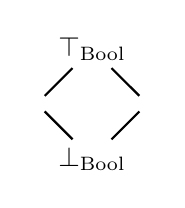
\begin{tikzpicture}
    \node (top) at (0,0) {$\top_{\mbox{\scriptsize Bool}}$};
    \node (midleft) at (-0.7,-0.7) {$\atrue$};
    \node (midright) at (0.7,-0.7) {$\afalse$};
    \node (down) at (0,-1.4) {$\bot_{\mbox{\scriptsize Bool}}$};
    \draw [black, thick, shorten <= -1pt, shorten >=-1pt] (top) -- (midleft);
    \draw [black, thick, shorten <= -1pt, shorten >=-1pt] (top) -- (midright);
    \draw [black, thick, shorten <= -1pt, shorten >=-1pt] (midleft) -- (down);
    \draw [black, thick, shorten <= -1pt, shorten >=-1pt] (midright) -- (down);
  \end{tikzpicture}
\end{matrix}
\quad
\abs{Absent} =
\begin{matrix}
  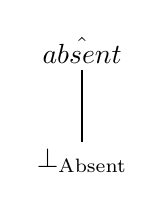
\begin{tikzpicture}
    \node (top) at (0,0) {$\hat{\SF{absent}}$};
    \node (down) at (0,-1.4) {$\bot_{\mbox{\scriptsize Absent}}$};
    \draw [black, thick, shorten <= -1pt, shorten >=-1pt] (top) -- (down);
  \end{tikzpicture}
\end{matrix}
\]
\[
\abs{Number} = 
\begin{matrix} 
  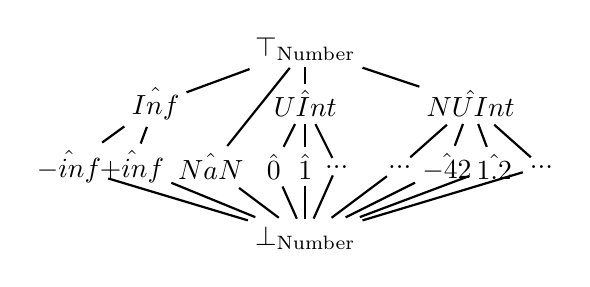
\begin{tikzpicture}
    % First, locate each of the nodes and name them
    \node (top) at (0,0) {$\top_{\mbox{\scriptsize Number}}$};
    \node (upperleft) at (-1.9,-0.7) {$\hat{\SF{Inf}}$};
    \node (uppercenter) at (0,-0.7) {$\hat{\SF{UInt}}$};
    \node (upperright) at (2.1,-0.7) {$\hat{\SF{NUInt}}$};
    \node (lower1) at (-3.0,-1.5) {$\hat{\SF{-inf}}$};
    \node (lower2) at (-2.2,-1.5) {$\hat{\SF{+inf}}$};
    \node (lower3) at (-1.2,-1.5) {$\hat{\SF{NaN}}$};
    \node (lower4) at (-0.4,-1.5) {$\hat{0}$};
    \node (lower5) at (0,-1.5) {$\hat{1}$};
    \node (lower6) at (0.4,-1.5) {...};
    \node (lower7) at (1.2,-1.5) {...};
    \node (lower8) at (1.8,-1.5) {$\hat{-42}$};
    \node (lower9) at (2.4,-1.5) {$\hat{1.2}$};
    \node (lower10) at (3,-1.5) {...};
    \node (down) at (0,-2.4) {$\bot_{\mbox{\scriptsize Number}}$};
    % Now draw the lines0
    \draw [black, thick, shorten <= -1pt, shorten >=-1pt] (top) -- (upperleft);
    \draw [black, thick, shorten <= -1pt, shorten >=-1pt] (top) -- (uppercenter);
    \draw [black, thick, shorten <= -1pt, shorten >=-1pt] (top) -- (upperright);
    \draw [black, thick, shorten <= -1pt, shorten >=-1pt] (top) -- (lower3);
    \draw [black, thick, shorten <= -1pt, shorten >=-1pt] (upperleft) -- (lower1);
    \draw [black, thick, shorten <= -1pt, shorten >=-1pt] (upperleft) -- (lower2);
    \draw [black, thick, shorten <= -1pt, shorten >=-1pt] (uppercenter) -- (lower4);
    \draw [black, thick, shorten <= -1pt, shorten >=-1pt] (uppercenter) -- (lower5);
    \draw [black, thick, shorten <= -1pt, shorten >=-1pt] (uppercenter) -- (lower6);
    \draw [black, thick, shorten <= -1pt, shorten >=-1pt] (upperright) -- (lower7);
    \draw [black, thick, shorten <= -1pt, shorten >=-1pt] (upperright) -- (lower8);
    \draw [black, thick, shorten <= -1pt, shorten >=-1pt] (upperright) -- (lower9);
    \draw [black, thick, shorten <= -1pt, shorten >=-1pt] (upperright) -- (lower10);
    \draw [black, thick, shorten <= -1pt, shorten >=-1pt] (lower1) -- (down);
    \draw [black, thick, shorten <= -1pt, shorten >=-1pt] (lower2) -- (down);
    \draw [black, thick, shorten <= -1pt, shorten >=-1pt] (lower3) -- (down);
    \draw [black, thick, shorten <= -1pt, shorten >=-1pt] (lower4) -- (down);
    \draw [black, thick, shorten <= -1pt, shorten >=-1pt] (lower5) -- (down);
    \draw [black, thick, shorten <= -1pt, shorten >=-1pt] (lower6) -- (down);
    \draw [black, thick, shorten <= -1pt, shorten >=-1pt] (lower7) -- (down);
    \draw [black, thick, shorten <= -1pt, shorten >=-1pt] (lower8) -- (down);
    \draw [black, thick, shorten <= -1pt, shorten >=-1pt] (lower9) -- (down);
    \draw [black, thick, shorten <= -1pt, shorten >=-1pt] (lower10) -- (down);
  \end{tikzpicture}
\end{matrix}
\]
\[
\abs{String} = 
	\begin{matrix} 
		\begin{tikzpicture}
	    % First, locate each of the nodes and name them
	    \node (top) at (0,0) {$\top_{\mbox{\scriptsize String}}$};
	    \node (upperleft) at (-1,-0.7) {$\hat{\SF{NumStr}}$};
	    \node (upperright) at (1,-0.7) {$\hat{\SF{OtherStr}}$};
	    \node (lower1) at (-2,-1.5) {$\hat{``\SF{NaN}"}$};
	    \node (lower2) at (-1.2,-1.5) {$\hat{``1.1"}$};
	    \node (lower3) at (-0.4,-1.5) {...};
	    \node (lower4) at (0.4,-1.5) {$\hat{``\mbox{foo}"}$};
	    \node (lower5) at (1.5,-1.5) {$\hat{``\mbox{bar}"}$};
	   	\node (lower6) at (2.2,-1.5) {...};
	    \node (down) at (0,-2.4) {$\bot_{\mbox{\scriptsize String}}$};
	    % Now draw the lines0
	  	\draw [black, thick, shorten <= -1pt, shorten >=-1pt] (top) -- (upperleft);
	  	\draw [black, thick, shorten <= -1pt, shorten >=-1pt] (top) -- (upperright);
	  	\draw [black, thick, shorten <= -1pt, shorten >=-1pt] (midleft) -- (lower1);
	  	\draw [black, thick, shorten <= -1pt, shorten >=-1pt] (midleft) -- (lower2);
	  	\draw [black, thick, shorten <= -1pt, shorten >=-1pt] (midleft) -- (lower3);
	  	\draw [black, thick, shorten <= -1pt, shorten >=-1pt] (midright) -- (lower4);
	  	\draw [black, thick, shorten <= -1pt, shorten >=-1pt] (midright) -- (lower5);
	  	\draw [black, thick, shorten <= -1pt, shorten >=-1pt] (midright) -- (lower6);
	  	\draw [black, thick, shorten <= -1pt, shorten >=-1pt] (lower1) -- (down);
	  	\draw [black, thick, shorten <= -1pt, shorten >=-1pt] (lower2) -- (down);
	  	\draw [black, thick, shorten <= -1pt, shorten >=-1pt] (lower3) -- (down);
	  	\draw [black, thick, shorten <= -1pt, shorten >=-1pt] (lower4) -- (down);
	  	\draw [black, thick, shorten <= -1pt, shorten >=-1pt] (lower5) -- (down);
	  	\draw [black, thick, shorten <= -1pt, shorten >=-1pt] (lower6) -- (down);
		\end{tikzpicture}
	\end{matrix}
\]

% % States                         
% \[
% \powerset{\SF{State}} \galois{\alpha_{state}}{\gamma_{state}} \abs{State}
% \]
% \[
% \begin{array}{lcl}
% \alpha_{state}(S) & = & (\hat{H})\\
% &&  \wherec{
%     \hat{H} = \alpha_{Heap}\left(\set{H \mid (H,A)\in S}\right) \\
% %    \hat{AS} = \bigcup\set{\alpha_{Env}(A) \mid (H,A)\in S} \\
%   } \\
% \end{array}
% \]

% % Heap
% \[
% \powerset{\SF{Heap}} \galois{\alpha_{heap}}{\gamma_{heap}} \aHeap
% \]
% \[
% \begin{array}{lcl}
% \alpha_{heap}(HS) & = & 
% \lambda \hat{l}.\alpha_{Obj}(\{o~\mid~ \hat{l}=\alpha_{Loc}(l) \land l\mapsto o\in HS \})
% \end{array}
% \]

% % Env
% \[
% \SF{Env} \galois{\alpha_{env}}{\gamma_{env}} \abs{Env}
% \]

% % Obj
% \[
% \powerset{\SF{Obj}} \galois{\alpha_{Obj}}{\gamma_{obj}} \aObj
% \]

% % PropValue
% \[
% \powerset{\SF{PropValue}} \galois{\alpha_{PropValue}}{\gamma_{PropValue}} \abs{PropValue}
% \]

% % ObjectValue
% \[
% \powerset{\SF{ObjectValue}} \galois{\alpha_{ObjectValue}}{\gamma_{ObjectValue}} \abs{ObjectValue}
% \]

% % Value
% \[
% \powerset{\Value} \galois{\alpha_{Value}}{\gamma_{Value}} \aValue
% \]

% % PValue
% \[
% \powerset{\SF{PValue}} \galois{\alpha_{PValue}}{\gamma_{PValue}} \abs{PValue}
% \]
\newpage
\section{Domain Operators}
\[
\begin{array}{ll}
\textit{Heap Order} & : \aHeap \times \aHeap \rightarrow \SF{Boolean} \\
& \hat{H}_1 \sqsubseteq \hat{H}_2 \defi dom(\hat{H}_1) \subseteq dom(\hat{H}_2) 
	\land \forall \hat{l} \in dom(\hat{H}_1): \hat{H}_1(\hat{l}) \sqsubseteq \hat{H}_2(\hat{l})\\
\\

\textit{Heap Join} & : \aHeap \times \aHeap \rightarrow \aHeap \\
& \hat{H}_1 \sqcup \hat{H}_2  \defi \forall \hat{l} \in dom(\hat{H}_1) \cup dom(\hat{H}_2): 
  \left\{
    \begin{array}{ll}
      \left[\hat{l} \mapsto \hat{H}_1(\hat{l}) \sqcup \hat{H}_2(\hat{l})\right] & \ifc{\hat{l} \in dom(\hat{H}_1)\land \hat{l} \in dom(\hat{H}_2)}\\
      \left[\hat{l} \mapsto \hat{H}_2(\hat{l}) \right] & \ifc{\hat{l} \not\in dom(\hat{H}_1)\land \hat{l} \in dom(\hat{H}_2)}\\
      \left[\hat{l} \mapsto \hat{H}_1(\hat{l}) \right] & \ifc{\hat{l} \in dom(\hat{H}_1)\land \hat{l} \not\in dom(\hat{H}_2)}\\
    \end{array}
  \right.\\
\\

\textit{Heap Domain In} & : \aHeap \times \aLoc \rightarrow \SF{Boolean} \\
& \hat{l} \in dom(\hat{H}) \defi
 \left\{
   \begin{array}{ll}
     \SF{true}
     & \ifc{\hat{l} \in \{ \hat{l}'\ |\ (\hat{l}', \hat{o}) \in \hat{H}\}} \\
     \SF{false}
     & \owc \\
   \end{array}
 \right.\\
\\

& {\inblue \textit{Although $\bot_{Obj}$ is returned for non-existent locations, heap is still partial function.}} \\
\textit{Heap Lookup} & : \aHeap \times \aLoc \rightarrow \aObj \\
& \hat{H}(\hat{l}) \defi
 \left\{
   \begin{array}{ll}
      \hat{o} & \ifc{(\hat{l}, \hat{o}) \in \hat{H}} \\
      \bot_{Obj} & \owc
   \end{array}
 \right.\\
\\

\textit{Heap Update} & : \aHeap \times \aLoc \times \aObj \rightarrow \aHeap \\
& \hat{H}[\hat{l} \mapsto \hat{o}] \defi
 \left\{
   \begin{array}{ll}
      \{( \hat{l}, \hat{o})\} \cup (\hat{H}-\hat{l})
      & \ifc{\hat{l} = \hat{l}_R \land \hat{o} \neq \bot_{Obj}} \\
      \bot_{Heap} 
      & \ifc{\hat{l} = \hat{l}_R \land \hat{o} = \bot_{Obj}} \\
      \{( \hat{l}, \hat{H}(\hat{l}) \sqcup \hat{o})\} \cup (\hat{H}-\hat{l})
      & \ifc{\hat{l} = \hat{l}_O \land \hat{H}(\hat{l}) \sqcup \hat{o} \neq \bot_{Obj}} \\
      \bot_{Heap} 
      & \ifc{\hat{l} = \hat{l}_O \land \hat{H}(\hat{l}) \sqcup \hat{o} = \bot_{Obj}} \\
   \end{array}
 \right.\\
\\\\


\textit{Context Order} & : \abs{Context} \times \abs{Context} \rightarrow \SF{Boolean} \\
& \hat{C}_1 \sqsubseteq \hat{C}_2 \defi 
  \begin{array}[t]{l}
    \hat{C}_1.3 \subseteq \hat{C}_2.3 ~~ \land \\
    \hat{C}_1.4 \supseteq \hat{C}_2.4 \quad\quad\comment{{\inblue order is opposite for must old set}}
  \end{array} \\
\\

\textit{Context Join} & : \abs{Context} \times \abs{Context} \rightarrow \abs{Context} \\
& \hat{C}_1 \sqcup \hat{C}_2 \defi 
  \langle
    {\inred \{ \}, \{ \}},\ 
    \hat{C}_1.3 \cup \hat{C}_2.3,\ 
    \hat{C}_1.4 \cap \hat{C}_2.4
  \rangle \\
\\\\


\textit{Obj Order} & : \aObj \times \aObj \rightarrow \SF{Boolean} \\
& \hat{o}_1 \sqsubseteq \hat{o}_2 \defi \forall x \in dom(\hat{o}_1) \cup dom(\hat{o}_2): \hat{o}_1(x) \sqsubseteq \hat{o}_2(x)\\
\\
\textit{Obj Join} & : \aObj \times \aObj \rightarrow \aObj \\
& \hat{o}_1 \sqcup \hat{o}_2  \defi \forall x \in dom(\hat{o}_1) \cup dom(\hat{o}_2): \left[x \mapsto \hat{o}_1(x) \sqcup \hat{o}_2(x)\right]\\
\\

\textit{Obj Domain In} & : \aObj \times \abs{String} \rightarrow \abs{Bool} \\
& \hat{s} \dot{\in} dom(\hat{o}) \defi
     \left\{
       \begin{array}{ll}
         x \dot{\in} dom(\hat{o})
         & \ifc{\hat{o} \neq \bot_{Obj} \land \hat{s} = \hat{\SF{NumStrSingle}}(x) }\\
         x \dot{\in} dom(\hat{o})
         & \ifc{\hat{o} \neq \bot_{Obj} \land \hat{s} = \hat{\SF{OtherStrSingle}}(x) }\\
         \hat{b}_1
         & \ifc{\hat{o} \neq \bot_{Obj} \land \hat{s} = \hat{\SF{NumStr}} }\\
         \hat{b}_2
         & \ifc{\hat{o} \neq \bot_{Obj} \land \hat{s} = \hat{\SF{OtherStr}} }\\
         \hat{b}_3
         & \ifc{\hat{o} \neq \bot_{Obj} \land \hat{s} = \top_{String} }\\
         \bot_{Bool} 
         & \ifc{\hat{o} = \bot_{Obj} \lor \hat{s} = \bot_{String} }\\
       \end{array}
     \right.\\
 & \quad\wherec{
   \hat{b}_1 = 
     \left\{
       \begin{array}{ll}
         \top_{Bool} & \ifc{\hat{o}(\emph{@default\_number}).1.1.1 \not\sqsubseteq \bot_{Value}}\\
         \top_{Bool} & \ifc{\hat{o}(\emph{@default\_number}).1.1.1 \sqsubseteq \bot_{Value}}\\
                     & \quad \land\ \exists x \in dom(\hat{o}):x \in \SF{String} \land \hat{``x"} \sqsubseteq \hat{\SF{NumStr}}\\
         \afalse & \owc\\
       \end{array}
     \right.\\
   \hat{b}_2 = 
     \left\{
       \begin{array}{ll}
         \top_{Bool} & \ifc{\hat{o}(\emph{@default\_other}).1.1.1 \not\sqsubseteq \bot_{Value}}\\
         \top_{Bool} & \ifc{\hat{o}(\emph{@default\_other}).1.1.1 \sqsubseteq \bot_{Value}}\\
                     & \quad \land\ \exists x \in dom(\hat{o}):x \in \SF{String} \land \hat{``x"} \sqsubseteq \hat{\SF{OtherStr}}\\
         \afalse & \owc\\
       \end{array}
     \right.\\
   \hat{b}_3 = 
     \left\{
       \begin{array}{ll}
         \top_{Bool} 
         & \ifc{\hat{o}(\emph{@default\_number}).1.1.1 \not\sqsubseteq \bot_{Value}\vee \hat{o}(\emph{@default\_other}).1.1.1 \not\sqsubseteq \bot_{Value}}\\
         \top_{Bool} 
         & \ifc{\hat{o}(\emph{@default\_number}).1.1.1 \sqsubseteq \bot_{Value}\land \hat{o}(\emph{@default\_other}).1.1.1 \sqsubseteq \bot_{Value}}\\
         & \quad \land\ \exists x \in dom(\hat{o}):x \in \SF{String}\\
         \afalse & \owc\\
       \end{array}
     \right.\\ 
  }\\
\end{array}
\]

\[
\begin{array}{ll}
\textit{Obj Domain In} & : \aObj \times \SF{Prop} \rightarrow \abs{Bool} \\
& x \dot{\in} dom(\hat{o}) \defi
  \left\{
    \begin{array}{ll}
      \hat{b} & \ifc{\hat{o} \neq \bot_{Obj}} \\
      \bot_{Bool} & \ifc{\hat{o} = \bot_{Obj}}
    \end{array}
  \right. \\
& \quad\wherec{
  \hat{b} = 
    \left\{
      \begin{array}{ll}
        \atrue
        &\ifc{\hat{o}(x)\not\sqsubseteq\bot \land \hat{\SF{absent}}\not\sqsubseteq\hat{o}(x).2}\\
        \top_{Bool}
        &\ifc{\hat{o}(x)\not\sqsubseteq\bot \land \hat{\SF{absent}}\sqsubseteq\hat{o}(x).2}\\
        \top_{Bool}
        &\ifc{\hat{o}(x)\sqsubseteq\bot \land x\in \SF{String} \land \alpha(x) \sqsubseteq \hat{\SF{NumStr}}}\\
        & \quad\land \hat{o}(\emph{@default\_number}).1.1.1 \not\sqsubseteq \bot_{Value} \\
        \top_{Bool}
        &\ifc{\hat{o}(x)\sqsubseteq\bot \land x\in \SF{String} \land \alpha(x) \sqsubseteq \hat{\SF{OtherStr}}}\\
        & \quad\land \hat{o}(\emph{@default\_other}).1.1.1 \not\sqsubseteq \bot_{Value} \\
        \afalse
        &\ifc{\hat{o}(x)\sqsubseteq\bot \land x\in \SF{String} \land \alpha(x) \sqsubseteq \hat{\SF{NumStr}}}\\
        & \quad\land \hat{o}(\emph{@default\_number}).1.1.1 \sqsubseteq \bot_{Value} \\
        \afalse
        &\ifc{\hat{o}(x)\sqsubseteq\bot \land x\in \SF{String} \land \alpha(x) \sqsubseteq \hat{\SF{OtherStr}}}\\
        & \quad\land \hat{o}(\emph{@default\_other}).1.1.1 \sqsubseteq \bot_{Value} \\
        \afalse
        &\ifc{\hat{o}(x)\sqsubseteq\bot \land x\not\in \SF{String}}\\
        \afalse&\owc\\
      \end{array}
    \right.
}
\\\\

\textit{Obj Lookup} & : \aObj \times \abs{String} \rightarrow \abs{PropValue} \times \abs{Absent}\\
& \hat{o}(\hat{s}) \defi
     \left\{
       \begin{array}{ll}
         \hat{o}(x)
         & \ifc{\hat{s} = \hat{\SF{NumStrSingle}}(x) }\\
         \hat{o}(x)
         & \ifc{\hat{s} = \hat{\SF{OtherStrSingle}}(x) }\\
         \langle (\bigsqcup_{x \in P_1} \hat{o}(x)).1 \sqcup \hat{o}(\emph{@default\_number}).1, \top_{Absent}\rangle
         & \ifc{\hat{s} = \hat{\SF{NumStr}} }\\
         \langle (\bigsqcup_{x \in P_2} \hat{o}(x)).1 \sqcup \hat{o}(\emph{@default\_other}).1, \top_{Absent}\rangle
         & \ifc{\hat{s} = \hat{\SF{OtherStr}} }\\
         \left\langle 
           \begin{matrix}
             (\bigsqcup_{x \in P_3} \hat{o}(x)).1 \sqcup \hat{o}(\emph{@default\_number}).1 \\ 
             \sqcup \hat{o}(\emph{@default\_other}).1
           \end{matrix},
         \top_{Absent}\right\rangle
         & \ifc{\hat{s} = \top_{String} }\\
         \bot_{PropValue \times Absent} 
         &\ifc{\hat{s} = \bot_{String} }\\
       \end{array}
     \right.\\
 & \quad\wherec{
   P_1 = \{ x\ |\ x \in dom(\hat{o}) \land x \in \SF{String} \land \hat{``x"} \sqsubseteq \hat{\SF{NumStr}}\}\\
   P_2 = \{ x\ |\ x \in dom(\hat{o}) \land x \in \SF{String} \land \hat{``x"} \sqsubseteq \hat{\SF{OtherStr}}\}\\
   P_3 = \{ x\ |\ x \in dom(\hat{o}) \land x \in \SF{String}\}\\
  }\\
\\\\
\textit{Obj Lookup} & : \aObj \times \SF{Prop} \rightarrow \abs{PropValue} \times \abs{Absent} \\
& \hat{o}(x) \defi 
  \left\{
    \begin{array}{ll}
      \langle\hat{propv}, \hat{abs}\rangle
      & \ifc{\begin{array}{l}x \rightarrow \langle\hat{propv}, \hat{abs}\rangle \in \hat{o}\end{array}} \\
      \langle\bot_{PropValue}, \bot_{Absent}\rangle
      & \ifc{\begin{array}{l}x \rightarrow \langle\hat{propv}, \hat{abs}\rangle \not\in \hat{o} \land x \not\in \SF{String} \end{array}}\\
      \langle\hat{propv}_2, \hat{abs}_2\rangle
      & \ifc{ \begin{array}{l}
          x \rightarrow \langle\hat{propv}_1, \hat{abs}_1\rangle \not\in \hat{o} \land x \in \SF{String}\\
          \land \alpha(x) \sqsubseteq \hat{\SF{NumStr}}
          \land \emph{@default\_number} \rightarrow
          \langle\hat{propv}_2, \hat{abs}_2\rangle \in \hat{o}\end{array}}\\
      \langle\hat{propv}_3, \hat{abs}_3\rangle
      & \ifc{ \begin{array}{l}
          x \rightarrow \langle\hat{propv}_1, \hat{abs}_1\rangle \not\in \hat{o} \land x \in \SF{String}\\
          \land \alpha(x) \sqsubseteq \hat{\SF{OtherStr}}
          \land \emph{@default\_other} \rightarrow
          \langle\hat{propv}_3, \hat{abs}_3\rangle \in \hat{o}\end{array}}\\
    \end{array}
  \right.\\
\\

\end{array}
\]

\[
\begin{array}{ll}
\textit{Obj Update} & : \aObj \times \abs{String} \times \abs{PropValue} \rightarrow \aObj \\
& \hat{o}[\hat{s} \mapsto \hat{propv}] \defi 
 \left\{
       \begin{array}{ll}
         \hat{o}[x \mapsto \hat{propv}]
         & \ifc{\hat{o} \neq \bot_{Obj} \land \hat{s} = \hat{\SF{NumStrSingle}}(x) }\\
         \hat{o}[x \mapsto \hat{propv}]
         & \ifc{\hat{o} \neq \bot_{Obj} \land \hat{s} = \hat{\SF{OtherStrSingle}}(x) }\\
         \hat{o}
         \left[
           \begin{array}{l}
           \forall x \in P_1 : x \mapsto \hat{o}(x) \sqcup \hat{propv},\\
           \emph{@default\_number} \mapsto \hat{o}(\emph{@default\_number}) \sqcup \hat{propv}\\
           \end{array}
         \right]
         & \ifc{\hat{o} \neq \bot_{Obj} \land \hat{s} = \hat{\SF{NumStr}} }\\
         \hat{o}
         \left[
           \begin{array}{l}
           \forall x \in P_2 : x \mapsto \hat{o}(x) \sqcup \hat{propv},\\
           \emph{@default\_other} \mapsto \hat{o}(\emph{@default\_other}) \sqcup \hat{propv}\\
           \end{array}
         \right]
         & \ifc{\hat{o} \neq \bot_{Obj} \land \hat{s} = \hat{\SF{OtherStr}} }\\
         \hat{o}
         \left[
           \begin{array}{l}
           \forall x \in P_3 : x \mapsto \hat{o}(x) \sqcup \hat{propv},\\
           \emph{@default\_number} \mapsto \hat{o}(\emph{@default\_number}) \sqcup \hat{propv},\\
           \emph{@default\_other} \mapsto \hat{o}(\emph{@default\_other}) \sqcup \hat{propv}\\
           \end{array}
         \right]
         & \ifc{\hat{o} \neq \bot_{Obj} \land \hat{s} = \top_{String} }\\
         \bot_{Obj}
         & \ifc{\hat{o} = \bot_{Obj} \lor \hat{s} = \bot_{String} }\\
       \end{array}
     \right.\\
& \quad\wherec{
   P_1 = \{ x\ |\ x \in dom(\hat{o}) \land x \in \SF{String} \land \hat{``x"} \sqsubseteq \hat{\SF{NumStr}}\}\\
   P_2 = \{ x\ |\ x \in dom(\hat{o}) \land x \in \SF{String} \land \hat{``x"} \sqsubseteq \hat{\SF{OtherStr}}\}\\
   P_3 = \{ x\ |\ x \in dom(\hat{o}) \land x \in \SF{String}\}\\
  }\\
\\\\
\textit{Obj Update} & : \aObj \times \SF{Prop} \times \abs{PropValue} \rightarrow \aObj \\
& \hat{o}[x \mapsto \hat{propv}] \defi 
  \left\{
    \begin{array}{ll}
      \{( x, \langle \hat{propv}, \bot_{Absent} \rangle)\} \cup (\hat{o}\setminus\{(x,\langle \hat{propv}', \hat{abs}' \rangle)\}) 
        & \ifc{\hat{o} \neq \bot_{Obj}} \\
      \bot_{Obj} & \ifc{\hat{o} = \bot_{Obj}} \\
    \end{array}
  \right.
\\\\
\textit{Obj Update} & : \aObj \times \SF{Prop} \times \abs{PropValue} \times \abs{Absent} \rightarrow \aObj \\
& \hat{o}[x \mapsto \langle \hat{propv}, \hat{abs} \rangle] \defi 
  \left\{
    \begin{array}{ll}
      \{( x, \langle \hat{propv}, \hat{abs} \rangle)\} \cup (\hat{o}\setminus\{(x,\langle \hat{propv}', \hat{abs}' \rangle)\}) 
        & \ifc{\hat{o} \neq \bot_{Obj}} \\
      \bot_{Obj} & \ifc{\hat{o} = \bot_{Obj}} \\
    \end{array}
  \right.
%\textit{Obj Update} & : \aObj \times \SF{Prop} \times \abs{PropValue} \times \abs{Absent} \rightarrow \aObj \\
%& \hat{o}[x \mapsto \langle \hat{propv}, \hat{abs} \rangle] \defi \{( x, \langle \hat{propv}, \hat{abs} \rangle)\} \cup (\hat{o}\setminus\{(x,\langle \hat{propv}', \hat{abs}' \rangle)\})\\
\\\\
\textit{Obj Remove} & : \aObj \times \abs{String} \rightarrow \aObj \\
& \hat{o}- \hat{s} \defi 
 \left\{
       \begin{array}{ll}
         \hat{o} - x
         & \ifc{\hat{o} \neq \bot_{Obj} \land \hat{s} = \hat{\SF{NumStrSingle}}(x) }\\
         \hat{o} - x
         & \ifc{\hat{o} \neq \bot_{Obj} \land \hat{s} = \hat{\SF{OtherStrSingle}}(x) }\\
          \hat{o} \sqcup \bigsqcup_{x \in P_1}\ \{ (y,\langle \hat{propv}, \hat{abs}\rangle)\ |\ (y,\langle \hat{propv}, \hat{abs}\rangle) \in \hat{o} \land y \neq x \}
         & \ifc{\hat{o} \neq \bot_{Obj} \land \hat{s} = \hat{\SF{NumStr}} }\\
          \hat{o} \sqcup \bigsqcup_{x \in P_2}\ \{ (y,\langle \hat{propv}, \hat{abs}\rangle)\ |\ (y,\langle \hat{propv}, \hat{abs}\rangle) \in \hat{o} \land y \neq x \}
         & \ifc{\hat{o} \neq \bot_{Obj} \land \hat{s} = \hat{\SF{OtherStr}} }\\
          \hat{o} \sqcup \bigsqcup_{x \in P_3}\ \{ (y,\langle \hat{propv}, \hat{abs}\rangle)\ |\ (y,\langle \hat{propv}, \hat{abs}\rangle) \in \hat{o} \land y \neq x \}
         & \ifc{\hat{o} \neq \bot_{Obj} \land \hat{s} = \top_{String} }\\
         \bot_{Obj}
         & \ifc{\hat{o} = \bot_{Obj} \lor \hat{s} = \bot_{String} }\\
       \end{array}
     \right.\\
& \quad\wherec{
   P_1 = \{ x\ |\ x \in dom(\hat{o}) \land x \in \SF{String} \land \atrue \sqsubseteq \hat{o}(x).1.1.4 \land \hat{``x"} \sqsubseteq \hat{\SF{NumStr}} \}\\
   P_2 = \{ x\ |\ x \in dom(\hat{o}) \land x \in \SF{String} \land \atrue \sqsubseteq \hat{o}(x).1.1.4 \land \hat{``x"} \sqsubseteq \hat{\SF{OtherStr}}\}\\
   P_3 = \{ x\ |\ x \in dom(\hat{o}) \land x \in \SF{String} \land \atrue \sqsubseteq \hat{o}(x).1.1.4\}\\
  }\\
\\\\
\textit{Obj Remove} & : \aObj \times \SF{Prop} \rightarrow \aObj \\
& \hat{o}- x \defi 
  \left\{
  \begin{array}{ll}
    \{ (y,\langle \hat{propv}, \hat{abs}\rangle)\ |\ (y,\langle \hat{propv}, \hat{abs}\rangle) \in \hat{o} \land y \neq x \} 
    & \ifc{\hat{o} \neq \bot_{Obj}} \\
    \bot_{Obj} & \ifc{\hat{o} = \bot_{Obj}} \\
  \end{array}
  \right.\\
\\\\
%\rel^t &: \abs{IROP} \rightarrow \abs{IROP}\\
\rel^t &: \SF{IRRelOP} \rightarrow \SF{IRRelOP}\\
& \rel^ t = \left\{
  \begin{array}{ll}
    < & \ifc{ \rel ~=~ >}\\
    <= & \ifc{ \rel ~=~ >=}\\
    > & \ifc{ \rel ~=~ <}\\
    >= & \ifc{ \rel ~=~ <=}\\
    \rel & \owc \\
  \end{array}
\right.\\
\\\\
\end{array}
\]

\newpage
\section{Helper Functions}
{\inblue\tt .../jsaf/analysis/typing/Helper.scala}

%%% CanPut %%%
\[
\begin{array}{ll}
\ahf{CanPut} & : \aHeap \times \aLoc \times \abs{String} \rightarrow \abs{Bool}\\
&
\begin{array}{ll}
  \ahf{CanPut}(\hat{H},\hat{l},\hat{s}) = \ahf{CanPutHelp}(\hat{H},\hat{l},\hat{s},\hat{l}) & \\
\end{array}
\\\\

%& {\inblue \textit{For all case of }\hat{s}_n\textit{ if the condition is false, the value of }\hat{s}_n\textit{ is }\bot_{String}.} \\
& {\inblue \textit{Cycle in prototype chain is detected at implementation level.}} \\
\ahf{CanPutHelp} &  : \aHeap \times \aLoc \times \abs{String} \times \aLoc \rightarrow \abs{Bool}\\
&  \ahf{CanPutHelp}(\hat{H},\hat{l}_1,\hat{s},\hat{l}_2)  = \hat{b}_1\sqcup\hat{b}_2\\
&  \quad\wherec{
    \hat{b}_1 =
    \left\{
      \begin{array}{ll}
        \hat{H}(\hat{l}_1)(\hat{s}).1.1.2
        ~~{\inblue \textit{// writable attribute}}
        & \ifc{\atrue\sqsubseteq(\hat{s} \dot{\in} dom(\hat{H}(\hat{l})))}\\
        \bot_{Bool} & \owc\\
      \end{array}
    \right.\\
    \hat{L}_{proto}=\hat{H}(\hat{l}_1)(\varprop{proto}).1.1.1.2
~~{\inblue \textit{// $\powerset{\aLoc}$ type}}\\
    \hat{b}_2 =
    \left\{
      \begin{array}{ll}
        \hat{b}_3 \sqcup \bigsqcup_{\hat{l}_{proto}\in\hat{L}_{proto}}\ahf{CanPutHelp}(\hat{H},\hat{l}_{proto},\hat{s},\hat{l}_2)& \ifc{\afalse\sqsubseteq(\hat{s} \dot{\in} dom(\hat{H}(\hat{l})))}\\
        \bot_{Bool} & \owc\\
      \end{array}
    \right.\\
    \hat{b}_3 =
    \left\{
      \begin{array}{ll}
        \hat{H}(\hat{l}_2)(\varprop{extensible}).1.2.1.3& \ifc{\hat{H}(\hat{l}_1)(\varprop{proto}).1.1.1.1.2 \not\sqsubseteq \bot_{Null}}\\
        \bot_{Bool} & \owc\\
      \end{array}
    \right.\\
    }\\
\\

\ahf{CanPutVar} & : \aHeap \times \SF{Prop} \rightarrow \abs{Bool}\\
&
\begin{array}{ll}
\ahf{CanPutVar}(\hat{H},x)
  =  \hat{b}_1\sqcup\hat{b}_2\\
  \quad\wherec{
    \hat{b}_1 =
      \left\{
        \begin{array}{ll}
          \hat{H}(\avarloc{Global}_R)(x).1.1.2 & \ifc{\atrue\sqsubseteq(x \dot{\in} dom(\hat{H}(\avarloc{Global})))} \\
          \bot_{Bool} & \owc \\
        \end{array}
      \right.\\
    \hat{b}_2 = 
      \left\{
        \begin{array}{ll}
          \ahf{CanPut}(\hat{H},\avarloc{Global}_R,\hat{x}) & \ifc{\afalse\sqsubseteq(x \dot{\in} dom(\hat{H}(\avarloc{Global})))} \\
          \bot_{Bool} & \owc \\
        \end{array}
      \right.\\
  }
\end{array}\\
\\

\\

%%% CreateMutableBinding %%%


& {\inblue \textit{Temporaries and pure local variables are always mutable in non-strict mode.}} \\
& {\inblue \textit{In strict-mode, ``arguments" is immutable AND pure local, which invalidates current approach.}} \\
\ahf{CreateMutableBinding} & : \aHeap \times \SF{Prop} \times \SF{Value} \rightarrow \aHeap \\
& \ahf{CreateMutableBinding}(\hat{H}, x, \hat{v}) = \hat{H}_1 \quad\ifc{\chf{getVarKind}_P(x) = \SF{PureLocalVar}} \\
& \quad\wherec{\hat{H}_1 = \hat{H}[\avarloc{PureLocal}_R \mapsto \hat{H}(\avarloc{PureLocal}_R)
    [x \mapsto \langle \hat{v},\bot_{Bool},\bot_{Bool},\afalse \rangle]]} \\
& \ahf{CreateMutableBinding}(\hat{H}, x, \hat{v}) = \hat{H}_1 \quad\ifc{\chf{getVarKind}_P(x) = \SF{CapturedVar}} \\
& \quad\wherec{\hat{H}_1 = \bigsqcup_{\hat{l}\in\hat{H}(\avarloc{PureLocal}_R)(\varprop{env}).1.2.2} \hat{H}[\hat{l} \mapsto \hat{H}(\hat{l})
    [x \mapsto \langle \hat{v},\atrue,\bot_{Bool},\afalse \rangle]]} \\
& \ahf{CreateMutableBinding}(\hat{H}, x, \hat{v}) = \hat{H}_1 \quad\ifc{\chf{getVarKind}_P(x) = \SF{CapturedCatchVar}} \\
& \quad\wherec{\hat{H}_1 = \hat{H}[\avarloc{Collapsed}_O \mapsto \hat{H}(\avarloc{Collapsed}_O)
    [x \mapsto \langle \hat{v},\bot_{Bool},\bot_{Bool},\afalse \rangle]]} \\
& \ahf{CreateMutableBinding}(\hat{H}, x, \hat{v}) = \hat{H}_1 \quad\ifc{\chf{getVarKind}_P(x) = \SF{GlobalVar}} \\
& \quad\wherec{\hat{H}_1 = \hat{H}[\avarloc{Global}_R \mapsto \hat{H}(\avarloc{Global}_R)
    [x \mapsto \langle \hat{v},\atrue,\atrue,\afalse \rangle]]} \\
\\
\end{array}
\]
\\

%%% Delete %%%
\[
\begin{array}{ll}

& {\inblue \hat{H}(\hat{l})(\hat{s}).1.1.4\textit{ means the configurable attribute of the property.}} \\
\ahf{Delete} & : \aHeap \times \aLoc \times \abs{String} \rightarrow \aHeap
\times \abs{Bool}\\
& \ahf{Delete}(\hat{H},\hat{l},\hat{s})
  = (\hat{H}_1\sqcup\hat{H}_2,\hat{b}_1\sqcup\hat{b}_2)\\
&  \quad\wherec{
%    (\hat{H}_1,\hat{b}_1) = \left\{
%      \begin{array}{ll}
%        (\hat{H},\atrue)
%        & \ifc{\afalse\sqsubseteq\ahf{HasOwnProperty}(\hat{H},\hat{l},x)} \\
%        \bot_{Heap\times Bool} & \owc \\
%      \end{array}
%    \right.\\
    (\hat{H}_1,\hat{b}_1) = \left\{
      \begin{array}{ll}
        (\hat{H},\afalse)
        & \ifc{\atrue\sqsubseteq\ahf{HasOwnProperty}(\hat{H},\hat{l},\hat{s})
          \land\ \afalse\sqsubseteq\hat{H}(\hat{l})(\hat{s}).1.1.4}\\
        \bot_{Heap\times Bool} & \owc \\
      \end{array}
    \right.\\
%{\inblue \textit{If the value is deleted in update operation,}}\\
%{\inblue \textit{the absent attribute of the value will be 'absent' instead of removing the value}}\\
%{\inblue \textit{because of a weak update.}}\\
    (\hat{H}_2,\hat{b}_2) = \left\{
      \begin{array}{ll}
        (\hat{H}[\hat{l}\mapsto \hat{H}(\hat{l}) - \hat{s}],\atrue)
        & \ifc{
          \begin{array}{l}
            \left(
              \begin{array}{l}
              \atrue \sqsubseteq\ahf{HasOwnProperty}(\hat{H},\hat{l},\hat{s})\\
              \land \atrue\sqsubseteq\hat{H}(\hat{l})(\hat{s}).1.1.4)
              \end{array}
            \right)\\
            \vee (\afalse\sqsubseteq\ahf{HasOwnProperty}(\hat{H},\hat{l},\hat{s}))
          \end{array}}\\
        \bot_{Heap\times Bool} & \owc \\
      \end{array}
    \right.\\
  }\\
\\

\ahf {DeleteAll} &: \aHeap \times \aLoc \times \abs{String} \rightarrow \aHeap\\
& \ahf{DeleteAll} (\hat{H}, \hat{l}, \hat{s}) = \hat{H}_1\\
& \quad\wherec{
  \hat{H}_2 = \ahf{Delete}(\hat{H}, \hat{l}, \hat{s}).1\\
  \hat{H}_1 = \left\{
    \begin{array}{ll}
      \ahf{DeleteAll}(\hat{H}_2, \hat{l}_1, \hat{s}) & \ifc{\hat{H}(\hat{l})(@proto).1.1.1.1.2 \sqsubseteq \bot_{Null} \\ \land \hat{H}(\hat{l})(@proto).1.1.1.2 = \{ \hat{l}_1\}}\\
      \hat{H}_2 & \owc
    \end{array}
  \right.
}
\\

\\

%Exception


\ahf{RaiseException} & : \aHeap \times \abs{Context} \times \powerset{\abs{Exception}} \rightarrow \aHeap \times \abs{Context}\\
 & \ahf{RaiseException}(\hat{H},\hat{C}, \hat{es}) = (\hat{H}_1, \hat{C}_1) \\
 & \quad\wherec{
   \hat{v}_{old} = \hat{H}(\avarloc{PureLocal}_R)(\varprop{exception\_all}).1.2 \\
   \hat{v}_e = \langle \bot_{PValue},\ \bigsqcup_{\hat{exc}\in\hat{es}}\ahf{NewExceptionLoc}(\hat{exc}) \rangle \\
   \hat{H}_e = \hat{H}\left[\avarloc{PureLocal}_R\mapsto \hat{H}(\avarloc{PureLocal}_R)
     \left[\begin{array}{l}
         \varprop{exception}\mapsto \hat{v}_e, \\
         \varprop{exception\_all}\mapsto \hat{v}_e \sqcup \hat{v}_{old} 
     \end{array}\right]\right]\\
   (\hat{H}_1, \hat{C}_1) = \left\{
     \begin{array}{ll}
       (\hat{H}_e, \hat{C})&\quad\ifc{\hat{es} \neq \{\}}\\
       (\bot_{Heap}, \bot_{Context}) &\quad\owc
     \end{array}
   \right.\\
}\\
\\

\ahf{NewExceptionLoc} & : \abs{Exception} \rightarrow \abs{Loc} \\
 & \ahf{NewExceptionLoc}(\hat{H},\hat{exc}) =
 \left\{
   \begin{array}{ll}
     \avarloc{Err}_O & \ifc{\hat{exc} = \hat{\exc{Error}}} \\
     \avarloc{EvalErr}_O & \ifc{\hat{exc} = \hat{\exc{EvalError}}} \\
     \avarloc{RangeErr}_O & \ifc{\hat{exc} = \hat{\exc{RangeError}}} \\
     \avarloc{RefErr}_O & \ifc{\hat{exc} = \hat{\exc{ReferenceError}}} \\
     \avarloc{SyntaxErr}_O & \ifc{\hat{exc} = \hat{\exc{SyntaxError}}} \\
     \avarloc{TypeErr}_O & \ifc{\hat{exc} = \hat{\exc{TypeError}}} \\
     \avarloc{URIErr}_O & \ifc{\hat{exc} = \hat{\exc{URIError}}} \\
   \end{array}
 \right.\\
\\
\end{array}
\]
\\

%%% get %%%
\[
\begin{array}{ll}

\ahf{getRel} & : \SF{RelExpr} \rightarrow \aState \rightarrow \powerset{\SF{RelExpr}}\\
%& \ahf{getRel}(\hat{re}, \hat{S}) = \hat{re}_1 \sqcup \hat{re}_2 \sqcup \hat{re}_3\\
%& \quad\wherec{
%  (\hat{H}, \hat{C}) = \hat{S}\\
%  e_1 \rel e_2 = \hat{re}\\
%  b = \ahf{validity}(\aV \lbr e_2 \rbr (\hat{H}, \hat{C}).1) \land b_1\\
%  b_1 = \left\{
%    \begin{array}{ll}
%      \ahf{validity}(\aV \lbr e_3 \rbr (\hat{H}, \hat{C}).1) \land \ahf{validity}(\aV \lbr e_4 \rbr (\hat{H}, \hat{C}).1) & \ifc { e_3 \otimes e_4 = e_1}\\
%      \vfalse & \owc\\
%    \end{array}
%  \right.\\
%  \hat{re}_1 = \left\{
%    \begin{array}{ll}
%      \{\hat{re}\} &  \ifc{ e_1 \in \$\sf{Expression}}\\
%      \{\} & \owc
%    \end{array}
%   \right.\\
%  \hat{re}_2 = \left\{
%    \begin{array}{ll}
%      \ahf{getRel}(e_3 \rel ( e_2 - e_4 ), \hat{S} ) \sqcup \ahf{getRel}(e_4 \rel ( e_2 - e_3 ), \hat{S} ) &  \ifc{ e_3 + e_4 = e_1 \land b}\\
%      \ahf{getRel}(e_3 \rel ( e_2 + e_4 ), \hat{S} ) \sqcup \ahf{getRel}(e_4 \rel^t ( e_2 - e_3 ), \hat{S} ) &  \ifc{ e_3 - e_4 = e_1 \land b}\\
%      \{\} & \owc
%    \end{array}
%   \right.\\
%  \hat{re}_3 = \left\{
%    \begin{array}{ll}
%      \ahf{getRel}((e_3 * n ) \rel e_2, \hat{S} ) &  \ifc{ n * e_3 = e_1 \land b}\\
%      \ahf{getRel}(e_3 \rel ( e_2 / n), \hat{S} ) &  \ifc{ e_3 * n = e_1 \land b \land n > 0}\\
%      \ahf{getRel}(e_3 \rel ( e_2 * n), \hat{S} ) &  \ifc{ e_3 / n = e_1 \land b \land n > 0}\\
%      \ahf{getRel}(e_3 \rel^t ( e_2 / n), \hat{S} ) &  \ifc{ e_3 * n = e_1 \land b \land n < 0}\\
%      \ahf{getRel}(e_3 \rel^t ( e_2 * n), \hat{S} ) &  \ifc{ e_3 / n = e_1 \land b \land n < 0}\\
%      \{\} & \owc
%    \end{array}
%   \right.\\
%}\\
& \begin{array}{lll}
  \ahf{getRel}(pe \rel e, \hat{S}) &=& \{pe \rel e\}\\
  \ahf{getRel}((e_1 + e_2) \rel e_3, \, \hat{S})  &=& \ahf{getRel} (e_1 \rel (e_3 - e_2), \hat{S}) \cup \ahf{getRel} (e_2 \rel (e_3 - e_1), \hat{S}) \quad \ifc{\ahf{validity}_3(e_1, e_2, e_3, \hat{S})}\\
  \ahf{getRel}((e_1 - e_2) \rel e_3, \hat{S})  &=& \ahf{getRel} (e_1 \rel (e_3 + e_2), \hat{S}) \cup \ahf{getRel} (e_2 \rel^t (e_1 - e_3), \hat{S})\quad \ifc{\ahf{validity}_3(e_1, e_2, e_3, \hat{S})}\\
  \ahf{getRel} ((n * e_1) \rel e_2, \hat{S})  &=& \ahf{getRel} ((e_1  * n) \rel e_2, \hat{S}) \quad \ifc{\ahf{validity}_2(e_1, e_2, \hat{S})}\\
  \ahf{getRel} ((e_1  * n) \rel e_2, \hat{S}) &=& \ahf{getRel} (e_1 \rel (e_2/n), \hat{S}) \quad \ifc {n>0 \land \ahf{validity}_2(e_1, e_2, \hat{S})}\\
  \ahf{getRel} ((e_1  * n) \rel e_2, \hat{S}) &=& \ahf{getRel} (e_1 \rel^t (e_2/n), \hat{S}) \quad \ifc {n<0 \land \ahf{validity}_2(e_1, e_2, \hat{S})}\\
  \ahf{getRel} ((e_1  / n) \rel e_2, \hat{S}) &=& \ahf{getRel} (e_1 \rel (e_2*n), \hat{S}) \quad \ifc {n>0 \land \ahf{validity}_2(e_1, e_2, \hat{S})}\\
  \ahf{getRel} ((e_1  / n) \rel e_2, \hat{S}) &=& \ahf{getRel} (e_1 \rel^t (e_2*n), \hat{S}) \quad \ifc {n<0 \land \ahf{validity}_2(e_1, e_2, \hat{S})}\\
\end{array}\\
%& \quad \wherec{
%  (\hat{H}, \hat{C}) = \hat{S}\\
%  (\hat{v}_1, \hat{es}_1) = \hat{\V}_{cp} \lbr e_1 \rbr (\hat{H}, \hat{C})\\
%  (\hat{v}_2, \hat{es}_2) = \hat{\V}_{cp} \lbr e_2 \rbr (\hat{H}, \hat{C})\\
%  (\hat{v}_3, \hat{es}_3) = \hat{\V}_{cp} \lbr e_3 \rbr (\hat{H}, \hat{C})\\
%  \vtrue = \ahf{validity}(\hat{v}_1)\\
%  \vtrue = \ahf{validity}(\hat{v}_2)\\
%  \vtrue = \ahf{validity}(\hat{v}_3)\\
%}\\

& \begin{array}{lll}
  \ahf{getRel}(re) &=& \O \quad\owc
\end{array}
\\\\

\ahf{getThis} & : \aHeap \times \aValue \rightarrow \powerset{\aLoc} \\
& \ahf{getThis}(\hat{H}, \hat{v})
  = \hat{L}_1\cup\hat{L}_2\cup\hat{L}_3\\
& \quad\wherec{
  \hat{L}_1 = \left\{
    \begin{array}{ll}
      \{\avarloc{Global}_R\} & \ifc{\aundef\sqsubseteq\hat{v}.1.1 \vee \anull\sqsubseteq\hat{v}.1.2} \\
      \{\} & \owc \\
    \end{array}
    \right.\\
  \hat{L}_2 = \left\{
    \begin{array}{ll}
      \{\avarloc{Global}_R\} & \ifc{\exists\ \hat{l} \in \hat{v}.2 : \afalse \sqsubseteq \ahf{IsObject}(\hat{h},\hat{l})} \\
      \{\} & \owc \\
    \end{array}
    \right.\\
  \hat{L}_3 = \{ \hat{l} \in \hat{v}.2 ~|~ \atrue \sqsubseteq \ahf{IsObject}(\hat{h},\hat{l}) \} \\
}
\\

\\

%%% Has %%%

\ahf{HasConstruct} & : \aHeap \times \aLoc \rightarrow \abs{Bool} \\
& \ahf{HasConstruct}(\hat{H},\hat{l})
  = \hat{b}_1\sqcup\hat{b}_2 \\
& \quad\wherec{
  \hat{b}_1 = 
    \left\{
      \begin{array}{l@{\quad\quad\quad}l}
        \atrue &\ifc{\atrue\sqsubseteq(\varprop{construct} \dot{\in} dom(\hat{H}(\hat{l})))}\\
        \bot_{Bool} &\owc
      \end{array}
    \right.\\
  \hat{b}_2 = 
    \left\{
      \begin{array}{l@{\quad\quad\quad}l}
        \afalse &\ifc{\afalse\sqsubseteq(\varprop{construct} \dot{\in} dom(\hat{H}(\hat{l})))}\\
        \bot_{Bool} &\owc
      \end{array}
    \right.\\
  }
\\\\

\ahf{HasInstance} & : \aHeap \times \aLoc \rightarrow \abs{Bool} \\
& \ahf{HasConstruct}(\hat{H},\hat{l})
  = \hat{b}_1\sqcup\hat{b}_2 \\
& \quad\wherec{
  \hat{b}_1 = 
    \left\{
      \begin{array}{l@{\quad\quad\quad}l}
        \atrue &\ifc{\atrue\sqsubseteq(\varprop{hasinstance} \dot{\in} dom(\hat{H}(\hat{l})))}\\
        \bot_{Bool} &\owc
      \end{array}
    \right.\\
  \hat{b}_2 = 
    \left\{
      \begin{array}{l@{\quad\quad\quad}l}
        \afalse &\ifc{\afalse\sqsubseteq(\varprop{hasinstance} \dot{\in} dom(\hat{H}(\hat{l})))}\\
        \bot_{Bool} &\owc
      \end{array}
    \right.\\
  }
\\\\

& {\inblue \textit{Cycle in prototype chain is detected at implementation level.}} \\
\ahf{HasProperty} & : \aHeap \times \aLoc \times \abs{String} \rightarrow \abs{Bool} \\
& \ahf{HasProperty}(\hat{H},\hat{l},\hat{s}) = \hat{b}_1\sqcup\hat{b}_2 \\
& \wherec{
  \hat{b}_1 = \left\{
    \begin{array}{ll}
      \atrue & \ifc{\atrue\sqsubseteq\ahf{HasOwnProperty}(\hat{H},\hat{l},\hat{s})} \\
      \bot_{Bool} & \owc \\
    \end{array}
    \right.\\
    \hat{L}_{proto} = \hat{H}(\hat{l})(\varprop{proto}).1.1.1.2 \\
  \hat{b}_2 = \left\{
    \begin{array}{ll}
      \hat{b}_3 \sqcup \bigsqcup_{\hat{l}_{proto}\in\hat{L}_{proto}}\ahf{HasProperty}(\hat{H},\hat{l}_{proto},\hat{s})
      & \ifc{\afalse\sqsubseteq\ahf{HasOwnProperty}(\hat{H},\hat{l},\hat{s})} \\
      \bot_{Bool} & \owc \\
    \end{array}
    \right.\\
    \hat{b}_3 =
    \left\{
      \begin{array}{ll}
        \afalse & \ifc{\hat{H}(\hat{l}_1)(\varprop{proto}).1.1.1.1.2 \not\sqsubseteq \bot_{Null}}\\
        \bot_{Bool} & \owc\\
      \end{array}
    \right.\\
  }\\
\\

\ahf{HasOwnProperty} & : \aHeap \times \aLoc \times \abs{String} \rightarrow \abs{Bool} \\
&  \ahf{HasOwnProperty}(\hat{H},\hat{l},\hat{s}) = (\hat{s} \dot{\in} dom(\hat{h}(\hat{l})))\\
\\
\end{array}
\]
\\\\

%%% inherit %%%
\[
\begin{array}{ll}
& {\inblue \textit{Cycle in prototype chain is detected at implementation level.}} \\
\ahf{inherit} & : \aHeap \times \aLoc \times \aLoc \rightarrow \aValue \\
& \ahf{inherit}(\hat{H},\hat{l}_1,\hat{l}_2)
  = \left\{
    \begin{array}{ll}
      \atrue & \ifc{\hat{l}_1 \hat{=} \hat{l}_2} \\
      \hat{v}_1 \sqcup \bigsqcup_{\hat{l}\in \hat{H}(\hat{l}_1)(\varprop{proto}).1.1.1.2} \ahf{inherit}(\hat{H},\hat{l},\hat{l}_2) & \ifc{\hat{l}_1 \hat{\neq} \hat{l}_2} \\
    \end{array}
  \right.\\
& \quad\wherec{
  \hat{v}_1 =
    \left\{
    \begin{array}{ll}
      \afalse & \ifc{\hat{H}(\hat{l}_1)(\varprop{proto}).1.1.1.1.2 \not\sqsubseteq \bot_{Null}}\\
      \bot_{Value} & \owc\\
    \end{array}
    \right.
  }\\
\\

\ahf {inheritProto}_1 &:  \aHeap \times \aLoc \times \aLoc \times \abs{Bool} \rightarrow \powerset{\aLoc}\\
& \ahf {inheritProto}_1 (\hat{H}, \hat{l}_1, \hat{l}_2, \hat{b}) = \hat{L}\\
& \quad \wherec{
  \hat{L} = \left\{
    \begin{array}{ll}
      \{ \hat{l}_1 \} & \ifc{ \hat{b} \sqsubseteq \ahf{inherit}(\hat{H}, \hat{l}_1, \hat{l}_2)}\\
      \{ \} & \owc\\
    \end{array}
  \right.\\
}
\\\\

\ahf {inheritProto}_2 &:  \aHeap \times \aLoc \times \aLoc \times \abs{Bool} \rightarrow \powerset{\aLoc}\\
& \ahf {inheritProto}_2 (\hat{H}, \hat{l}_1, \hat{l}_2, \hat{b}) = \hat{L}\\
& \quad \wherec{
  \hat{L} = \left\{
    \begin{array}{ll}
      \{ \hat{l}_2 \} & \ifc{ \hat{b} \sqsubseteq \ahf{inherit}(\hat{H}, \hat{l}_1, \hat{l}_2)}\\
      \{ \} & \owc\\
    \end{array}
  \right.\\
}
\\

\\

%%% Is %%%

\ahf{IsArray} & : \aHeap \times \aLoc \rightarrow \abs{Bool} \\
& {\inblue \hat{H}(\hat{l})(\varprop{class}).1.2\textit{ is the }\abs{Value}} \\
& \ahf{IsArray}(\hat{H},\hat{l}) = \hat{b}_1\sqcup\hat{b}_2\\
& \quad\wherec{
    \hat{b}_1=\left\{
      \begin{array}{ll}
        \atrue &\ifc{\hat{``Array"} \sqsubseteq \hat{H}(\hat{l})(\varprop{class}).1.2}\\
        \bot_{Bool} & \owc \\
      \end{array}
    \right.\\
    \hat{b}_2 = \left\{
      \begin{array}{ll}
        \afalse & \ifc{\hat{``Array"} \neq \hat{H}(\hat{l})(\varprop{class}).1.2}\\
        \bot_{Bool} & \owc\\
      \end{array}
    \right.\\
  }\\
\\

\ahf{IsArrayIndex} & : \abs{String} \rightarrow \abs{Bool} \\
& \ahf{IsArrayIndex}(\hat{s}) = \left\{
      \begin{array}{ll}
        \top_{Bool} & \ifc{\hat{s} = \top_{String}}\\
        \top_{Bool} & \ifc{\hat{s} = \hat{\SF{NumStr}}}\\
        \afalse     & \ifc{\hat{s} = \hat{\SF{OtherStr}}}\\
        \atrue      & \ifc{\hat{s} = \hat{\SF{NumStrSingle}}(s) \land 0 \leq \SF{ToNumber}(s) < 2^{32}-1}\\
        \top_{Bool} & \ifc{\hat{s} = \hat{\SF{NumStrSingle}}(s) \land (\SF{ToNumber}(s) < 0 \lor < 2^{32}-1 \leq \SF{ToNumber}(s))}\\
        \afalse     & \ifc{\hat{s} = \hat{\SF{OtherStrSingle}}}\\
        \bot_{Bool} & \ifc{\hat{s} = \bot_{String}} \\
      \end{array}
    \right.\\
\\

\ahf{IsCallable} & : \aHeap \times \aLoc \rightarrow \abs{Bool} \\
& \ahf{IsCallable}(\hat{H},\hat{l})
  = \hat{b}_1\sqcup\hat{b}_2 \\
& \quad\wherec{
  \hat{b}_1 = 
    \left\{
      \begin{array}{l@{\quad\quad\quad}l}
        \atrue &\ifc{\atrue\sqsubseteq(\varprop{function} \dot{\in} dom(\hat{H}(\hat{l})))}\\
        \bot_{Bool} &\owc
      \end{array}
    \right.\\
  \hat{b}_2 = 
    \left\{
      \begin{array}{l@{\quad\quad\quad}l}
        \afalse &\ifc{\afalse\sqsubseteq(\varprop{function} \dot{\in} dom(\hat{H}(\hat{l})))}\\
        \bot_{Bool} &\owc
      \end{array}
    \right.\\
  }\\
\\

\ahf{IsObject} & : \aHeap \times \aLoc \rightarrow \abs{Bool} \\
& \ahf{IsObject}(\hat{H},\hat{l}) = \varprop{class} ~ \dot{\in} ~ dom(\hat{h}(\hat{l})) \\
\\
\end{array}
\]
\\\\

%%% K %%%
\[
\begin{array}{ll}
\ahf{K} & : \SF{IRRelOP} \rightarrow \aValue \rightarrow \aValue \times \abs{Absent}\\
& \ahf{K}_{!==} \hat{v}_1 = (\top_{Value}, \hat{\SF{absent}})\\
& \ahf{K}_{===} \hat{v}_1 = (\hat{v}_1, \hat{abs})\\
& \quad \wherec{ 
  \hat{abs} = \left\{
    \begin{array}{ll}
      \hat{\SF{absent}} & \ifc{ \aundef \sqsubseteq \hat{v}_1.1.1}\\
      \bot_{Absent} & \owc\\
    \end{array}
  \right.\\
}\\
& \ahf{K}_{!=} \hat{v}_1 = (\top_{Value}, \hat{\SF{absent}})\\
& \ahf{K}_{==} \hat{v}_1 = (\langle \langle \hat{v}_1.1.1 \sqcup \hat{pv}_1,\hat{v}_1.1.2 \sqcup \hat{pv}_2, \hat{v}_1.1.3 \sqcup \hat{pv}_3, \hat{v}_1.1.4 \sqcup \hat{pv}_4, \top_{String} \rangle, \top_{\aLoc}  \rangle, \hat{abs})\\ 
%\end{array}\\
& \quad\wherec{
  \hat{abs} = \left\{
    \begin{array}{ll}
      \hat{\SF{absent}} & \ifc{ \aundef \sqsubseteq \hat{v}_1.1.1 \lor \anull \sqsubseteq \hat{v}_1.1.2}\\
      \bot_{Absent} & \owc\\
    \end{array}
  \right.\\
  n_1 = \left\{
    \begin{array}{ll}
      \hat{1} & \ifc{ \atrue \sqsubseteq \hat{v}_1.1.3}\\
      \bot_{Number} & \owc\\
    \end{array}
  \right.\\
  n_2 = \left\{
    \begin{array}{ll}
      \hat{0} & \ifc{ \afalse \sqsubseteq \hat{v}_1.1.3}\\
      \bot_{Number} & \owc\\
    \end{array}
  \right.\\
  n_3 = \ahf{Str2Num} ((\hat{v}_1.1.5)_{\hat{PValue}})\\
  n_4 = \left\{
    \begin{array}{ll}
      \bot_{Number} & \ifc{ \hat{v}_1.1.4 \sqsubseteq \hat{NaN}}\\
      \hat{v}_1.1.4 & \owc\\
    \end{array}
  \right.\\
%  \hat{L}_{loc} = \ahf{getLoc}(\hat{H}, \hat{v}.2)\\
  \hat{pv}_1 = \left\{
    \begin{array}{ll}
      \aundef & \ifc {\anull \sqsubseteq \hat{v}_1.1.2}\\
      \bot_{Undef} & \owc\\
    \end{array}
  \right.\\
  \hat{pv}_2 = \left\{
    \begin{array}{ll}
      \anull & \ifc {\aundef \sqsubseteq \hat{v}_1.1.1}\\
      \bot_{Null} & \owc\\
    \end{array}
  \right.\\
  \hat{pv}_3 = \left\{
    \begin{array}{ll}
      \top_{Bool} & \ifc{ \hat{\sf{UINT}} \sqsubseteq \hat{v}_1.1.4 \lor \hat{v}_1.2 \not= \O }\\
      \atrue & \ifc{ \hat{v}_1.2 = \O \land (\hat{1} \sqsubseteq \hat{v}_1.1.4 \lor \hat{1} \sqsubseteq \ahf{Str2Num}((\hat{v}_1.1.5)_{\hat{PValue}}))}\\
      \afalse & \ifc{ \hat{v}_1.2 = \O \land (\hat{0} \sqsubseteq \hat{v}_1.1.4 \lor \hat{0} \sqsubseteq \ahf{Str2Num}((\hat{v}_1.1.5)_{\hat{PValue}}))}\\
      \bot_{Bool} & \owc\\
    \end{array}
  \right.\\
  \hat{pv}_4 = \left\{
    \begin{array}{ll}
      n_1 \sqcup n_2 \sqcup n_3 \sqcup n_4  & \ifc{ \hat{v}_1.2 = \O} \\
      \top_{Number} & \owc
    \end{array}
  \right.\\
}\\
\end{array}
\]
\\\\

%%% Lookup %%%

\[
\begin{array}{ll}
\ahf{Lookup} & : \aHeap \times \SF{Prop} \rightarrow \aValue \times \powerset{\abs{Exception}}\\
& \ahf{Lookup}(\hat{H},x) = (\hat{H}(\avarloc{PureLocal}_R)(x).1.1.1, \set{ }) 
      \quad\ifc{\chf{getVarKind}_P(x) = \SF{PureLocalVar}} \\
& \ahf{Lookup}(\hat{H},x) = (\bigsqcup_{\hat{l}\in\hat{H}(\avarloc{PureLocal})(\varprop{env}).1.2.2} \ahf{LookupL}(\hat{H},\hat{l},x), \set{ })
      \quad\ifc{\chf{getVarKind}_P(x) = \SF{CapturedVar}} \\
& \ahf{Lookup}(\hat{H},x) = (\hat{H}(\avarloc{Collapsed}_O)(x).1.1.1, \set{ }) 
      \quad\ifc{\chf{getVarKind}_P(x) = \SF{CapturedCatchVar}} \\
& \ahf{Lookup}(\hat{H},x) = \ahf{LookupG}(\hat{H},x)
      \quad\ifc{\chf{getVarKind}_P(x) = \SF{GlobalVar}} \\
\\

\ahf{LookupG} & : \aHeap \times \SF{Prop} \rightarrow \aValue \times \powerset{\abs{Exception}}\\
&
  \ahf{LookupG}(\hat{H},x)
   = (\hat{v}_1\sqcup\hat{v}_2, \hat{es})\\
& \quad\wherec{
  \hat{v}_1 = \left\{
    \begin{array}{ll}
      \hat{H}(\avarloc{Global}_R)(x).1.1.1
      & \ifc{\atrue\sqsubseteq(x \dot{\in} dom(\hat{H}(\avarloc{Global})))} \\
      \bot_{Value}
      & \owc \\
    \end{array}\right. \\
  (\hat{v}_2, \hat{es}) = \left\{
    \begin{array}{ll}
      (\hat{v}_3, \hat{exc})
      & \ifc{\afalse\sqsubseteq(x \dot{\in} dom(\hat{H}(\avarloc{Global})))}\\
      (\bot_{Value}, \{\})
      & \owc \\
    \end{array}\right. \\
  \hat{L}_{proto} = \hat{H}(\avarloc{Global}_R)(\hat{\varprop{proto}}).1.1.1.2\\
  \hat{v}_3 = 
    \bigsqcup_{\hat{l}_{proto}\in\hat{L}_{proto}}
    \left\{
    \begin{array}{ll}
      \ahf{Proto}(\hat{H}, \hat{l}_{proto}, \hat{x})
      & \ifc{\atrue\sqsubseteq\ahf{HasProperty}(\hat{H},\hat{l}_{proto},x)}\\
      \bot_{Value}
      & \owc \\
    \end{array}\right. \\
  \hat{exc} = 
    \bigsqcup_{\hat{l}_{proto}\in\hat{L}_{proto}}
    \left\{
    \begin{array}{ll}
      \{\hat{\SF{ReferenceError}}\}
      & \ifc{\afalse\sqsubseteq\ahf{HasProperty}(\hat{H},\hat{l}_{proto},x)}\\
      \bot_{Exception}
      & \owc \\
    \end{array}\right. \\
}
\\\\

& {\inblue \textit{Cycle in scope chain is detected at implementation level.}} \\
\ahf{LookupL} & : \aHeap \times \aLoc \times \SF{Prop} \rightarrow \aValue \\
& \ahf{LookupL}(\hat{H}, \hat{l}, x) = \hat{v}_1 \sqcup \hat{v}_2 \\
& \quad\wherec{
    \hat{v}_1 =
      \left\{
      \begin{array}{ll}
        \hat{H}(\hat{l})(x).1.1.1 & \ifc{\atrue \sqsubseteq (x \dot{\in} dom(\hat{H}(\hat{l})))}\\
        \bot_{Value} & \owc \\
      \end{array}
      \right.\\
    \hat{L}_{outer} = \hat{H}(\hat{l})(\varprop{outer}).1.2.2 \\
    \hat{v}_2 =
      \left\{
      \begin{array}{ll}
        \bigsqcup_{\hat{l}_{outer}\in\hat{L}_{outer}}\ahf{LookupL}(\hat{H}, \hat{l}_{outer}, x) 
          & \ifc{\afalse \sqsubseteq(x \dot{\in} dom(\hat{H}(\hat{l})))} \\
        \bot_{Value} & \owc \\
      \end{array}
      \right.\\
  } \\
\\

\ahf{LookupBase} & : \aHeap \times \SF{Prop} \rightarrow \powerset{\aLoc}\\
& \ahf{LookupBase}(\hat{H},x) = \{ \avarloc{PureLocal}_R \} 
    \quad\ifc{\chf{getVarKind}_P(x) = \SF{PureLocalVar}} \\
& \ahf{LookupBase}(\hat{H},x) = \bigcup_{\hat{l}\in\hat{H}(\avarloc{PureLocal}_R)(\varprop{env}).1.2.2} \ahf{LookupBaseL}(\hat{H},\hat{l},x)
    \quad\ifc{\chf{getVarKind}_P(x) = \SF{CapturedVar}} \\
& \ahf{LookupBase}(\hat{H},x) = \{ \avarloc{Collapsed}_O \} 
    \quad\ifc{\chf{getVarKind}_P(x) = \SF{CapturedCatchVar}} \\
& \ahf{LookupBase}(\hat{H},x) = \ahf{LookupBaseG}(\hat{H},x)
    \quad\ifc{\chf{getVarKind}_P(x) = \SF{GlobalVar}} \\
\\

\ahf{LookupBaseG} & : \aHeap \times \SF{Prop} \rightarrow \powerset{\aLoc}\\
&
  \ahf{LookupBaseG}(\hat{H},x)
   = \hat{L}_1\cup\hat{L}_2\\
& \quad\wherec{
  \hat{L}_1 = \left\{
    \begin{array}{ll}
      \{\avarloc{Global}_R\}
      & \ifc{\atrue\sqsubseteq(x \dot{\in} dom(\hat{H}(\avarloc{Global}_R))} \\
      \{\}
      & \owc \\
    \end{array}\right. \\
  \hat{L}_2 = \left\{
    \begin{array}{ll}
      \hat{L}_3
      & \ifc{\vfalse\sqsubseteq(x \dot{\in} dom(\hat{H}(\avarloc{Global}_R))}\\
      \{\}
      & \owc \\
    \end{array}\right. \\
  \hat{L}_{proto} = \hat{H}(\avarloc{Global}_R)(\varprop{proto}).1.1.1.2\\
  \hat{L}_3 = 
    \bigsqcup_{\hat{l}_{proto}\in\hat{L}_{proto}}
    \ahf{ProtoBase}(\hat{H}, \hat{l}_{proto}, \hat{x})\\
}
\\\\

& {\inblue \textit{Cycle in scope chain is detected at implementation level.}} \\
\ahf{LookupBaseL} & : \aHeap \times \aLoc \times \SF{Prop} \rightarrow \powerset{\aLoc} \\
& \ahf{LookupBaseL}(\hat{H}, \hat{l}, x) = \hat{L}_1\cup\hat{L}_2 \\
& \quad\wherec{
    \hat{L}_1 =
      \left\{
      \begin{array}{ll}
        \{ \hat{l} \} & \ifc{\atrue \sqsubseteq (x \dot{\in} dom(\hat{H}(\hat{l})))} \\
        \{ \} & \owc \\
      \end{array}
      \right.\\
    \hat{L}_{outer} = \hat{H}(\hat{l})(\varprop{outer}).1.2.2 \\
    \hat{L}_2 =
      \left\{
      \begin{array}{ll}
        \bigcup_{\hat{l}_{outer}\in\hat{L}_{outer}}\ahf{LookupBaseL}(\hat{H}, \hat{l}_{outer}, x)
          & \ifc{\afalse \sqsubseteq (x \dot{\in} dom(\hat{H}(\hat{l})))} \\
        \set{} & \owc \\
      \end{array}
      \right.\\
  } \\
\\
\end{array}
\]
\\

%%% New %%%
\[
\begin{array}{ll}

\ahf{NewBoolean} & : \abs{Value} \rightarrow \aObj \\
& \ahf{NewBoolean}(\hat{v}) = \set{
    \varprop{class}\mapsto \hat{``Boolean"}_{Value},\\
    \varprop{proto}\mapsto 
    \langle\langle\bot_{PValue},\{\avarloc{BoolProto}_R\}\rangle,\afalse,\afalse,\afalse\rangle,\\
    \varprop{extensible}\mapsto \atrue_{Value}, \\
    \varprop{primitive}\mapsto \hat{v}
}\\\\

\ahf{NewNumber} & : \abs{Value} \rightarrow \aObj \\
& \ahf{NewNumber}(\hat{v}) = \set{
    \varprop{class}\mapsto \hat{``Number"}_{Value},\\
    \varprop{proto}\mapsto 
    \langle\langle\bot_{PValue},\{\avarloc{NumProto}_R\}\rangle,\afalse,\afalse,\afalse\rangle,\\
    \varprop{extensible}\mapsto \atrue_{Value}, \\
    \varprop{primitive}\mapsto \hat{v}
}\\\\

\ahf{NewString} & : \abs{Value} \rightarrow \aObj \\
& \ahf{NewString}(\hat{v}) = \hat{o}_1 \sqcup \hat{o}_2 \\
& \quad\wherec{
  \hat{s} = \hat{v}.1.5\ \land\ \hat{v}_{len} = length(\hat{s})\\
  \hat{o}_1 = \set{
    \varprop{class}\mapsto \hat{``String"}_{Value},\\
    \varprop{proto}\mapsto 
    \langle\langle\bot_{PValue},\{\avarloc{StrProto}_R\}\rangle,\afalse,\afalse,\afalse\rangle,\\
    \varprop{extensible}\mapsto \atrue_{Value}, \\
    \varprop{primitive}\mapsto \hat{v}, \\
    ``length"\mapsto \langle (\hat{v}_{len})_{Value}, \afalse, \afalse, \afalse\rangle \\
  } \\
  \hat{o}_2 = \set{``i"\mapsto \langle (\hat{v}_{char})_{Value}, \afalse, \atrue, \afalse\rangle ~\left|~
      \begin{array}{l}
        0 \leq i\\
        \land\ \exists l\in\gamma(\hat{v}_{len}).i < l\\
        \land\ \hat{v}_{char} = charAt(\hat{s},i)
      \end{array}
    \right.}
}\\

\\

\ahf{NewDeclEnvRecord} & : \abs{Value} \rightarrow \aObj \\
& \comment{\inblue outer is either location set or null value} \\
& \ahf{NewDeclEnvRecord}(\hat{v}) = \set{
    \varprop{outer} \mapsto \hat{v}
}\\\\

\ahf{NewObject} & : \aLoc \rightarrow \aObj \\
& \ahf{NewObject}(\hat{l}) = \set{\varprop{class}\mapsto \hat{``Object"}_{Value},\\
  \varprop{proto}\mapsto
   \langle \langle\bot_{PValue},\{\hat{l}\}\rangle,\afalse,\afalse,\afalse \rangle,\\
  \varprop{extensible}\mapsto \atrue_{Value}
  }\\
\\

\ahf{NewArgObject} & : \abs{Number} \rightarrow \aObj \\
& \ahf{NewArgObject}(\hat{n}) = \set{
    \varprop{class}\mapsto \hat{``Arguments"}_{Value},\\
    \varprop{proto}\mapsto 
    \langle\langle\bot_{PValue},\{\avarloc{ObjProto}_R\}\rangle,\afalse,\afalse,\afalse\rangle,\\
   ``length"\mapsto
   \langle\hat{n}_{Value},\atrue,\afalse,\atrue\rangle,\\
  \varprop{extensible}\mapsto \atrue_{Value}
}\\\\
    
\ahf{NewArrayObject} & : \abs{Number} \rightarrow \aObj \\
& \ahf{NewArrayObject}(\hat{n}) = \set{
    \varprop{class}\mapsto \hat{``Array"}_{Value},\\
    \varprop{proto}\mapsto 
    \langle\langle\bot_{PValue},\{\avarloc{ArrayProto}_R\}\rangle,\afalse,\afalse,\afalse\rangle,\\
   ``length"\mapsto
   \langle\hat{n}_{Value},\atrue,\afalse,\afalse\rangle,\\
  \varprop{extensible}\mapsto \atrue_{Value}
}\\\\

\ahf{NewFunctionObject} & : \fid \times \abs{Value} \times \aLoc \times \abs{Number} \rightarrow \aObj \\
& \comment{\inblue scope is either location set or null value} \\
& \ahf{NewFunctionObject}(fid,\hat{v},\hat{l},\hat{n}) = \set{
  \varprop{class}\mapsto \hat{``Function"}_{Value},\\
  \varprop{proto}\mapsto
    \langle\langle\bot_{PValue},\{\avarloc{FunctionProto}_R\}\rangle,\afalse,\afalse,\afalse\rangle,\\
  \varprop{extensible}\mapsto \atrue_{Value},\\
  \varprop{function}\mapsto \{fid\},\\
  \varprop{construct}\mapsto \{fid\},\\
  \varprop{hasinstance}\mapsto \top_{Null},\\
  \varprop{scope}\mapsto \hat{v},\\
  ``prototype"\mapsto
    \langle\langle\bot_{PValue},\{\hat{l}\}\rangle,\atrue,\afalse,\afalse\rangle,\\
  ``length"\mapsto
    \langle\hat{n}_{Value},\afalse,\afalse,\afalse\rangle
}\\\\


\ahf{NewPureLocal} & : \abs{Value} \times \powerset{\abs{Loc}} \rightarrow \aObj \\
& \comment{\inblue env is either location set or null value} \\
& \ahf{NewPureLocal}(\hat{v}_{env}, \hat{L}_{this}) = \set{
    \varprop{env} \mapsto \hat{v}_{env}, \\
    \varprop{this} \mapsto \hat{L}_{this}, \\
    \varprop{exception} \mapsto \bot_{PropValue}, \\
    \varprop{exception\_all} \mapsto \bot_{PropValue}, \\
    \varprop{return} \mapsto \aundef_{Value} 
}\\
\end{array}
\]
\\

%%% Oldify %%%
\[
\begin{array}{ll}

\ahf{Oldify} & : \aHeap \times \abs{Context} \times \abs{Address} \rightarrow \aHeap \times \abs{Context}\\
 & \ahf{Oldify}(\hat{H},\hat{C}, \hat{a}) =
     \left\{
       \begin{array}{ll}
         (\hat{H}_1, \hat{C}_1) & \ifc{\hat{C} \neq \bot_{Context}} \\
         (\bot_{Heap}, \bot_{Context}) & \ifc{\hat{C} = \bot_{Context}} \\
       \end{array}
     \right.\\
 & \quad\wherec{
   \hat{l}_R = (\hat{a}, \hat{Recent}) \land\ \hat{l}_O = (\hat{a}, \hat{Old})\\
   \land\ \hat{H}_1 =
     \left\{
       \begin{array}{ll}
         (\hat{H}[\hat{l_O}\mapsto \hat{H}(\hat{l_R})]-\hat{l}_R)\{\hat{l}_O / \hat{l}_R\}
         & \ifc{\hat{l_R}\in dom(\hat{H})} \\
         \hat{H}\{\hat{l}_O / \hat{l}_R\}
         & \ifc{\hat{l_R}\not\in dom(\hat{H})} \\
       \end{array}
     \right.\\
   \land\ \hat{C}_1 = \langle {\inred \{ \}, \{ \}}, \hat{C}.3 \cup \{\hat{a}\}, \hat{C}.4 \cup \{\hat{a}\} \rangle
}\\\\


& {\inblue \textit{At function return, this method oldifies bypassed pure local object.}} \\
\ahf{FixOldify} & : \abs{Context} \times \aObj \times \powerset{\abs{Address}} \times \powerset{\abs{Address}} \rightarrow \abs{Context} \times \aObj \\
& \ahf{FixOldify}(\hat{C}_0, \hat{o}_0, \hat{A}_{may}, \hat{A}_{must}) =
    \left\{
      \begin{array}{ll}
        (\hat{C}_n, \hat{o}_n) & \ifc{\hat{C} \neq \bot_{Context}} \\
        (\bot_{Context}, \bot_{Obj}) & \ifc{\hat{C} = \bot_{Context}} \\
      \end{array}
    \right.\\
& \quad\wherec{\hat{a}_1\cdots\hat{a}_n = \hat{A}_{may} ~ \land} \\
& \quad\forall 1 \leq i \leq n.\\
& \quad\quad \begin{array}{l}
    \hat{l}_{R_i} = (\hat{a}_i, \hat{Recent}) \land\ \hat{l}_{O_i} = (\hat{a}_i, \hat{Old})\ \land \\
    \hat{C}_i = 
    \left\{\begin{array}{ll}
      \langle {\inred \{ \}},
              {\inred \{ \}},
              \hat{C}_{i-1}.3 \cup \{\hat{a}_i\},
              \hat{C}_{i-1}.4 \cup \{\hat{a}_i\}
      \rangle & \ifc{a_i \in \hat{A}_{must}} \\
      \langle {\inred \{ \}},
              {\inred \{ \}},
              \hat{C}_{i-1}.3 \cup \{\hat{a}_i\},
              \hat{C}_{i-1}.4 
      \rangle & \ifc{a_i \not\in \hat{A}_{must}} \\
    \end{array}\right. \\
    \hat{o}_i = 
    \left\{\begin{array}{ll}
      \hat{o}_i = \hat{o}_{i-1}\{\hat{l}_{O_i} / \hat{l}_{R_i} \} & \ifc{a_i \in \hat{A}_{must}} \\
      \hat{o}_i = \hat{o}_{i-1}\{\{\hat{l}_{O_i}, \hat{l}_{R_i}\} / \hat{l}_{R_i} \} & \ifc{a_i \not\in \hat{A}_{must}}
    \end{array}\right. \\
  \end{array}
\\
\\

%%% Proto %%%
& {\inblue \textit{Cycle in prototype chain is detected at implementation level.}} \\
\ahf{Proto} & : \aHeap \times \aLoc \times \abs{String} \rightarrow \aValue\\
  & \ahf{Proto}(\hat{H},\hat{l},\hat{s})
    =\hat{v}_1\sqcup\hat{v}_2\\
  & \quad\wherec{
     \hat{v}_1 =
        \left\{
          \begin{array}{ll}
            \hat{H}(\hat{l})(\hat{s}).1.1.1
            & \atrue\sqsubseteq(\hat{s} \dot{\in} dom(\hat{H}(\hat{l}))))\\
            \bot_{Value} & \owc \\
          \end{array}
        \right.\\
      \hat{L}_{proto} = \hat{H}(\hat{l})(\varprop{proto}).1.1.1.2\\
      \hat{v}_2 =
        \left\{
          \begin{array}{ll}
            \hat{v}_3 \sqcup \bigsqcup_{\hat{l}_{proto}\in\hat{L}_{proto}}\ahf{Proto}(\hat{H},\hat{l}_{proto},\hat{s})
            & \afalse\sqsubseteq(\hat{s} \dot{\in} dom(\hat{H}(\hat{l})))\\
            \bot_{Value} & \owc \\
          \end{array}
        \right.\\
    \hat{v}_3 =
      \left\{
      \begin{array}{ll}
        \aundef_{Value} & \ifc{\hat{H}(\hat{l})(\varprop{proto}).1.1.1.1.2 \not\sqsubseteq \bot_{Null}}\\
        \bot_{Value} & \owc\\
      \end{array}
    \right.\\
    }\\
\\

& {\inblue \textit{Cycle in prototype chain is detected at implementation level.}} \\
\ahf{ProtoBase} & : \aHeap \times \aLoc \times \abs{String} \rightarrow \powerset{\aLoc}\\
  & \ahf{ProtoBase}(\hat{H},\hat{l},\hat{s})
    = \hat{L}_1\cup\hat{L}_2\\
  & \quad\wherec{
      \hat{l} \in dom(\hat{H})\\
      \land\ \hat{L}_1 =
        \left\{
          \begin{array}{ll}
            \set{\hat{l}} & \atrue\sqsubseteq(\hat{s} \dot{\in} dom(\hat{H}(\hat{l}))\\
            \set{} & \owc \\
          \end{array}
        \right.\\
        \land\ \hat{L}_{proto} = \hat{H}(\hat{l})(\varprop{proto}).1.1.1.2\\
      \land\ \hat{L}_2 =
        \left\{
          \begin{array}{ll}
            \bigsqcup_{\hat{l}_{proto}\in\hat{L}_{proto}}\ahf{ProtoBase}(\hat{H},\hat{l}_{proto},\hat{s})
            & \afalse\sqsubseteq(\hat{s} \dot{\in} dom(\hat{H}(\hat{l}))\\
            \set{} & \owc \\
          \end{array}
        \right.\\
        
      \\
    }\\
\\
\end{array}
\]
\\

%%% Prun %%%
\[
\begin{array}{ll}

\ahf {Pruning}_1 &: \SF{PrunExpr} \times \aValue \times \SF{IRRelOP} \times \aValue \times \aState \rightarrow \aState\\
& \ahf{Pruning}_1(pe, \hat{v}_1, \rel, \hat{v}_2, (\hat{H}, \hat{C})) = (\hat{H}_1, \hat{C}_1)\\
& \quad\wherec {
%  \hat{abs} = \hat{abs}_1 \sqcap \hat{H}(\hat{l})(\hat{s}).2\\
%  \hat{L} = 
%    \left\{
%      \begin{array}{ll}
%        \{ \#\hat{Global}_{R}, \#\hat{PureLocal}_{R} \} & \ifc{ \$e = x}\\
%        (\hat{V}_{cp} \lbr e_1 \rbr (\hat{H}, \hat{C})).1.2 & \ifc{ \$e = e_1[e_2] }\\
%      \end{array}
%    \right.\\
  (\hat{v}, \hat{abs}) = \ahf{K}_\rel (\hat{v}_2)\\
  \hat{s} = 
    \left\{
      \begin{array}{ll}
        ``\hat{x}" & \ifc{ pe = x}\\
        \ahf{toString}(\hat{pv}) &
          \ifc{ pe = e_1[e_2]}\\
          & \wherec{\hat{pv} = \ahf{toPrimitive}((\aV \lbr e_2 \rbr (\hat{H}, \hat{C})).1) }
      \end{array}
    \right.\\
  \hat{L}_{base} = \left\{
    \begin{array}{ll}
      \ahf{LookupBase}(\hat{H}, \hat{C}.1, ``x") & \ifc{ pe = x }\\
      \bigsqcup_{\hat{l} \in (\aV \lbr e_1 \rbr (\hat{H}, \hat{C})).1.2 } \ahf{ProtoBase}(\hat{H}, \hat{l}, \hat{s}) & \ifc{ pe = e_1[e_2] }\\
    \end{array}
  \right.\\
  \hat{propv} = \left\{
    \begin{array}{ll}
      \langle \langle \hat{v} \sqcap \hat{v}_1, \hat{ov}.2, \hat{ov}.3, \hat{ov}.4 \rangle, \bot_{Value}, \bot_{FunctionId} \rangle & \ifc {\ahf{size}(\hat{L}_{base}) = 1}\\
        &\wherec{
          \hat{l} \in \hat{L}_{base}\\
          \hat{ov} = \hat{H}(\hat{l})(\hat{s}).1.1\\
          }\\
      \bot_{PropValue} & \owc\\
    \end{array}
  \right.\\
  (\hat{H}_1, \hat{C}_1) = 
    \left\{
      \begin{array}{ll}
      (\hat{H}[\hat{l} \mapsto \hat{H} (\hat{l})[ \hat{s} \mapsto \langle \hat{propv},  \hat{abs} \sqcap \hat{H}(\hat{l})(\hat{s}).2 \rangle]], \hat{C}) &
         \ifc{\ahf{size}(\hat{L}_{base}) = 1\land \{x\} = \gamma(\hat{s})}\\
         & \wherec{ \hat{l} \in \hat{L}_{base} }\\
        (\bot_{Heap}, \bot_{Context}) &
          \ifc{ \ahf{size}(\hat{L}_{base}) = 0} \\
        (\hat{H}, \hat{C}) &
          \owc \\
      \end{array}
    \right.
}\\\\

\ahf {Pruning}_2 &: \SF{RelExpr} \times \aState \rightarrow \aState\\
& \ahf{Pruning}_2( re, (\hat{H}, \hat{C})) = (\hat{H}_1, \hat{C}_1)\\
& \quad\wherec {
  e_1 ~ \rel ~ e_2 = re\\
  \hat{v}_1 = (\aV \lbr e_1 \rbr (\hat{H}, \hat{C})).1\\
  \hat{v}_2 = (\aV \lbr e_2 \rbr (\hat{H}, \hat{C})).1\\
  \hat{s} = \ahf{toString}(\ahf{toPrimitive}(\hat{v}_1))\\

  \hat{L}_{base} = \left\{
    \begin{array}{ll}
      \bigsqcup_{\hat{l} \in \hat{v}_2.2} \ahf{ProtoBase}(\hat{H}, \hat{l}, \hat{s})  & \ifc{ \rel = \TT{in}}\\
      \hat{v}_2.2  & \owc \\
    \end{array}
  \right.\\
  (\hat{H}_1, \hat{C}_1) = \left\{
    \begin{array}{ll}
      (\hat{H}[\hat{l} \mapsto \hat{H}(\hat{l})[\hat{s} \mapsto (\hat{H}(\hat{l})(\hat{s})).1]], \hat{C}) & \ifc{\{\hat{l} \} = \hat{L}_{base} \land \{x\} = \gamma (\hat{s}) \land \rel = \TT{in}}\\
      (\ahf{DeleteAll}(\hat{H}, \hat{l}, \hat{s}), \hat{C}) & \ifc{ \{\hat{l} \} = \hat{L}_{base} \land \{x\} = \gamma (\hat{s}) \land \rel = \TT{notIn}}\\
%      ((\bigsqcap_{\hat{l}_1 \in \hat{L}_{base}} \ahf{Delete}(\hat{H}, \hat{l}_1, \hat{s})), \hat{C}) & \ifc{ \{\hat{l} \} = \hat{v}_1.2 \land \{x\} = \gamma (\hat{s}) \land \rel = \TT{notIn}}\\
      (\ahf{PrunInstanceof}(\hat{l}_1, \hat{l}, \atrue, \hat{H}), \hat{C}) & \ifc{ \{\hat{l} \} = \hat{L}_{base}  \land \{\hat{l}_1 \} = \hat{v}_1.2  \\ \land \rel = \TT{instanceof}}\\
      (\ahf{PrunInstanceof}(\hat{l}_1, \hat{l}, \afalse, \hat{H}), \hat{C}) & \ifc{ \{\hat{l} \} = \hat{L}_{base} \land \{\hat{l}_1 \} = \hat{v}_1.2 \\ \land \rel = \TT{notInstanceof}}\\
      (\bot_{Heap}, \bot_{Context}) & \ifc{ \ahf{size}(\hat{L}_{base}) = 0}\\
      (\hat{H}, \hat{C}) & \owc\\
    \end{array}
  \right.
}\\\\

\ahf {PrunInstanceof} &:  \aLoc \times \aLoc \times \abs{Bool} \times \aHeap \rightarrow \aHeap\\
& \ahf {PrunInstanceof} (\hat{l}_{obj}, \hat{l}_{fun}, \hat{b}, \hat{H}) = \hat{H}_1 \sqcap \hat{H}_2\\
& \quad\wherec{
  \hat{L}_{prototype} = \hat{H}(\hat{l}_{fun})(``prototype").1.1.1.2\\
  \hat{L}_{proto} = \hat{H}(\hat{l}_{obj})(@proto).1.1.1.2\\
  \hat{L}_1 = 
      \bigsqcup_{\hat{l}_1 \in \hat{L}_{proto}} \bigsqcup_{\hat{l}_2 \in \hat{L}_{prototype}} \ahf{inheritProto}_2(\hat{H}, \hat{l}_1, \hat{l}_2, \hat{b})\\
%  \left\{
%    \begin{array}{ll}
%      \bigsqcup_{\hat{l}_2 \in \hat{L}_{prototype}} \ahf{inheritProto}_2(\hat{H}, \hat{l}_1, \hat{l}_2, \hat{b}) & \ifc{ \hat{L}_{proto} = \{ \hat{l}_1 \} }\\
%      \{\} & \owc
%    \end{array}
%  \right.\\
  \hat{L}_2 = 
      \bigsqcup_{\hat{l}_1 \in \hat{L}_{proto}} \bigsqcup_{\hat{l}_2 \in \hat{L}_{prototype}} \ahf{inheritProto}_1(\hat{H}, \hat{l}_1, \hat{l}_2, \hat{b})\\
%  \left\{
%    \begin{array}{ll}
%      \bigsqcup_{\hat{l}_1 \in \hat{L}_{proto}} \ahf{inheritProto}_1(\hat{H}, \hat{l}_1, \hat{l}_2, \hat{b}) & \ifc{ \hat{L}_{prototype} = \{ \hat{l}_2 \} }\\
%      \{\} & \owc
%    \end{array}
%  \right.\\
  \hat{H}_1 = 
%  \left\{
%    \begin{array}{ll}
      \hat{H} \left[ \hat{l}_{obj} \mapsto \hat{H}(\hat{l}_{obj}) \left[ @proto \mapsto 
        \left\langle 
        \begin{array}{l}
        \langle \bot_{PValue}, \hat{L}_1 \rangle,\\
        \afalse,\\
        \afalse,\\
        \afalse\\
        \end{array}
        \right\rangle      
      \right]\right]\\
%         & \ifc{\ahf{size}(\hat{L}_{prototype}) = 1}\\
%      \hat{H} & \owc
%    \end{array}
%  \right.\\
  \hat{H}_2 = 
%  \left\{
%    \begin{array}{ll}
      \hat{H} \left[ \hat{l}_{fun} \mapsto \hat{H}(\hat{l}_{fun}) \left[ ``prototype" \mapsto 
        \left\langle 
        \begin{array}{l}
        \langle \bot_{PValue}, \hat{L}_2 \rangle,\\
        \afalse,\\
        \afalse,\\
        \afalse\\
        \end{array}
        \right\rangle      
      \right]\right]\\
%         & \ifc{\ahf{size}(\hat{L}_{proto}) = 1}\\
%      \hat{H} & \owc
%    \end{array}
%  \right.\\
%  \hat{H}_3 = \left\{
%    \begin{array}{ll}
%      \bigsqcap_{\hat{l}_2 \in (\hat{L}_{prototype} - \hat{l}_1)} \ahf{PrunProto}_2(\hat{l}_1, \hat{l}_2, \hat{b}, \hat{H}) & \ifc{ \hat{L}_{proto} = \{ \hat{l}_1 \} }\\
%      \hat{H} & \owc\\
%    \end{array}
%  \right.\\
}\\
\\

%%% size %%%

\ahf{size} & : \powerset{\aLoc} \rightarrow {\sf Number}\\
& \begin{array}{llll}
  \ahf{size}(\{\}) & = & {\sf 0}\\
  \ahf{size}( \hat{L} ) & = & {\sf 1} + \ahf{size}(\hat{L}_1) & \wherec { \hat{l} \in \hat{L}\\ \hat{L}_1 = \hat{L} - \{\hat{l}\}}\\
\end{array}\\

\end{array}
\]
\\

%%% Store %%%
\[
\begin{array}{ll}

\ahf{VarStore} & : \aHeap \times \SF{Prop} \times \aValue \rightarrow \aHeap\\
& \ahf{VarStore}(\hat{H}, x, \hat{v}) = \hat{H}_1 \quad\ifc{\chf{getVarKind}_P(x) = \SF{PureLocalVar}} \\
& \quad\wherec{\hat{H}_1 = \hat{H}[\avarloc{PureLocal}_R \mapsto \hat{H}(\avarloc{PureLocal}_R)
    [x \mapsto \langle \hat{v},\bot_{Bool},\bot_{Bool},\afalse \rangle]]} \\
& \ahf{VarStore}(\hat{H}, x, \hat{v}) = \hat{H}_1 \quad\ifc{\chf{getVarKind}_P(x) = \SF{CapturedVar}} \\
& \quad\wherec{\hat{H}_1 = \bigsqcup_{\hat{l}\in\hat{H}(\avarloc{PureLocal}_R)(\varprop{env}).1.2.2} \ahf{VarStoreL}(\hat{H},\hat{l},x,\hat{v})} \\
& \ahf{VarStore}(\hat{H}, x, \hat{v}) = \hat{H}_1 \quad\ifc{\chf{getVarKind}_P(x) = \SF{CapturedCatchVar}} \\
& \quad\wherec{\hat{H}_1 = \hat{H}[\avarloc{Collapsed}_O \mapsto \hat{H}(\avarloc{Collapsed}_O)
    [x \mapsto \langle \hat{v},\bot_{Bool},\bot_{Bool},\afalse \rangle]]} \\
& \ahf{VarStore}(\hat{H}, x, \hat{v}) = \hat{H}_1 \sqcup \hat{H}_2 
    \quad\ifc{\chf{getVarKind}_P(x) = \SF{GlobalVar}} \\
& \quad\wherec{
  \hat{H}_1 = \left\{
    \begin{array}{ll}
      \ahf{VarStoreG}(\hat{H}, x, \hat{v}) & \quad\ifc{\atrue\sqsubseteq\ahf{CanPutVar}(\hat{H}, x)} \\
      \bot_{Heap} & \quad\owc
    \end{array}
  \right. \\
  \land\ \hat{H}_2 = \left\{
    \begin{array}{ll}
      \hat{H} & \quad\ifc{\afalse \sqsubseteq \ahf{CanPutVar}(\hat{H}, x)} \\
      \bot_{Heap} & \quad\owc
    \end{array}
  \right. \\
} \\
\\

\ahf{VarStoreG} & : \aHeap \times \SF{Prop} \times \aValue \rightarrow \aHeap \\
& \ahf{VarStoreG}(\hat{H}, x, \hat{v})
  =
  \hat{H}_1 \sqcup \hat{H}_2 \\
&\wherec{
  \hat{l}_g = \avarloc{Global}_R\ \land\ \hat{ov}_{old} = \hat{H}(\hat{l}_g)(x).1.1\\
  \hat{H}_1 =
  \left\{
    \begin{array}{ll}
      \ahf{PropStore}(\hat{H},\hat{l}_g,\hat{x},\hat{v}) & \ifc{\afalse\sqsubseteq(x \dot{\in} dom(\hat{H}(\hat{l}_g)))} \\
      \bot_{Heap} & \owc \\
    \end{array}
   \right.\\ 
  \hat{H}_2 =
  \left\{
    \begin{array}{ll}
      \hat{H}[\hat{l}_g\mapsto \hat{H}(\hat{l}_g)[x \mapsto
        \langle \hat{v},\hat{ov}_{old}.2,\hat{ov}_{old}.3,\hat{ov}_{old}.4\rangle]]
        & \ifc{
          \atrue\sqsubseteq (x \dot{\in} dom(\hat{H}(\hat{l}_g)))\\
        } \\
        \bot_{Heap} & \owc \\
    \end{array}
  \right. \\
}\\\\

& {\inblue \textit{Writable is false only for function name variables, which is always determined exactly.}} \\
& {\inblue \textit{Cycle in scope chain is detected at implementation level.}} \\
\ahf{VarStoreL} & : \aHeap \times \aLoc \times \SF{Prop} \times \aValue \rightarrow \aHeap\\
& \ahf{VarStoreL}(\hat{H}, \hat{l}, x, \hat{v}) = \hat{H}_1 \sqcup \hat{H}_2 \\
& \quad\wherec{
    \hat{H}_1 = 
      \left\{
      \begin{array}{ll}
        \hat{H}\left[\hat{l}\mapsto \hat{H}(\hat{l})\left[x \mapsto \langle\hat{v},\atrue,\bot_{Bool},\afalse\rangle\right]\right] 
          & \ifc{\atrue \sqsubseteq (x \dot{\in} dom(\hat{H}(\hat{l}))) ~\land~ \hat{H}(\hat{l})(x).1.1.2 = \atrue} \\
        \hat{H} 
          & \ifc{\atrue \sqsubseteq (x \dot{\in} dom(\hat{H}(\hat{l}))) ~\land~ \hat{H}(\hat{l})(x).1.1.2 = \afalse} \\
        \bot_{Heap} & \owc \\
      \end{array}
      \right. \\
    \hat{L}_{outer} = \hat{H}(\hat{l})(\varprop{outer}).1.2.2 \\
    \hat{H}_2 = 
      \left\{ 
      \begin{array}{ll}
        \bigsqcup_{\hat{l}_{outer}\in\hat{L}_{outer}}\ahf{VarStoreL}(\hat{H}, \hat{l}_{outer}, x, \hat{v})
          & \afalse \sqsubseteq (x \dot{\in} dom(\hat{H}(\hat{l}))) \\
        \bot_{Heap} & \owc \\
      \end{array}
      \right. \\
  } \\
\\

%\ahf{PropStore}_{Pre} & : \aHeap \times \aLoc \times \abs{String} \times \aValue \rightarrow \aHeap \\
%& \ahf{PropStore}_{Pre}(\hat{H},\hat{l},\hat{s},\hat{v})
%  = \hat{H}_2\\
%& \quad\wherec{
%\hat{H}_1 = \left\{
%    \begin{array}{ll}
%      \hat{H}\left[\hat{l}\mapsto \hat{H}(\hat{l})\left[\hat{s}\mapsto \langle\hat{v},\atrue,\atrue,\atrue\rangle\right]\right] & \ifc{\afalse\sqsubseteq(\hat{s} \dot{\in} dom(\hat{H}(\hat{l})))} \\
%      \hat{H} & \owc \\
%    \end{array}
%  \right. \\
%  \hat{ov}_{old}=\hat{H}_1(\hat{l})(\hat{s}).1.1\\
%  \hat{H}_2 = \left\{
%    \begin{array}{ll}
%      \hat{H}_1\left[\hat{l}\mapsto \hat{H}_1(\hat{l})\left[\hat{s}\mapsto
%          \langle \hat{v},\hat{ov}_{old}.2,\hat{ov}_{old}.3,\hat{ov}_{old}.4\rangle
% \set{H(l)(x)\rwith value=v}
%        \right]\right] & \ifc{\atrue\sqsubseteq (\hat{s} \dot{\in} dom(\hat{H}(\hat{l})))}\\
%      \hat{H}_1 & \owc \\
%    \end{array}
%  \right. \\
%}\\
%\\

\ahf{PropStore} & : \aHeap \times \aLoc \times \abs{String} \times \aValue \rightarrow \aHeap \\
& \ahf{PropStore}(\hat{H},\hat{l},\hat{s},\hat{v})
  = \hat{H}_1\sqcup\hat{H}_2\\
& \quad\wherec{
\hat{H}_1 = \left\{
    \begin{array}{ll}
      \hat{H}\left[\hat{l}\mapsto \hat{H}(\hat{l})\left[\hat{s}\mapsto \langle\hat{v},\atrue,\atrue,\atrue\rangle\right]\right] & \ifc{\afalse\sqsubseteq(\hat{s} \dot{\in} dom(\hat{H}(\hat{l})))} \\
      \bot_{Heap} & \owc \\
    \end{array}
  \right. \\
  \hat{ov}_{old}=\hat{H}(\hat{l})(\hat{s}).1.1\\
  \hat{H}_2 = \left\{
    \begin{array}{ll}
      \hat{H}\left[\hat{l}\mapsto \hat{H}(\hat{l})\left[\hat{s}\mapsto
          \langle \hat{v},\hat{ov}_{old}.2,\hat{ov}_{old}.3,\hat{ov}_{old}.4\rangle
% \set{H(l)(x)\rwith value=v}
        \right]\right] & \ifc{\atrue\sqsubseteq (\hat{s} \dot{\in} dom(\hat{H}(\hat{l})))}\\
      \bot_{Heap} & \owc \\
    \end{array}
  \right. \\
}\\
\\

\ahf{ReturnStore} & : \aHeap \times \aValue \rightarrow \aHeap\\
& \ahf{ReturnStore}(\hat{H}, \hat{v}) = \hat{H}[\avarloc{PureLocal}_R \mapsto \hat{H}(\avarloc{PureLocal}_R)[\varprop{return} \mapsto \hat{v}]]\\
\\
\end{array}
\]
\\

%%% to %%%
\[
\begin{array}{ll}
% \chf{newLocation} & : \SF{Unit} \rightarrow \SF{Loc} \\
% & \chf{newLocation}()
%   = l_{new}\\
% \\
\ahf{toBoolean} & : \aValue \rightarrow \abs{Bool} \\
& \ahf{toBoolean}(\hat{v})
  = \langle\langle \bot,\bot,\displaystyle\bigsqcup_{n=1\cdots8}\hat{b}_n,\bot,\bot\rangle,\{\}\rangle \\
& \wherec{
  \hat{b}_1 = \afalse \quad\ifc{\aundef\sqsubseteq\hat{v}.1.1}\\
  \hat{b}_2 = \afalse \quad\ifc{\anull\sqsubseteq\hat{v}.1.2}\\
  \hat{b}_3 = \hat{v}.1.3 \\
  \hat{b}_4 = \afalse \quad\ifc{\hat{0}\sqsubseteq\hat{v}.1.4\lor\hat{\SF{NaN}}\sqsubseteq\hat{v}.1.4} \\
  \hat{b}_5 = \atrue \quad\ifc{\hat{v}.1.4\not\sqsubseteq\bot_{number}\land\hat{v}.1.4\neq\hat{0}\land\hat{v}.1.4\neq\hat{\SF{NaN}}} \\
  \hat{b}_6 = \afalse \quad\ifc{\hat{``"}\sqsubseteq\hat{v}.1.5} \\
  \hat{b}_7 = \atrue \quad\ifc{\hat{v}.1.5\not\sqsubseteq\bot_{string}\land\hat{v}.1.5\neq\hat{``"}}\\
  \hat{b}_8 = \atrue \quad\ifc{\hat{v}.2\not\sqsubseteq\bot_{Loc}}\\
}\\\\

\ahf{toNumber} & : \abs{PValue} \rightarrow \abs{Number} \\
& \ahf{toNumber}(\hat{pv})
  = \hat{n}_1\sqcup\hat{n}_2\sqcup\hat{n}_3\sqcup\hat{n}_4\sqcup\hat{n}_5 \\
& \quad\wherec{
  \hat{n}_1 = \hat{\SF{NaN}}\quad\ifc{\aundef_{Value}\sqsubseteq\hat{pv}}\\
  \hat{n}_2 = \hat{0}\quad\ifc{\anull\sqsubseteq\hat{pv}\lor\afalse\sqsubseteq\hat{pv}}\\
  \hat{n}_3 = \hat{1}\quad\ifc{\atrue\sqsubseteq\hat{pv}}\\
  \hat{n}_4 = \hat{pv}.4\\
  \hat{n}_5 = {\inred \ahf{Str2Num}(\hat{pv})}\quad\ifc{\hat{pv}.5\not\sqsubseteq\bot_{string}}\\
}\\\\

\ahf{toString} & : \abs{PValue} \rightarrow \abs{String} \\
& \ahf{toString}(\hat{pv})
  = \hat{s}_1\sqcup\hat{s}_2\sqcup\hat{s}_3\sqcup\hat{s}_4\sqcup\hat{s}_5\\
& \quad\wherec{
  \hat{s}_1 = \hat{``undefined"}\quad\ifc{\hat{pv}.1\not\sqsubseteq\bot_{Undefined}} \\
  \hat{s}_2 = \hat{``null"}\quad\ifc{\hat{pv}.2\not\sqsubseteq\bot_{Null}} \\
  \hat{s}_3 = \hat{``pv.3"}\quad\ifc{\hat{pv}.3\not\sqsubseteq\bot_{Bool}} \\
  \hat{s}_4 = \hat{``pv.4"}\quad\ifc{\hat{pv}.4\not\sqsubseteq\bot_{Number}} \\
  \hat{s}_5 = \hat{pv}.5\\
}\\
\\

\ahf{toStringSet} & : \abs{PValue} \rightarrow \powerset{\abs{String}} \\
& \ahf{toStringSet}(\hat{pv})
  = \hat{ss} ~ \textit{with redundancies removed}\\
& \quad\wherec{
  \hat{ss}_1 = 
    \left\{\begin{array}{ll}
      \{ \hat{``undefined"} \} & \ifc{\hat{pv}.1\not\sqsubseteq\bot_{Undefined}} \\
      \{\} & \owc \\
    \end{array}\right. \\
  \hat{ss}_2 = 
    \left\{\begin{array}{ll}
      \{ \hat{``null"} \} & \ifc{\hat{pv}.2\not\sqsubseteq\bot_{Null}} \\
      \{\} & \owc \\
    \end{array}\right. \\
  \hat{ss}_3 = 
    \left\{\begin{array}{ll}
      \{ \hat{``pv.3"} \} & \ifc{\hat{pv}.3\not\sqsubseteq\bot_{Bool}} \\
      \{\} & \owc \\
    \end{array}\right. \\
  \hat{ss}_4 = 
    \left\{\begin{array}{ll}
      \{ \hat{``pv.4"} \} & \ifc{\hat{pv}.4\not\sqsubseteq\bot_{Number}} \\
      \{\} & \owc \\
    \end{array}\right. \\
  \hat{ss}_5 = 
    \left\{\begin{array}{ll}
      \{ \hat{pv}.5 \} & \ifc{\hat{pv}.5\not\sqsubseteq\bot_{String}} \\
      \{\} & \owc \\
    \end{array}\right. \\
  \hat{ss} = \hat{ss}_1\cup\hat{ss}_2\cup\hat{ss}_3\cup\hat{ss}_4\cup\hat{ss}_5
}\\
\\
\end{array}
\]

\[
\begin{array}{ll}

\ahf{toObject} & : \aHeap \times \abs{Context} \times \aValue \times \abs{Address} \rightarrow \aHeap \times \abs{Context} \times \aValue \times \powerset{\abs{Exception}} \\
& \ahf{toObject}(\hat{H}, \hat{C}, \hat{v}, \hat{a})
  = (\langle\bot_{PValue},\hat{L}_3\rangle,\hat{H}_4,\hat{C}_4,\hat{es}) \\
  & \quad\wherec{
    \hat{L} = \hat{v}.2\\
    \hat{o}_1 =
    \left\{
      \begin{array}{ll}
        \ahf{NewString}(\hat{v}.1.5) & \ifc{\hat{v}.1.5\not\sqsubseteq\bot_{string}} \\
        \bot_{Obj} & \owc\\
      \end{array}
    \right.\\
    \hat{o}_2 =
    \left\{
      \begin{array}{ll}
        \ahf{NewBoolean}(\hat{v}.1.3) & \ifc{\hat{v}.1.3\not\sqsubseteq\bot_{boolean}} \\
        \bot_{Obj} & \owc\\
      \end{array}
    \right.\\
    \hat{o}_3 =
    \left\{
      \begin{array}{ll}
        \ahf{NewNumber}(\hat{v}.1.4) & \ifc{\hat{v}.1.4\not\sqsubseteq\bot_{number}} \\
        \bot_{Obj} & \owc\\
      \end{array}
    \right.\\
    \hat{es} = 
    \left\{
      \begin{array}{ll}
        \{\hat{\SF{TypeException}}\} & \ifc{\hat{v}.1.1\not\sqsubseteq\bot_{undef}\lor \hat{v}.1.2\not\sqsubseteq\bot_{null}} \\
        \{\} & \owc\\
      \end{array}
    \right.\\
    \hat{o} = \hat{o}_1 \sqcup \hat{o}_2 \sqcup \hat{o}_3 \\

    \inblue (\hat{H}_1, \hat{C}_1) = \ahf{Oldify}(\hat{H}, \hat{C}, \hat{a}_{new})
    \quad\comment{{\inblue // Recency Abstraction}}\\
    \inblue\hat{l}_{R} = (\hat{a}, \hat{Recent})
    \quad\comment{{\inblue // Recency Abstraction}}\\

    (\hat{L}_1, \hat{H}_2, \hat{C}_2) = \left\{
      \begin{array}{ll}
        (\{\hat{l}_R\}, \hat{H}_1[\hat{l}_R\mapsto \hat{o}], \hat{C}_1)& \quad\ifc{\hat{o}\not\sqsubseteq \bot_{Obj}} \\
        (\set{}, \bot_{Heap}, \bot_{Context})& \owc
      \end{array}
    \right.\\
    (\hat{L}_2, \hat{H}_3, \hat{C}_3) = \left\{
      \begin{array}{ll}
        (\hat{L}, \hat{H}, \hat{C}& \quad\ifc{\hat{L}\not\sqsubseteq \set{}} \\
        (\set{}, \bot_{Heap}, \bot_{Context})& \owc
      \end{array}
    \right.\\
    
    \hat{L}_3 = \hat{L}_1\sqcup\hat{L}_2 \land\ \hat{H}_4 = \hat{H}_2 \sqcup \hat{H}_3\land\ \hat{C}_4 = \hat{C}_2 \sqcup \hat{C}_3\\
  }\\\\

\ahf{toPrimitive} & : \aValue \rightarrow \abs{PValue} \\
& \ahf{toPrimitive}(\hat{v})
  = \hat{v}.1 \sqcup \inred \ahf{Obj2Str}(\hat{v}.2) \\
\\




%%% TypeTag %%%

& {\inblue \textit{For all case of }\hat{s}_n\textit{ if the condition is false, the value of }\hat{s}_n\textit{ is }\bot_{String}.} \\
\ahf{TypeTag} & : \aHeap \times \aValue \rightarrow \abs{String}\\
& \ahf{TypeTag}(\hat{H},\hat{v}) = \hat{s}_1\sqcup\hat{s}_2\sqcup\hat{s}_3\sqcup\hat{s}_4\sqcup\hat{s}_5\sqcup\hat{s}_6\sqcup\hat{s}_7 \\
& \wherec{
  \begin{array}{ll}
  \hat{s}_1 = \hat{``number"} & \ifc{\hat{v}.1.4\not\sqsubseteq\bot_{number}} \\
  \hat{s}_2 = \hat{``boolean"} & \ifc{\hat{v}.1.3\not\sqsubseteq\bot_{boolean}} \\
  \hat{s}_3 = \hat{``string"} & \ifc{\hat{v}.1.5\not\sqsubseteq\bot_{string}} \\
  \hat{s}_4 = \hat{``object"} & \ifc{\hat{v}.2\not\sqsubseteq\bot_{Loc}\land\afalse\sqsubseteq\bigsqcup_{\hat{l}\in\hat{v}.2}\ahf{IsCallable}(\hat{H},\hat{l})} \\
  \hat{s}_5 = \hat{``function"} & \ifc{\hat{v}.2\not\sqsubseteq\bot_{Loc}\land\atrue\sqsubseteq\bigsqcup_{\hat{l}\in\hat{v}.2}\ahf{IsCallable}(\hat{H},\hat{l})} \\
  \hat{s}_6 = \hat{``object"} & \ifc{\hat{v}.1.2\not\sqsubseteq\bot_{null}} \\
  \hat{s}_7 = \hat{``undefined"} & \ifc{\hat{v}.1.1\not\sqsubseteq\bot_{undef}} \\
  \end{array}\\
  }\\
\\
\\
%%% validity %%%

\ahf{validity}_1 & : \sf{Expression} \times \aState \rightarrow {\sf Boolean}\\
& \ahf{validity}_1(e, (\hat{H}, \hat{C})) = b\\
& \quad\wherec {
  \hat{v} = (\aV \lbr e \rbr (\hat{H}, \hat{C})).1\\
  b = \left\{
    \begin{array}{ll}
      \vtrue & 
        \ifc{ \hat{v}.1.1 \sqsubseteq \bot_{Undef} \land \hat{v}.1.2 \sqsubseteq \bot_{Null} \land (\hat{v}.1.4 \sqsubseteq \hat{\sf UInt} \lor \hat{v}.1.4 \sqsubseteq \hat{\sf NUInt})\\
           \land \hat{v}.1.5 \sqsubseteq \bot_{String} \land \hat{v}.2 = \{\} }\\
      \vfalse & \owc
    \end{array}
  \right.
}\\
\\

\ahf{validity}_2 & : \sf{Expression} \times \sf{Expression} \times \aState \rightarrow {\sf Boolean}\\
& \ahf{validity}_2(e_1, e_2, (\hat{H}, \hat{S})) = \ahf{validity}_1(e_1, \hat{S}) \land \ahf{validity}_1(e_2, \hat{S})\\\\

\ahf{validity}_3 & : \sf{Expression} \times \sf{Expression} \times \sf{Expression} \times \aState \rightarrow {\sf Boolean}\\
& \ahf{validity}_3(e_1, e_2, e_3, (\hat{H}, \hat{S})) = \ahf{validity}_1(e_1, \hat{S}) \land \ahf{validity}_1(e_2, \hat{S}) \land \ahf{validity}_1(e_3, \hat{S})\\
\\\\

%%% X %%%

\ahf{X} & : \SF{RelExpr} \rightarrow \aState \rightarrow \aState\\
& \ahf{X} \lbr re \rbr (\hat{H}, \hat{C}) = (\hat{H}_1, \hat{C}_1)\\
& \quad\wherec{
  e_1 ~ \rel ~ e_2 = re\\
  \hat{v}_1 = (\aV \lbr e_1 \rbr (\hat{H}, \hat{C})).1\\
  \hat{v}_2 = (\aV \lbr e_2 \rbr (\hat{H}, \hat{C})).1\\
  (\hat{H}_1, \hat{C}_1) = 
    \left\{ 
      \begin{array}{ll}
        \ahf {Pruning}_1 (e_1, \hat{v}_1, \rel, \hat{v}_2, (\hat{H}, \hat{C})) & 
          \ifc{\rel \in \SF{IRRelOP} \land e_1 \in \SF{PrunExpression}}\\
        \ahf {Pruning}_2 ( re, (\hat{H}, \hat{C})) & 
          \ifc{\rel \in \SF{IRObjOP}}\\
        (\hat{H}, \hat{C}) & \owc\\
      \end{array}
    \right.\\
}\\


\end{array}
\]
\\

% &  \left\{
%     \begin{array}{l@{\quad\quad}l}
%       \vfalse   & \ifc{v=\SF{undefined}} \\
%       \vfalse   & \ifc{v=\SF{null}} \\
%       v         & \ifc{v\in\SF{Boolean}} \\
%       \vfalse   & \ifc{v\in\SF{Number}\land v\in\set{\sf 0,NaN}} \\
%       \vtrue    & \ifc{v\in\SF{Number}\land v\not\in\set{\sf 0,NaN}} \\
%       \vfalse   & \ifc{v\in\SF{String}\land v=``"} \\
%       \vtrue    & \ifc{v\in\SF{String}\land v\neq``"} \\
%       \vtrue    & \ifc{v\in\SF{Loc}}
%     \end{array}
%   \right.\\



% \inred\ahf{iteratorInit} & : \aObj \times \powerset{\abs{Prop}} \times
% \abs{Number} \rightarrow \aObj \\
% & \ahf{iteratorInit}(\hat{o},\hat{P},\hat{n})
%   = 
% \\
% \\

%\[
%\begin{array}{ll}
% \ahf{NewExceptionObject} & : \abs{Exception} \rightarrow \abs{Obj} \\
% & \ahf{NewExceptionObject}(\hat{exc}) = \hat{o}_1\sqcup\hat{o}_2\sqcup\hat{o}_3\\
% & \quad\wherec{
%   \begin{array}{ll}
%     \hat{o}_1=\ahf{NewObject}(\avarloc{RefErrProto})&\ifc{\hat{\SF{ReferenceError}}\sqsubseteq \hat{exc}} \\
%     \hat{o}_2=\ahf{NewObject}(\avarloc{RangeErrProto})&\ifc{\hat{\SF{RangeError}}\sqsubseteq \hat{exc}} \\
%     \hat{o}_3=\ahf{NewObject}(\avarloc{TypeErrProto})&\ifc{\hat{\SF{TypeError}}\sqsubseteq \hat{exc}} \\
%   \end{array}
% }
% \\\\
% \ahf{NewExceptionLoc} & : \abs{Exception} \rightarrow \abs{Loc} \\
% & \chf{NewExceptionObject}(exc) =\left\{
%     \begin{array}{ll}
%       \varloc{RefErr}&\ifc{\hat{\SF{ReferenceError}}\sqsubseteq \hat{exc}} \\
%       \varloc{RangeErr}&\ifc{\hat{\SF{RangeError}}\sqsubseteq \hat{exc}} \\
%       \varloc{TypeErr}&\ifc{\hat{\SF{TypeError}}\sqsubseteq \hat{exc}} \\
%     \end{array}
%   \right.
% \end{array}

%
%\ahf{X} & : \powerset{\abs{RelExpr}} \rightarrow \aState \times \aState \rightarrow \aState \times \aState\\
%& \ahf{X} \lbr relSet \rbr \left( (\hat{H}, \hat{C}), \hat{S} \right) = \left( (\hat{H}_1, \hat{C}_1), \hat{S}_1 \right)\\
%& \quad\wherec{
%  (\hat{H}_1, \hat{C}_1) = 
%    \left\{ 
%      \begin{array}{ll}
%        \left( \bigsqcap_{\hat{re} \in relSet} \ahf {Pruning}_1(\$e_1,\hat{v}_1, \rel, \hat{v}_2, (\hat{H}, \hat{C}))\right) & 
%          \ifc{ relSet \not= \O \land \rel \in \abs{IRRelOP}}\\
%          & \wherec{ \$e_1 \rel e_2 = \hat{re}\\
%              (\hat{v}_1, \hat{es}_1) = \hat{\V}_{cp} \lbr \$e_1 \rbr (\hat{H}, \hat{C})\\
%              (\hat{v}_2, \hat{es}_2) = \hat{\V}_{cp} \lbr e_2 \rbr (\hat{H}, \hat{C}) }\\
%        \left( (\hat{H}, \hat{C}), \hat{S} \right) & \owc\\
%      \end{array}
%    \right.\\
%  \hat{S}_1 = 
%    \hat{S} \sqcup \left( \bigsqcup_{\hat{re} \in relSet} (\ahf{RaiseException} (\hat{H}, \hat{C}, \hat{es}_1) \sqcup \ahf{RaiseException} (\hat{H}, \hat{C}, \hat{es}_2)) \right)\\
%      \quad \wherec{ \$e_1 \rel e_2 = \hat{re} \\
%         (\hat{v}_1, \hat{es}_1) = \aV_{cp} \lbr \$e_1 \rbr (\hat{H}, \hat{C})\\
%         (\hat{v}_2, \hat{es}_2) = \aV_{cp} \lbr e_2 \rbr (\hat{H}, \hat{C})}\\
%}\\
%\\\\

%\ahf {PrunProto} &:  \aLoc \times \aLoc \times \abs{Bool} \times \aHeap \rightarrow \aHeap\\
%& \ahf {PrunProto} (\hat{l}_1, \hat{l}_2, \hat{b}, \hat{H}) = \hat{H}_1\\
%& \quad \wherec{
%  \hat{L}_{proto} = \bigsqcup_{\hat{l} \in \hat{H}(\hat{l}_1)(@proto).1.1.1.2} \ahf{inheritProto}_1(\hat{H}, \hat{l}, \hat{l}_2, \hat{b})\\
%  \hat{H}_2 = \hat{H}[\hat{l}_1 \mapsto \hat{H}(\hat{l}_1)[@proto \mapsto \langle \langle \bot_{PValue}, \hat{L}_{proto} \rangle, \afalse, \afalse, \afalse \rangle]]\\
%  \hat{H}_1 = \left\{
%    \begin{array}{ll}
%      \bigsqcap_{\hat{l} \in (\hat{L}_{proto} - \hat{l}_2)} \ahf{PrunProto}(\hat{l}, \hat{l}_2, \hat{b}, \hat{H}_2) & \ifc{ \hat{L}_{proto} \not= \O}\\
%      \hat{H} & \owc\\
%    \end{array}        
%  \right.\\
%}
%\\\\
%\ahf {PrunProto}_2 &:  \aLoc \times \aLoc \times \abs{Bool} \times \aHeap \rightarrow \aHeap\\
%& \ahf {PrunProto} (\hat{l}_1, \hat{l}_2, \hat{b}, \hat{H}) = \hat{H}_1\\
%& \quad \wherec{
%  \hat{L}_{proto} = \bigsqcup_{\hat{l} \in \hat{H}(\hat{l}_2)(@proto).1.1.1.2} \ahf{inheritProto}_2(\hat{H}, \hat{l}_1, \hat{l}, \hat{b})\\
%  \hat{H}_2 = \hat{H}[\hat{l}_2 \mapsto \hat{H}(\hat{l}_2)[@proto \mapsto \langle \langle \bot_{PValue}, \hat{L}_{proto} \rangle, \afalse, \afalse, \afalse \rangle]]\\
%  \hat{H}_1 = \left\{
%    \begin{array}{ll}
%      \bigsqcap_{\hat{l} \in \hat{L}_{proto}} \ahf{PrunProto}(\hat{l}_1, \hat{l}, \hat{b}, \hat{H}_2) & \ifc{ \hat{L}_{proto} \not= \O}\\
%      \hat{H} & \owc\\
%    \end{array}        
%  \right.\\
%}

%
%\ahf{GetPropLoc} & : \aHeap \times \aLoc \times \abs{String} \rightarrow \powerset{\aLoc}\\
%& \ahf{GetPropLoc} (\hat{H}, \hat{l}, \hat{s}) = \hat{L}_1 \sqcup \hat{L}_2\\
%&  \quad\wherec{
%    \hat{L}_{proto} = \hat{H}(\hat{l})(@proto).1.1.1.2\\
%    \hat{L}_1 = \left\{
%      \begin{array}{ll}
%        \{\hat{l}\} & 
%        \ifc{ \atrue \sqsubseteq \ahf{HasOwnProperty}(\hat{H}, \hat{l}, \hat{s}) }\\
%        \{\} & \owc\\
%      \end{array}
%    \right.\\
%    \hat{L}_2 = \left\{
%      \begin{array}{ll}
%        \bigsqcup_{\hat{l}_{proto} \in \hat{L}_{proto}} \ahf{GetPropLoc}(\hat{H}, \hat{l}_{proto}, \hat{s}) & 
%        \ifc{ \afalse \sqsubseteq \ahf{HasOwnProperty}(\hat{H}, \hat{l}, \hat{s}) }\\
%        \{\} & \owc\\
%      \end{array}
%    \right.
%  }

%\\\\
%\ahf{getLoc} & : \aHeap \times \aLoc \rightarrow \powerset{\aLoc}\\
%& \begin{array}{ll}
%  \ahf{getLoc}(\hat{H}, \hat{l}) = \{\hat{l}\} \cup (\bigcup_{\hat{l}_1 \in \hat{v}.2} \ahf{getLoc}(\hat{l}_1))\\
%  \quad\wherec{
%    \hat{v} = \hat{H}(\hat{l})\\
%  }
%\end{array}\\



\newpage
\section{Context-sensitivity}\label{sec:context-sensitivity}
{\inblue\tt .../jsaf/analysis/typing/CallContext.scala}\\

% Context-insensitive
\subsection{Context-insensitive}
\[
\begin{array}{rcl}
\abs{CallContext} & = & \abs{Address} \\
\abs{globalCallContext} & = & \avarloc{GlobalCallsite} \\
\\

\ahf{NewCallContext} & : & \abs{CallContext} \times \SF{FunctionId} \times \abs{Loc} \times \powerset{\abs{Loc}} \rightarrow \powerset{\abs{CallContext} \times \abs{Obj}} \\
& & \comment{\inblue caller context, callee function, callsite, this}  \\
%& & \ahf{NewCallContext}(\hat{cc}, fid, \hat{l}, \hat{L}) = \{ (\hat{cc}, \ahf{NewPureLocal}(\{\hat{l}\}, \hat{L})) \} \\
& & \ahf{NewCallContext}(\hat{cc}, fid, \hat{l}, \hat{L}) = \\
& & \quad\quad \left\{
       \begin{array}{ll}
         \{ \langle \avarloc{GlobalCallsite}, ~ \ahf{NewPureLocal}(\{\hat{l}\}, \hat{L}) \rangle \} & \ifc{\chf{isUserFunction}_P(fid)} \\
         \{ \langle \hat{l}.1, ~ \ahf{NewPureLocal}(\{\hat{l}\}, \hat{L}) \rangle \} & \owc \\
       \end{array}
     \right.\\
\end{array}
\]


% 1-callsite sensitivity
\subsection{1-callsite sensitivity}
\[
\begin{array}{rcl}
\abs{CallContext} & = & \abs{Address} \times \abs{Address} \\
\abs{globalCallContext} & = & (\avarloc{GlobalCallsite}, \avarloc{GlobalCallsite}) \\
\\

\ahf{NewCallContext} & : & \abs{CallContext} \times \SF{FunctionId} \times \abs{Loc} \times \powerset{\abs{Loc}} \rightarrow \powerset{\abs{CallContext} \times \abs{Obj}} \\
& & \comment{\inblue caller context, callee function, callsite, this}  \\
& & \ahf{NewCallContext}(\hat{cc}, fid, \hat{l}, \hat{L}) = \\
& & \quad\quad \left\{
       \begin{array}{ll}
         \{ \langle (\hat{l}.1, \avarloc{GlobalCallsite}), ~ \ahf{NewPureLocal}(\{\hat{l}\}, \hat{L}) \rangle \} & \ifc{\chf{isUserFunction}_P(fid)} \\
         \{ \langle (\hat{cc}.1, \hat{l}.1), ~ \ahf{NewPureLocal}(\{\hat{l}\}, \hat{L}) \rangle \} & \owc \\
       \end{array}
     \right.\\
\end{array}
\]


% k-callsite sensitivity
\subsection{k-callsite sensitivity}
\[
\begin{array}{rcl}
\abs{CallContext} & = & \abs{Address} \listd \\
\abs{globalCallContext} & = & \SF{nil} \\
\\

\ahf{NewCallContext} & : & \abs{CallContext} \times \SF{FunctionId} \times \abs{Loc} \times \powerset{\abs{Loc}} \rightarrow \powerset{\abs{CallContext} \times \abs{Obj}} \\
& & \comment{\inblue caller context, callee function, callsite, this}  \\
& & \ahf{NewCallContext}(\hat{cc}, fid, \hat{l}, \hat{L}) = \\
& & \quad\quad \left\{
       \begin{array}{ll}
         \{ \langle (\hat{l}.1 :: \hat{cc})|_{k}, ~ \ahf{NewPureLocal}(\{\hat{l}\}, \hat{L}) \rangle \} & \ifc{\chf{isUserFunction}_P(fid)} \\
         \{ \langle (\hat{l}.1 :: \hat{cc})|_{k+1}, ~ \ahf{NewPureLocal}(\{\hat{l}\}, \hat{L}) \rangle \} & \owc \\
       \end{array}
     \right.\\
\end{array}
\]


% callsite-set sensitivity
\subsection{callsite-set sensitivity}
\[
\begin{array}{rcl}
\abs{CallContext} & = & \powerset{\abs{Address}} \\
\abs{globalCallContext} & = & \set{ } \\
\\

\ahf{NewCallContext} & : & \abs{CallContext} \times \SF{FunctionId} \times \abs{Loc} \times \powerset{\abs{Loc}} \rightarrow \powerset{\abs{CallContext} \times \abs{Obj}} \\
& & \comment{\inblue caller context, callee function, callsite, this}  \\
& & \ahf{NewCallContext}(\hat{cc}, fid, \hat{l}, \hat{L}) = \{ \langle \hat{cc} \cup \{ \hat{l}.1 \}, ~ \ahf{NewPureLocal}(\{\hat{l}\}, \hat{L}) \rangle \} \\
\end{array}
\]


% 1-object sensitivity
\subsection{1-object sensitivity}

\[
\begin{array}{rcl}
\abs{CallContext} & = & \aLoc \times \abs{Address} \\
\abs{globalCallContext} & = & (\avarloc{Global}_R, \avarloc{GlobalCallsite}) \\
\\

\ahf{NewCallContext} & : & \abs{CallContext} \times \SF{FunctionId} \times \abs{Loc} \times \powerset{\abs{Loc}} \rightarrow \powerset{\abs{CallContext} \times \abs{Obj}} \\
& & \comment{\inblue caller context, callee function, callsite, this}  \\
%& & \ahf{NewCallContext}(\hat{cc}, fid, \hat{l}, \hat{L}) = \bigcup_{\hat{l}_{this} \in \hat{L}} \{ (\hat{l}_{this}, \ahf{NewPureLocal}(\{\hat{l}\}, \{ \hat{l}_{this} \}) \} \\
& & \ahf{NewCallContext}(\hat{cc}, fid, \hat{l}, \hat{L}) = \\
& & \quad\quad \left\{
       \begin{array}{ll}
         \bigcup_{\hat{l}_{this} \in \hat{L}} 
         \{ \langle (\hat{l}_{this}, \avarloc{GlobalCallsite}), ~ \ahf{NewPureLocal}(\{\hat{l}\}, \{ \hat{l}_{this} \} \rangle \} & \ifc{\chf{isUserFunction}_P(fid)} \\
         \{ \langle (\hat{cc}.1, \hat{l}.1), ~ \ahf{NewPureLocal}(\{\hat{l}\}, \hat{L}) \rangle \} & \owc \\
       \end{array}
     \right.\\
\end{array}
\]


% 1-object sensitivity (TAJS style)
\subsection{1-object sensitivity (TAJS style)}

\[
\begin{array}{rcl}
\abs{CallContext} & = & \powerset{\aLoc} \times \abs{Address} \\
\abs{globalCallContext} & = & (\{ \avarloc{Global}_R \}, \avarloc{GlobalCallsite}) \\
\\

\ahf{NewCallContext} & : & \abs{CallContext} \times \SF{FunctionId} \times \abs{Loc} \times \powerset{\abs{Loc}} \rightarrow \powerset{\abs{CallContext} \times \abs{Obj}} \\
& & \comment{\inblue caller context, callee function, callsite, this}  \\
%& & \ahf{NewCallContext}(\hat{cc}, fid, \hat{l}, \hat{L}) = \bigcup_{\hat{l}_{this} \in \hat{L}} \{ (\hat{l}_{this}, \ahf{NewPureLocal}(\{\hat{l}\}, \{ \hat{l}_{this} \}) \} \\
& & \ahf{NewCallContext}(\hat{cc}, fid, \hat{l}, \hat{L}) = \\
& & \quad\quad \left\{
       \begin{array}{ll}
         \{ \langle (\hat{L}, \avarloc{GlobalCallsite}), ~ \ahf{NewPureLocal}(\{\hat{l}\}, \hat{L}) \rangle \} & \ifc{\chf{isUserFunction}_P(fid)} \\
         \{ \langle (\hat{cc}.1, \hat{l}.1), ~ \ahf{NewPureLocal}(\{\hat{l}\}, \hat{L}) \rangle \} & \owc \\
       \end{array}
     \right.\\
\end{array}
\]


\newpage
\section{Semantics}
{\inblue\tt .../jsaf/analysis/typing/\{Typing, Semantics, Operator, Worklist, Fixpoint\}.scala}\\
\[
\begin{array}{lcl}
  \aE & \in & \abs{IPEdge} \rightarrow \aState \rightarrow \aState \\
  \aN & \in & \aControlPoint \rightarrow \Command \rightarrow \aState \rightarrow \aState \times \aState\\
  \aI & \in & \aControlPoint \rightarrow \SF{Instruction} \rightarrow \aState \times \aState \rightarrow \aState \times \aState\\
  \aV & \in & \SF{Expression} \rightarrow \aState \rightarrow \aValue \times \powerset{\abs{Exception}} \\
  \aB & \in & \SF{Expression} \rightarrow \aState \times \aState \rightarrow \aState \times \aState\\
\end{array}
\]
\[
\begin{array}{l}
% call inter-procedural edge (bottom heap)
\aE \lbr \acp \cfgnext_{\hat{C},\hat{o}} ((fid,\SF{ENTRY}),\hat{cc}) \rbr (\bot_{Heap},\hat{C}_1) = \bot_{State}
\vspace{1mm}\\

% call inter-procedural edge
\aE \lbr \acp \cfgnext_{\hat{C},\hat{o}} ((fid,\SF{ENTRY}),\hat{cc}) \rbr (\hat{H}_1,\hat{C}_1) = (\hat{H}_3,\hat{C}) \\
  \quad\wherec{
    \hat{o}_{env} = \ahf{NewDeclEnvRecord}(\hat{o}(\varprop{scope}).1.2) \\
    \land\ \hat{o}_2 = \hat{o} - \varprop{scope} \\
    \land\ \hat{H}_2 = \hat{H}_1[\avarloc{PureLocal}_R \mapsto \hat{o}_2] \\
    \land\ \hat{H}_3 = \bigsqcup_{\hat{l}_{env}\in\hat{o}_2(\varprop{env}).1.2.2} \hat{H}_2[\hat{l}_{env} \mapsto \hat{o}_{env}]
  }
\\\\

% normal return inter-procedural edge (bottom heap)
\aE \lbr ((fid,\SF{EXIT}),\hat{cc}) \cfgnext_{\hat{C},\hat{o}} \acp \rbr (\bot_{Heap},\hat{C}_1) = \bot_{State} 
\vspace{1mm}\\

% normal return inter-procedural edge
\aE \lbr ((fid,\SF{EXIT}),\hat{cc}) \cfgnext_{\hat{C},\hat{o}} \acp \rbr (\hat{H}_1,\hat{C}_1) =
  \left\{
    \begin{array}{ll}
      (\hat{H}_3, \hat{C}_2) & \ifc{\hat{C}_2 \neq \bot_{Context}} \\
      \bot_{State} & \ifc{\hat{C}_2 = \bot_{Context}} \\
    \end{array}
  \right.\\
  \quad\wherec{
    (\hat{C}_2, \hat{o}_1) = \ahf{FixOldify}(\hat{C}, \hat{o}, \hat{C}_1.3, \hat{C}_1.4) \\ 
    \land\ \hat{v} = \hat{H}_1(\avarloc{PureLocal})(\varprop{return}).1.2 \\
    \land\ \hat{H}_2 = \hat{H}_1[\avarloc{PureLocal}_R \mapsto \hat{o}_1] \\
    \land\ \hat{H}_3 = \ahf{VarStore}(\hat{H}_2, \chf{getReturnVar}_P(\acp.1), \hat{v})
  }
\\\\

% exception return inter-procedural edge (bottom heap)
\aE \lbr ((fid,\SF{EXIT-EXC}),\hat{cc}) \cfgnext_{\hat{C},\hat{o}} \acp \rbr (\bot_{Heap},\hat{C}_1) = \bot_{State}
\vspace{1mm}\\

% exception return inter-procedural edge
\aE \lbr ((fid,\SF{EXIT-EXC}),\hat{cc}) \cfgnext_{\hat{C},\hat{o}} \acp \rbr (\hat{H}_1,\hat{C}_1) =
  \left\{
    \begin{array}{ll}
      (\hat{H}_2, \hat{C}_2) & \ifc{\hat{C}_2 \neq \bot_{Context}} \\
      \bot_{State} & \ifc{\hat{C}_2 = \bot_{Context}} \\
    \end{array}
  \right.\\
  \quad\wherec{
    (\hat{C}_2, \hat{o}_1) = \ahf{FixOldify}(\hat{C}, \hat{o}, \hat{C}_1.3, \hat{C}_1.4) \\ 
    \land\ \hat{v} = \hat{H}_1(\avarloc{PureLocal})(\varprop{exception}).1.2 \\
    \land\ \hat{v}_{old} = \hat{o}_1(\varprop{exception\_all}).1.2 \\
    \land\ \hat{H}_2 = \hat{H}_1\left[\avarloc{PureLocal}_R \mapsto \hat{o}_1
      \left[\begin{array}{l}
        \varprop{exception} \mapsto \hat{v}, \\
        \varprop{exception\_all} \mapsto \hat{v} \sqcup \hat{v}_{old}
      \end{array}\right]\right]
  }
\\\\

\end{array}
\]
\[
\begin{array}{l} 
% \Entry & \comment{entry node}\\\\
\aN_{\acp}\lbr c \rbr (\bot_{Heap},\bot_{Context})
 = (\bot_{State},\bot_{State})\\\\

\aN _{\acp}\lbr {\sf entry} \rbr (\hat{H}_0,\hat{C}) =
 \left((\hat{H_m},\hat{C}), \bot_{State}\right)\\
 \quad\wherec{
   (({fid_{this}},\SF{ENTRY}),\hat{cc}) = \acp \\
   \land\ x_1 \cdots x_n = \chf{getArgVars}_P(fid_{this})\ 
   \land\ x_{n+1} \cdots x_m = \chf{getLocalVars}_P(fid_{this}) \\
   \land\ \hat{L}_{arg} = \hat{H}_0(\avarloc{PureLocal}_R)(\chf{getArgumentsName}(fid_{this})).1.1.1.2 \\
   \land\ \forall 1 \leq i \leq n.\ \hat{H_i}= \ahf{CreateMutableBinding}(\hat{H}_{i-1}, x_i, 
     \bigsqcup_{\hat{l}_{arg}\in\hat{L}_{arg}}\ahf{Proto}(\hat{H}_{i-1},\hat{l}_{arg},\hat{``i-1"}) \\
   \land\ \forall n+1 \leq j \leq m.\ \hat{H_j}= \ahf{CreateMutableBinding}(\hat{H}_{j-1}, x_j, \aundef_{Value})
}\\
\\

\aN_{\acp}\lbr \SF{exit} \rbr (\hat{H},\hat{C}) = \left((\hat{H},\hat{C}),\bot_{State}\right) \\
\\
\aN_{\acp}\lbr \SF{exit-exc} \rbr (\hat{H},\hat{C}) = \left((\hat{H},\hat{C}),\bot_{State}\right) \\
\\
% \Exit & \comment{exit node}\\\\
% \Exite & \comment{exit node for exception}\\\\

% i^+
\aN_{\acp}\lbr i^+\rbr (\hat{H},\hat{C}) =
  \left(\aI _{\acp} \lbr i\rbr\left((\hat{H},\hat{C}),\bot_{State}\right)\right)^{+} \\\\
%  \left(\aI _{\acp} \lbr i\rbr(\hat{H},\hat{C})(\hat{S})\right)^{+} \\\\

% \aI _{\acp}\lbr i \rbr (\hat{H},\hat{A}) = (\hat{H},\hat{A})
% \quad\ifc{\chf{HasProperty}(H,\varloc{temp},\varprop{exception}) \lor (H,A)=\SF{stuck}}
% \\\\

% x~\verb+:=+~\TT{alloc}\verb+(+ e \verb+)+
\aI_{\acp}\lbr i \rbr \left((\bot_{Heap},\hat{C}),\hat{S}\right)
 = \left((\bot_{State},\hat{S}\right) \\\\
\aI_{\acp}\lbr x\TT{:=}\TT{alloc(}e^{?}\TT{)}_{\hat{a}_{new}}\rbr \left((\hat{H},\hat{C}),\hat{S}\right)
 = \left((\hat{H}_3,\hat{C}_1),\hat{S}_1\right) \\
\quad\wherec{
  \inblue\hat{l}_{R} = (\hat{a}_{new}, \hat{Recent})
  \land\ \inblue (\hat{H}_1, \hat{C}_1) = \ahf{Oldify}(\hat{H}, \hat{C}, \hat{a}_{new})
    \quad\comment{{\inblue // Recency Abstraction}}\\
  \land\ (\hat{v},\hat{es})=\aV\lbr e \rbr(\hat{H}_1,\hat{C}_1) \quad\comment{\inblue // if $e$ is None, $\hat{v}$ is considered as an element of $PValue$.}
\\
  \land\ \hat{L}_p=\hat{v}.2 
  \land\ \hat{L}_v=\left\{
    \begin{array}{ll}
      \set{\avarloc{ObjProto}_R} & \ifc{\hat{v}.1 \not\sqsubseteq \bot_{PValue}}\\
      \set{} & \owc
    \end{array}\right.\\
  \land\ \hat{H}_2 = \hat{H}_1[\hat{l}_{R}\mapsto \bigsqcup_{\hat{l}_p\in\hat{L}_p\cup\hat{L}_v}\ahf{NewObject}(\hat{l}_p)]\\
  \land\ \hat{H}_3 = \ahf{VarStore}(\hat{H}_2, x,\langle\bot_{PValue},\{\hat{l}_{R}\}\rangle) \\
  \land\ \hat{S}_1 = \hat{S}\sqcup\ahf{RaiseException}(\hat{H},\hat{C}, \hat{es})
}
\\\\
         
% x~\verb+:=+~\TT{alloc}\verb+(+ e \verb+)+
% \aI _{\acp}\lbr x\TT{:=}\TT{allocObject}\TT{()}_{\hat{l}_{new}}\rbr (\hat{H},\hat{C})
%  = (\hat{H}_2,\hat{C}) \\
% \quad \wherec{
%   \atrue\sqsubseteq\ahf{CanPutVar}(\hat{H},x) \\
%   \land\ \hat{H}_1 = \ahf{VarStore}(\hat{H},x,\langle \bot_{PValue},\{l_{new}\}\rangle,\atrue) \\
%   \land\ \hat{H}_2 = \hat{H}_1[\hat{l}_{new}\mapsto \ahf{NewObject}(\avarloc{ObjProto})] \\
% }
% \\\\

% x~\verb+:=+~\SF{allocArray}\verb+(+n\verb+)+
\aI_{\acp}\lbr x\TT{:=}\SF{allocArray}\TT{(n)}_{\hat{a}_{new}} \rbr \left((\hat{H},\hat{C}),\hat{S}\right)
 = \left((\hat{H}_3,\hat{C}_1),\hat{S}\right) \\
\quad\wherec{
  \inblue\hat{l}_{R} = (\hat{a}_{new}, \hat{Recent})
  \land\ \inblue (\hat{H}_1, \hat{C}_1) = \ahf{Oldify}(\hat{H}, \hat{C}, \hat{a}_{new})
    \quad\comment{{\inblue // Recency Abstraction}}\\
  \land\ \hat{n} = (\aV\lbr \TT{n}\rbr(\hat{H}_1,\hat{C}_1)).1.1.4\\ 
  \land\ \hat{H}_2 = \hat{H}_1[\hat{l}_{R}\mapsto \ahf{NewArrayObject}(\hat{n})] \\
  \land\ \hat{H}_3 = \ahf{VarStore}(\hat{H}_2, x,\langle\bot_{PValue},\{\hat{l}_{R}\}\rangle) \\
}
\\\\

% x~\verb+:=+~\SF{allocArg}\verb+(+n\verb+)+
\aI_{\acp}\lbr x\TT{:=}\SF{allocArg}\TT{(n)}_{\hat{a}_{new}} \rbr \left((\hat{H},\hat{C}),\hat{S}\right)
 = \left((\hat{H}_3,\hat{C}_1),\hat{S}\right) \\
\quad\wherec{
  \inblue\hat{l}_{R} = (\hat{a}_{new}, \hat{Recent})
  \land\ \inblue (\hat{H}_1, \hat{C}_1) = \ahf{Oldify}(\hat{H}, \hat{C}, \hat{a}_{new})
    \quad\comment{{\inblue // Recency Abstraction}}\\
  \land \hat{n} = (\aV\lbr \TT{n}\rbr(\hat{H}_1,\hat{C}_1)).1.1.4\\
  \land\ \hat{H}_2 = \hat{H}_1[\hat{l}_{R}\mapsto \ahf{NewArgObject}(\hat{n})] \\
  \land\ \hat{H}_3 = \ahf{VarStore}(\hat{H}_2,x,\langle\bot_{PValue},\{\hat{l}_{R}\}\rangle) \\
}
\\\\
\end{array}
\]
\[
\begin{array}{ll}
% x ~\verb+:=+~ e 
\aI_{\acp}\lbr x\TT{:=}e \rbr \left((\hat{H},\hat{C}),\hat{S}\right)
 = \left((\hat{H}_1,\hat{C}_1),\hat{S}_1\right)\\
 \quad\wherec{
   (\hat{v},\hat{es}) = \aV\lbr e\rbr(\hat{H},\hat{C})\\
   \land\ (\hat{H}_1, \hat{C}_1) = \left\{
     \begin{array}{ll}
       (\ahf{VarStore}(\hat{H},x,\hat{v}), \hat{C})
        & \quad\ifc{\hat{v}\not\sqsubseteq\bot_{Value}} \\
       (\bot_{Heap}, \bot_{Context}) & \quad\owc
     \end{array}
   \right.\\
   \land\ \hat{S}_1 = \hat{S}\sqcup\ahf{RaiseException}(\hat{H},\hat{C}, \hat{es})
 }\\
\\

% x ~\verb+:=+~ \SF{delete}\verb+(+e_1^(?),e_2\verb+)+
\aI_{\acp}\lbr x_1 \TT{:=} \SF{delete}\TT{(}x_2\TT{)} \rbr \left((\hat{H},\hat{C}),\hat{S}\right)
 = \left((\ahf{VarStore}(\hat{H}_1,x_1,\hat{b}_{Value}),\hat{C}),\hat{S}\right) \\
\quad\wherec{
  \hat{L}_{base}=\ahf{LookupBase}(\hat{H},x_2)\\
  \land\ (\hat{H}_1,\hat{b})=\bigsqcup_{\hat{l}_{base}\in\hat{L}_{base}}\ahf{Delete}(\hat{H},\hat{l}_{base},\hat{x}_2)\\
}\\\\

\aI _{\acp}\lbr x \TT{:=} \SF{delete}\TT{(}e\TT{)} \rbr \left((\hat{H},\hat{C}),\hat{S}\right)
 = \left((\hat{H}_1,\hat{C}_1),\hat{S}_1\right) \\
\quad\wherec{
   (\hat{v},\hat{es}) = \aV\lbr e\rbr(\hat{H},\hat{C})\\
   \land\ (\hat{H}_1, \hat{C}_1) = \left\{
     \begin{array}{ll}
       (\ahf{VarStore}(\hat{H},x,\atrue_{Value}), \hat{C}) & \quad\ifc{\hat{v}\not\sqsubseteq\bot_{Value}} \\
       (\bot_{Heap}, \bot_{Context}) & \quad\owc
     \end{array}
   \right.\\
   \land\ \hat{S}_1 = \hat{S}\sqcup\ahf{RaiseException}(\hat{H},\hat{C}, \hat{es})
}\\
\\

\aI _{\acp}\lbr x \TT{:=} \SF{delete}\TT{(}e_1,e_2\TT{)} \rbr \left((\hat{H},\hat{C}),\hat{S}\right)
 = \left((\hat{H}_2,\hat{C}_2),\hat{S}_1\right) \\
\quad\wherec{
  \hat{L}=(\aV\lbr e_1\rbr(\hat{H},\hat{C})).1.2
  \land\ (\hat{v}, \hat{es}) = \aV\lbr e_2\rbr(\hat{H},\hat{C}) \\
  \land\ \hat{ss} = 
    \left\{\begin{array}{ll}
      \ahf{toStringSet}(\ahf{toPrimivite}(\hat{v})) & \ifc{\hat{v} \not\sqsubseteq \bot_{Value}} \\
      \{\} & \owc \\
    \end{array}\right. \\
  \land\ (\hat{H}_1,\hat{b}) = \bigsqcup_{\hat{l}\in\hat{L}} \bigsqcup_{\hat{s} \in \hat{ss}} \ahf{Delete}(\hat{H},\hat{l},\hat{s}) \\
  \land\ (\hat{H}_2,\hat{C}_2) =
    \left\{\begin{array}{ll}
      (\ahf{VarStore}(\hat{H}_1,x,\hat{b}_{Value}),\hat{C}) & \ifc{\hat{H}_1 \not\sqsubseteq \bot_{Heap}} \\
      (\bot_{Heap}, \bot_{Context}) & \owc \\
    \end{array}\right. \\
  \land\ \hat{S}_1 = \hat{S}\sqcup\ahf{RaiseException}(\hat{H},\hat{C}, \hat{es}) \\
}\\
\\

%\aI _{\acp}\lbr x \TT{:=} \SF{delete}\TT{(}e_1,e_2\TT{)} \rbr \left((\hat{H},\hat{C}),\hat{S}\right)
% = \left((\ahf{VarStore}(\hat{H}_1,x,\hat{b}_{Value}),\hat{C}),\hat{S}\right) \\
%\quad\wherec{
%  \hat{L}=(\aV\lbr e_1\rbr(\hat{H},\hat{C})).1.2
%  \land\ \hat{s}=(\aV\lbr e_2\rbr(\hat{H},\hat{C})).1.1.5\\
%  \land\
%  (\hat{H}_1,\hat{b})=\bigsqcup_{\hat{l}\in\hat{L}}\ahf{Delete}(\hat{H},\hat{l},\hat{s})
%}\\
%\\

\end{array}
\]
\[
\begin{array}{ll}

% e\verb+[+e\verb+]+ ~\verb+:=+~ e 
\aI_{\acp}\lbr e_1\TT{[}e_2\TT{]}\TT{=}e_3 \rbr \left((\hat{H},\hat{C}),\hat{S}\right)
 = \left((\hat{H}_1,\hat{C}_1),\hat{S}_1\right) \\
\quad\wherec{
  \hat{L} = (\aV\lbr e_1\rbr(\hat{H},\hat{C})).1.2 \land (\hat{s},\hat{es}_{s})=(\aV\lbr e_2\rbr(\hat{H},\hat{C}))
  \land (\hat{v},\hat{es})=\aV\lbr e_3\rbr(\hat{H},\hat{C}) \\
  \land\ \hat{v}_{newLen} = \ahf{ToUInt32}(\hat{v}) \land \hat{v}_{oldLen} = \hat{H}(\hat{l})(``length").1.1.1.1.4\\
  \land\ \hat{L}_{\emph{NArr}}=\set{\hat{l}~\mid~\hat{l}\in\hat{L}
    \land \afalse\sqsubseteq\ahf{IsArray}(\hat{H},\hat{l})
    \land \atrue\sqsubseteq \ahf{CanPut}(\hat{H}, \hat{l}, \hat{s})} \\
  \land\ \hat{L}_{\emph{Arr}}=\set{\hat{l}~\mid~\hat{l}\in\hat{L}
    \land \atrue\sqsubseteq\ahf{IsArray}(\hat{H},\hat{l})
    \land \atrue\sqsubseteq \ahf{CanPut}(\hat{H}, \hat{l}, \hat{s})} \\
  
  \land\ \hat{H}_{\emph{CantPut}} = \left\{\begin{array}{ll}
      \hat{H}
      & \ifc{\exists \hat{l} \in \hat{L}: \afalse \sqsubseteq \ahf{CanPut}(\hat{H}, \hat{l}, \hat{s})}\\
      \bot_{Heap} & \owc \\
    \end{array}\right.\\
  
  \land\ \hat{H}_{\emph{NArr}} =
    \bigsqcup_{\hat{l}\in\hat{L}_{\emph{NArr}}} \ahf{PropStore}(\hat{H}, \hat{l}, \hat{s}, \hat{v})\\
    
  \land\ (\hat{H}_{\emph{Arr}}, \hat{es}_{\emph{Arr}}) = \bigsqcup_{\hat{l}\in\hat{L}_{\emph{Arr}}}
    (\hat{H}_{\emph{Arr}_{\emph{length}}} \sqcup \hat{H}_{\emph{Arr}_{\emph{index}}} \sqcup \hat{H}_{\emph{Arr}_{\emph{other}}}, \hat{es}_1)\\
  \land\ (\hat{H}_{\emph{Arr}_{\emph{length}}}, \hat{es}_1) = \left\{\begin{array}{ll}
      (\hat{H}_{\emph{Arr}_{\emph{length1}}}, \hat{es}_{len})
      & \ifc{\hat{``length"} \sqsubseteq \hat{s} }\\
      (\bot_{Heap}, \bot_{Exception}) & \owc \\
    \end{array}\right.\\
  \land\ \hat{H}_{\emph{Arr}_{\emph{length1}}} = \left\{\begin{array}{ll}
      \hat{H}_{\emph{Arr}_{\emph{length2}}} \sqcup \hat{H}_{\emph{Arr}_{\emph{length3}}} \sqcup \hat{H}_{\emph{Arr}_{\emph{length4}}} 
      & \ifc{\atrue \sqsubseteq (\ahf{ToNumber}(\hat{v}) \hat{=} \hat{v}_{newLen})}\\
      \bot_{Heap} & \owc \\
    \end{array}\right.\\
  \land\ \hat{H}_{\emph{Arr}_{\emph{length2}}} = \left\{\begin{array}{ll}
      \ahf{PropStore}(\hat{H}, \hat{l}, \hat{``length"}, \hat{v})
      & \ifc{\atrue \sqsubseteq (\hat{v}_{oldLen} \hat{\leq} \hat{v}_{newLen})\land \atrue \sqsubseteq \ahf{CanPut}(\hat{H}, \hat{l}, \hat{``length"})}\\
      \bot_{Heap} & \owc \\
    \end{array}\right.\\
  \land\ \hat{H}_{\emph{Arr}_{\emph{length3}}} = \left\{\begin{array}{ll}
      \hat{H}
      & \ifc{\afalse \sqsubseteq \ahf{CanPut}(\hat{H}, \hat{l}, \hat{``length"})}\\
      \bot_{Heap} & \owc \\
    \end{array}\right.\\
  \land\ \hat{H}_{\emph{Arr}_{\emph{length4}}} = \left\{ \begin{array}{ll}
      \bigsqcup_{x=\hat{v}_{oldLen}-1\textrm{ to }\hat{v}_{newLen}}\ahf{Delete}(\ahf{PropStore}(\hat{H}, \hat{l}, \hat{``length"}, \hat{v}),\hat{l},x)\quad\ifc{\hat{v}_{newLen}\hat{<}\hat{v}_{oldLen}\\\land\ \atrue \sqsubseteq \ahf{CanPut}(\hat{H}, \hat{l}, \hat{``length"}))}\\
      \ahf{PropStore}(\hat{H}, \hat{l}, \hat{``length"}, \hat{v}) \quad \owc
    \end{array}\right.\\
  \land\ \hat{es}_{len} = \left\{\begin{array}{ll}
      \{\hat{\SF{RangeError}}\}
      & \ifc{\afalse \sqsubseteq (\ahf{ToNumber}(\hat{v}) \hat{=} \ahf{ToUInt32}(\hat{v}))}\\
      \bot_{Exception} & \owc \\
    \end{array}\right.\\
    
  \land\ \hat{H}_{\emph{Arr}_{\emph{index}}} = \left\{\begin{array}{ll}
      \hat{H}_{\emph{Arr}_{\emph{index1}}} \sqcup \hat{H}_{\emph{Arr}_{\emph{index2}}} \sqcup \hat{H}_{\emph{Arr}_{\emph{index3}}} 
      & \ifc{\atrue \sqsubseteq \ahf{IsArrayIndex}(\hat{s})}\\
      \bot_{Heap} & \owc \\
    \end{array}\right.\\
  \land\ \hat{H}_{\emph{Arr}_{\emph{index1}}} = \left\{\begin{array}{ll}
      \hat{H} 
      & \ifc{\atrue \sqsubseteq (\hat{v}_{oldLen} \hat{\leq} \ahf{ToUInt32}(\hat{s}))\land \afalse \sqsubseteq \ahf{CanPut}(\hat{H}, \hat{l}, \hat{``length"})}\\
      \bot_{Heap} & \owc \\
    \end{array}\right.\\
  \land\ \hat{H}_{\emph{Arr}_{\emph{index2}}} = \left\{\begin{array}{ll}
      \ahf{PropStore}(\hat{H}, \hat{l}, \hat{s}, \hat{v})
      & \ifc{\atrue \sqsubseteq (\ahf{ToUInt32}(\hat{s}) \hat{<} \hat{v}_{oldLen})}\\
      \bot_{Heap} & \owc \\
    \end{array}\right.\\
  \land\ \hat{H}_{\emph{Arr}_{\emph{index3}}} = \left\{\begin{array}{ll}
      \ahf{PropStore}(\ahf{PropStore}(\hat{H}, \hat{l}, \hat{s}, \hat{v}), \hat{l}, \hat{``length"}, \ahf{ToUInt32}(\hat{s} \hat{+} \hat{1}))
      & \ifc{\atrue \sqsubseteq (\hat{v}_{oldLen} \hat{\leq} \ahf{ToUInt32}(\hat{s})) \\
      \land \ \atrue \sqsubseteq \ahf{CanPut}(\hat{H}, \hat{l}, \hat{``length"})}\\
      \bot_{Heap} & \owc \\
    \end{array}\right.\\

       
  \land\ \hat{H}_{\emph{Arr}_{\emph{other}}} = \left\{\begin{array}{ll}
      \ahf{PropStore}(\hat{H}, \hat{l}, \hat{s}, \hat{v}) 
      & \ifc{\hat{s} \neq \hat{``length"} \land \afalse \sqsubseteq \ahf{IsArrayIndex}(\hat{s})}\\
      \bot_{Heap} & \owc \\
    \end{array}\right.\\

  \land\ (\hat{H}_1, \hat{C}_1) = (\hat{H}_{\emph{CantPut}} \sqcup \hat{H}_{\emph{NArr}} \sqcup \hat{H}_{\emph{Arr}}, \hat{C})\\
  \land\ \hat{S}_1 = \hat{S}\sqcup\ahf{RaiseException}(\hat{H},\hat{C}, \hat{es}_{s}\sqcup \hat{es}\sqcup \hat{es}_{\emph{Arr}})
}\\\\

	
%\inred \aI_{\acp}\lbr e_1\TT{[}``length"\TT{]=}e_2\rbr \left((\hat{H},\hat{C}),\hat{S}\right)
% = \left((\hat{H}_2,\hat{C}),\hat{S}\right) \\
%\quad\wherec{
%  \hat{L}=\set{\hat{l}~\mid~\hat{l}\in(\aV\lbr e_1\rbr(\hat{H},\hat{C})).2
%    \land \afalse\sqsubseteq\SF{IsArray}(\hat{H},\hat{l})
%    \land \atrue\sqsubseteq\ahf{CanPut}(\hat{H},\hat{l},\hat{``length"})
%  } \\
%  \land\ \hat{v}_{newLen} = \ahf{toNumber}(\aV\lbr e_2\rbr(\hat{H},\hat{C}).1)\\ % if v_{newLen} is not equal to the result of ToUint32(V[e_2](H,C)), throw a RangeError exception.
%    \land\ \hat{H}_1 = \bigsqcup_{\hat{l}\in\hat{L}}\hat{H}\left[\hat{l}\mapsto\hat{H}(\hat{l})\left[``length"\mapsto\langle(\hat{v}_{newLen})_{Value},\hat{ov}.2,\hat{ov}.3,\hat{ov}.4\rangle\right]\right]\quad\wherec{\hat{ov}=\hat{H}(\hat{l})(``length").1.1}\\
%  \land\ \hat{H}_2 = \left\{
%    \begin{array}{ll}
%      \bigsqcup_{\hat{l}\in\hat{L}}\bigsqcup_{x=\hat{v}_{oldLen}-1\textrm{ to }\hat{v}_{newLen}}\ahf{Delete}(\hat{H}_1,\hat{l},x)\quad\ifc{\hat{v}_{newLen}\hat{<}\hat{v}_{oldLen}\\\land\ \hat{v}_{oldLen}=\ahf{Proto}(\hat{H},\hat{l}, \hat{``length"})}\\
%      \hat{H}_1\quad\owc
%    \end{array}
%    \right.
%}\\\\
%
%
%
%\inred \aI_{\acp}\lbr e_1\TT{[}e_2\TT{]}\TT{=}e_3 \rbr \left((\hat{H},\hat{C}),\hat{S}\right)
% = \left((\hat{H}_2,\hat{C}),\hat{S}\right) \\
%\quad\wherec{
%  \hat{v}_{idx}=\ahf{ArrayIndex}(\aV\lbr e_2\rbr(\hat{H},\hat{C}).1) \\
%  \land\ \hat{T}=\set{\langle\hat{l}, x\rangle~\mid~\hat{l}\in(\aV\lbr e_1\rbr(\hat{H},\hat{C})).1.2
%    \land x\in{\inred \gamma(\hat{v}_{idx})}\land \atrue\sqsubseteq\SF{IsArray}(\hat{H},\hat{l})
%    \land \atrue\sqsubseteq\ahf{CanPut}(\hat{H},\hat{l},\hat{x})
%%  } \\
%  \land\ \hat{v}=\aV\lbr e_3\rbr(\hat{H},\hat{C}).1 \\
%  \land\ \hat{H}_1 = \bigsqcup_{\langle\hat{l},x\rangle\in\hat{T}}\hat{H}\left[\hat{l}\mapsto\hat{H}(\hat{l})\left[x\mapsto\langle\hat{v},\atrue,\atrue,\atrue\rangle\right]\right] \\
%  \land\ \hat{H}_2 = \left\{
%    \begin{array}{ll}
%      \bigsqcup_{\langle\hat{l},x\rangle\in\hat{T}}\hat{H}_1\left[\hat{l}\mapsto\hat{H}_1(\hat{l})\left[``length"\mapsto \ahf{incr}(\hat{H}(\hat{l})(``length"))\right]\right]\\ \quad\ifc{\ahf{Proto}(\hat{H},\hat{l}, \hat{``length"})\hat{\le} \alpha(x)_{Value}} \\
%      \hat{H}_1 \quad\owc
%    \end{array}
%    \right.
%}\\\\
	
\end{array}
\]
\[
\begin{array}{ll}



% \inred\aI_{\acp}\lbr e_1\TT{[}e_2\TT{]}\TT{=}e_3 \rbr(\hat{H},\hat{this})
%  = (\hat{H}_1) \\
% \quad\wherec{
%   \land\ \hat{L}=(\aV\lbr e_1\rbr(\hat{H},\hat{this})).2
%   \land\ \hat{s}=(\aV\lbr e_2\rbr(\hat{H},\hat{this})).1.5
%   \land\ \hat{v}=\aV\lbr e_3\rbr(\hat{H},\hat{this}) \\
%   \land\ \afalse\sqsubseteq \SF{IsArray}(\hat{H},\hat{l})
%   \land\ \hat{H}_1 = \bigsqcup_{\hat{l}\in\hat{L}}\bigsqcup_{\inred x\in\gamma(\hat{s})}\ahf{PropStore}(\hat{H},\hat{l},x,\hat{v})
% }\\

% x_1 ~\verb+:=+~ \SF{function}\verb+(+fid\verb+)+
\aI_{\acp}\lbr x_1\TT{:=}\SF{function}\TT{(}fid\TT{)}_{\hat{a}_{new1},\hat{a}_{new2}}\rbr \left((\hat{H},\hat{C}),\hat{S}\right)\\
 = \left(\left(\hat{H}_3
    \left[
       \begin{array}{l}
         \hat{l}_{R1}\mapsto\ahf{NewFunctionObject}(fid,\hat{H}_3(\avarloc{PureLocal}_R)(\varprop{env}).1.2,\hat{l}_{R2},\hat{n}), \\
         \hat{l}_{R2}\mapsto\hat{o}_{new}
         \left[``constructor"\mapsto 
           \langle\langle\bot_{PValue},\{\hat{l}_{R1}\}\rangle,\atrue,\afalse,\atrue\rangle
         \right]
       \end{array}
     \right]
     ,\hat{C}_2
   \right),\hat{S}\right) \\
\quad\wherec{
  \hat{n}=\alpha(\mid\chf{getArgVars}_{P}(fid)\mid) \\
  \land\ \hat{o}_{new}=\ahf{NewObject}(\avarloc{ObjProto}_R)\\
  \land\ {\inblue \hat{l}_{R1} = (\hat{a}_{new1}, \hat{Recent})}
    \land\ {\inblue (\hat{H}_1,\hat{C}_1) = \ahf{Oldify}(\hat{H}, \hat{C}, \hat{a}_{new1})} 
    \quad\comment{{\inblue // Recency Abstraction}} \\
  \land\ {\inblue \hat{l}_{R2} = (\hat{a}_{new2}, \hat{Recent})}
    \land\ {\inblue (\hat{H}_2,\hat{C}_2) = \ahf{Oldify}(\hat{H}_1, \hat{C}_1, \hat{a}_{new2})} 
    \quad\comment{{\inblue // Recency Abstraction}} \\
  \land\ \hat{H}_3=\ahf{VarStore}(\hat{H}_2,x_1,\langle\bot_{PValue},\{\hat{l}_{R1}\}\rangle)\\
}
\\\\

% x_1 ~\verb+:=+~ \SF{function}~x_2\verb+(+fid\verb+)+
\aI_{\acp}\lbr x_1\TT{:=}\SF{function}~x_2\TT{(}fid\TT{)}_{\hat{a}_{new1},\hat{a}_{new2},\hat{a}_{new3}}\rbr \left((\hat{H},\hat{C}),\hat{S}\right)\\
 = \left(\left(\hat{H}_5
    \left[
       \begin{array}{l}
         \hat{l}_{R1}\mapsto\ahf{NewFunctionObject}(fid,\{\hat{l}_{R3}\}_{Value},\hat{l}_{R2},\hat{n}), \\
         \hat{l}_{R2}\mapsto\hat{o}_{new}
         \left[``constructor"\mapsto 
           \langle\langle\bot_{PValue},\{\hat{l}_{R1}\}\rangle,\atrue,\afalse,\atrue\rangle
         \right]
       \end{array}
     \right]
     ,\hat{C}_3
   \right),\hat{S}\right) \\
\quad\wherec{
  \hat{n}=\alpha(\mid\chf{getArgVars}_{P}(fid)\mid) \\
  \land\ \hat{o}_{new}=\ahf{NewObject}(\avarloc{ObjProto}_R)\\
  \land\ {\inblue \hat{l}_{R1} = (\hat{a}_{new1}, \hat{Recent})}
    \land\ {\inblue (\hat{H}_1,\hat{C}_1) = \ahf{Oldify}(\hat{H}, \hat{C}, \hat{a}_{new1})} 
    \quad\comment{{\inblue // Recency Abstraction}} \\
  \land\ {\inblue \hat{l}_{R2} = (\hat{a}_{new2}, \hat{Recent})}
    \land\ {\inblue (\hat{H}_2,\hat{C}_2) = \ahf{Oldify}(\hat{H}_1, \hat{C}_1, \hat{a}_{new2})} 
    \quad\comment{{\inblue // Recency Abstraction}} \\
  \land\ {\inblue \hat{l}_{R3} = (\hat{a}_{new3}, \hat{Recent})}
    \land\ {\inblue (\hat{H}_3,\hat{C}_3) = \ahf{Oldify}(\hat{H}_2, \hat{C}_2, \hat{a}_{new3})} 
    \quad\comment{{\inblue // Recency Abstraction}} \\
  \land\ \hat{o}_{env} = \ahf{NewDeclEnvRecord}(\hat{H}_3(\avarloc{PureLocal}_R)(\varprop{env}).1.2) \\
  \land\ \hat{H}_4=\hat{H}_3[\hat{l}_{R3} \mapsto \hat{o}_{env}
    [x_2\mapsto\langle\langle\bot_{PValue},\{\hat{l}_{R1}\}\rangle,\afalse,\bot_{Bool},\afalse\rangle]]\\
  \land\ \hat{H}_5=\ahf{VarStore}(\hat{H}_4,x_1,\langle\bot_{PValue},\{\hat{l}_{R1}\}\rangle)\\
}
\end{array}
\]
\[
\begin{array}{ll}
% \SF{construct}\verb+(+e_1,e_2,e_3\verb+)+
\aI_{\acp}\lbr \SF{construct}\TT{(}e_1,e_2,e_3\TT{)}_{\hat{a}_{new}} \rbr \left((\hat{H},\hat{C}),\hat{S}\right)
 = \left(
   (\hat{H}_3,\hat{C}_1),\hat{S}_1\right) \\
\quad\wherec{
  {\inblue \hat{l}_R = (\hat{a}_{new}, \hat{Recent})}
    \land\ {\inblue (\hat{H}_1,\hat{C}_1) = \ahf{Oldify}(\hat{H}, \hat{C}, \hat{a}_{new})} 
    \quad\comment{{\inblue // Recency Abstraction}} \\
  \land\ (\hat{v}_1,\hat{es}_1) = \aV\lbr e_1\rbr(\hat{H}_1,\hat{C}_1)
  \land\ \hat{L}_f = \set{ \hat{l} ~|~ \hat{l}\in \hat{v}_1.2 \land \atrue\sqsubseteq\ahf{HasConstruct}(\hat{H}_1,\hat{l})} \\
  \land\ \hat{L}_{this} = \ahf{getThis}(\hat{H}_1,\aV\lbr e_2\rbr(\hat{H}_1,\hat{C}_1).1) \\
  \land\ \hat{v}_{arg} = \aV\lbr e_3\rbr(\hat{H}_1,\hat{C}_1).1 \\
  \land\ \hat{o}_{old} = \hat{H}_1(\avarloc{PureLocal}_R) \\
  \land\ \hat{cc}_{caller} = \acp.2 \\
  \land\ n_{\textit{after-call}} = \chf{getAftercallFromCall}_P(\acp.1) \\
  \land\ \acp_{\textit{after-call}} = (n_{\textit{after-call}}, \hat{cc}_{caller}) \\
  \land\ \acp_{exc} = (\chf{getExcSucc}_P(n_{\textit{after-call}}), \hat{cc}_{caller}) \\
  \land\ {\inblue \ipnext} :=
  {\inblue \ipnext}~ \cup ~ 
   \bigcup_{\hat{l}_f\in \hat{L}_f} 
   \bigcup_{fid \in \hat{H}_1(\hat{l}_f)(\varprop{construct}).1.3} 
   \bigcup_{(\hat{cc}_{new}, \hat{o}_{new}) \in \ahf{NewCallContext}(\hat{cc}_{caller}, fid, \hat{l}_R, \hat{L}_{this}) } \\
   \quad\quad\set{
    \acp\ \ipnext_{\hat{C}_{new}, \hat{o}_{new_2}} ((fid,\SF{ENTRY}),\hat{cc}_{new}) \\
      \quad\wherec{
        \hat{C}_{new} = \langle {\inred \{ \}, \{ \}}, \{ \}, \{ \} \rangle \\
        \hat{o}_{new_2} = \hat{o}_{new} 
        \left[\begin{array}{l} 
          \chf{getArgumentsName}(fid) ~\mapsto~ \langle\hat{v}_{arg},\atrue,\afalse,\afalse\rangle, \\
          \varprop{scope} ~\mapsto~ \hat{H}_1(\hat{l}_f)(\varprop{scope}).1
        \end{array}\right]}\\
    ((fid,\SF{EXIT}),\hat{cc}_{new})\ \ipnext_{\hat{C}_1, \hat{o}_{old}}\ \acp_{\textit{after-call}} , \\
    ((fid,\SF{EXIT-EXC}),\hat{cc}_{new})\ \ipnext_{\hat{C}_1, \hat{o}_{old}}\ \acp_{exc}
  }\\
  \land\ \hat{H}_2 = \bigsqcup_{\hat{l}\in\hat{v}_{arg}.2}\hat{H}_1 \left[
        \hat{l} \mapsto \hat{H}_1(\hat{l}) \left[
            ``callee" \mapsto \langle\langle\bot_{PValue},\hat{L}_f\rangle,\atrue,\afalse,\atrue\rangle
          \right]
  \right]\\
  \land\ \hat{es}_2 = \{\hat{\exc{TypeError}}\} \quad\ifc{\exists \hat{l}\in\hat{v}_1.2:\afalse\sqsubseteq\ahf{HasConstruct}(\hat{H}_1,\hat{l})}\\
  \land\ \hat{es}_3 = \{\hat{\exc{TypeError}}\} \quad\ifc{\hat{v}_1.1\not\sqsubseteq\bot_{PValue}}\\
  \land\ \hat{es} = \hat{es}_1\sqcup\hat{es}_2\sqcup\hat{es}_3\\
  \land\ \hat{S}_1 = \hat{S}\sqcup\ahf{RaiseException}(\hat{H}_1,\hat{C}_1, \hat{es})\\
  \land\ \hat{H}_3 = \left\{
    \begin{array}{ll}
      \hat{H}_2 & \quad\ifc{\hat{L}_f \not=\set{}}\\
      \bot_{Heap} & \quad\owc
    \end{array}
  \right.
}\\
\\


% \SF{call}\verb+(+e_1,e_2,e_3\verb+)+
\aI_{\acp}\lbr \SF{call}\TT{(}e_1,e_2,e_3\TT{)}_{\hat{a}_{new}} \rbr \left((\hat{H},\hat{C}),\hat{S}\right)
 = \left(
   (\hat{H}_3,\hat{C}_1),\hat{S}_1\right) \\
\quad\wherec{
  {\inblue \hat{l}_R = (\hat{a}_{new}, \hat{Recent})}
    \land\ {\inblue (\hat{H}_1,\hat{C}_1) = \ahf{Oldify}(\hat{H}, \hat{C}, \hat{a}_{new})} 
    \quad\comment{{\inblue // Recency Abstraction}} \\
  \land\ (\hat{v}_1,\hat{es}_1) = \aV\lbr e_1\rbr(\hat{H}_1,\hat{C}_1)
  \land\ \hat{L}_f = \set{ \hat{l} ~|~ \hat{l}\in \hat{v}_1.2 \land \atrue\sqsubseteq\ahf{IsCallable}(\hat{H}_1,\hat{l})} \\
  \land\ \hat{L}_{this} = \ahf{getThis}(\hat{H}_1,\aV\lbr e_2\rbr(\hat{H}_1,\hat{C}_1).1) \\
  \land\ \hat{v}_{arg} = \aV\lbr e_3\rbr(\hat{H}_1,\hat{C}_1).1 \\
  \land\ \hat{o}_{old} = \hat{H}_1(\avarloc{PureLocal}_R) \\
  \land\ \hat{cc}_{caller} = \acp.2 \\
  \land\ n_{\textit{after-call}} = \chf{getAftercallFromCall}_P(\acp.1) \\
  \land\ \acp_{\textit{after-call}} = (n_{\textit{after-call}}, \hat{cc}_{caller}) \\
  \land\ \acp_{exc} = (\chf{getExcSucc}_P(n_{\textit{after-call}}), \hat{cc}_{caller}) \\
  \land\ {\inblue \ipnext} :=
  {\inblue \ipnext}~ \cup ~
   \bigcup_{\hat{l}_f\in \hat{L}_f}
   \bigcup_{fid \in \hat{H}_1(\hat{l}_f)(\varprop{function}).1.3}
   \bigcup_{(\hat{cc}_{new}, \hat{o}_{new}) \in \ahf{NewCallContext}(\hat{cc}_{caller}, fid, \hat{l}_R, \hat{L}_{this}) } \\
   \quad\quad\set{
    \acp\ \ipnext_{\hat{C}_{new}, \hat{o}_{new_2}} ((fid,\SF{ENTRY}),\hat{cc}_{new}) \\
      \quad\wherec{
        \hat{C}_{new} = \langle {\inred \{ \}, \{ \}}, \{ \}, \{ \} \rangle \\
        \hat{o}_{new_2} = \hat{o}_{new} 
        \left[\begin{array}{l} 
          \chf{getArgumentsName}(fid) ~\mapsto~ \langle\hat{v}_{arg},\atrue,\afalse,\afalse\rangle, \\
          \varprop{scope} ~\mapsto~ \hat{H}_1(\hat{l}_f)(\varprop{scope}).1
        \end{array}\right]}\\
    ((fid,\SF{EXIT}),\hat{cc}_{new})\ \ipnext_{\hat{C}_1, \hat{o}_{old}}\ \acp_{\textit{after-call}} , \\
    ((fid,\SF{EXIT-EXC}),\hat{cc}_{new})\ \ipnext_{\hat{C}_1, \hat{o}_{old}}\ \acp_{exc}
  }\\
  \land\ \hat{H}_2 = \bigsqcup_{\hat{l}\in\hat{v}_{arg}.2}\hat{H}_1 \left[
        \hat{l} \mapsto \hat{H}_1(\hat{l}) \left[
            ``callee" \mapsto \langle\langle\bot_{PValue},\hat{L}_f\rangle,\atrue,\afalse,\atrue\rangle
          \right]
  \right]\\
  \land\ \hat{es}_2 = \{\hat{\exc{TypeError}}\} \quad\ifc{\exists \hat{l}\in\hat{v}_1.2:\afalse\sqsubseteq\ahf{IsCallable}(\hat{H}_1,\hat{l})}\\
  \land\ \hat{es}_3 = \{\hat{\exc{TypeError}}\} \quad\ifc{\hat{v}_1.1\not\sqsubseteq\bot_{PValue}}\\
  \land\ \hat{es} = \hat{es}_1\sqcup\hat{es}_2\sqcup\hat{es}_3\\
  \land\ \hat{S}_1 = \hat{S}\sqcup\ahf{RaiseException}(\hat{H}_1,\hat{C}_1, \hat{es})\\
  \land\ \hat{H}_3 = \left\{
    \begin{array}{ll}
      \hat{H}_2 & \quad\ifc{\hat{L}_f \not=\set{}}\\
      \bot_{Heap} & \quad\owc
    \end{array}
  \right.
}\\
\\
\end{array}
\]
\[
\begin{array}{ll}
% \SF{assert}\verb+(+e\inop e\verb+)+ 
\aI_{\acp}\lbr \SF{assert}\TT{(}e_1\inop e_2\TT{)} \rbr \left((\hat{H},\hat{C}),\hat{S}\right)
 = \left(\aB\lbr e_1\inop e_2\rbr(\hat{H},\hat{C}),\hat{S}\right)
\\\\

% \SF{catch}\verb+(+x\verb+)+
\aI_{\acp}\lbr \SF{catch}\TT{(}x\TT{)} \rbr \left((\hat{H},\hat{C}),\hat{S}\right)
 = \left((\hat{H}_2,\hat{C}),\bot_{State}\right)\\
\quad\wherec{
  \hat{v}_{old} = \hat{H}(\avarloc{PureLocal}_R)(\varprop{exception\_all}).1.2 \\
  \land\ \hat{H}_1 = \ahf{CreateMutableBinding}(\hat{H},x,\hat{H}(\avarloc{PureLocal}_R)(\varprop{exception}).1.2) \\
  \land\ \hat{H}_2 = \hat{H}_1[\avarloc{PureLocal}_R\mapsto \hat{H}_1(\avarloc{PureLocal}_R)[\varprop{exception}\mapsto \hat{v}_{old}]]
} \\
\\


% \SF{return}\verb+(+e\verb+)+ 
\aI_{\acp}\lbr \SF{return}\TT{(}e\TT{)} \rbr \left((\hat{H},\hat{C}),\hat{S}\right)
 = \left((\hat{H}_1, \hat{C}_1),\hat{S}_1\right)\\
\quad\wherec{
  (\hat{v},\hat{es})=\aV\lbr e\rbr(\hat{H},\hat{C})\\
  \land\ (\hat{H}_1, \hat{C}_1) = \left\{
     \begin{array}{ll}
       (\hat{H}[\avarloc{PureLocal}_R \mapsto \hat{H}(\avarloc{PureLocal}_R)[\varprop{return} \mapsto \hat{v}]], \hat{C}))
       & \quad\ifc{\hat{v}\not\sqsubseteq\bot_{Value}} \\
       (\bot_{Heap}, \bot_{Context}) & \quad\owc
     \end{array}
   \right.\\
  \land\ \hat{S}_1 = \hat{S}\sqcup\ahf{RaiseException}(\hat{H},\hat{C}, \hat{es})
}
% = (\hat{H}[\avarloc{temp}\mapsto \hat{H}(\avarloc{temp})[\varprop{return}\mapsto \aV\lbr e\rbr(\hat{H},\hat{C})]],\hat{C})
\\\\
\aI_{\acp}\lbr \SF{return}\TT{()} \rbr \left((\hat{H},\hat{C}),\hat{S}\right)
 = \left((\hat{H}_1,\hat{C}), \hat{S}\right) \\
\quad\wherec{
  \hat{H}_1 = \hat{H}[\avarloc{PureLocal}_R \mapsto \hat{H}(\avarloc{PureLocal}_R)[\varprop{return} \mapsto \aundef_{Value}]]
}
% = (\hat{H}[\avarloc{temp}\mapsto \hat{H}(\avarloc{temp})[\varprop{return}\mapsto \aV\lbr e\rbr(\hat{H},\hat{C})]],\hat{C})
\\\\

% \SF{throw}\verb+(+e\verb+)+
\aI_{\acp}\lbr \SF{throw}\TT{(}e\TT{)} \rbr \left((\hat{H},\hat{C}),\hat{S}\right)
   = \left(\bot_{State},\hat{S}_1\right)\\
\quad\wherec{
  (\hat{v},\hat{es})=\aV\lbr e\rbr(\hat{H},\hat{C})\\
  \land\ \hat{v}_{old} = \hat{H}(\avarloc{PureLocal}_R)(\varprop{exception\_all}).1.2 \\
  \land\ \hat{H}_1 = \hat{H}\left[\avarloc{PureLocal}_R\mapsto \hat{H}(\avarloc{PureLocal}_R)
    \left[\begin{array}{l}
      \varprop{return}\mapsto \aundef_{Value}, \\
      \varprop{exception}\mapsto \hat{v}, \\
      \varprop{exception\_all}\mapsto \hat{v} \sqcup \hat{v}_{old}
    \end{array}\right]\right] \\
  \land\ (\hat{H}_e, \hat{C}_e) = \ahf{RaiseException}(\hat{H},\hat{C}, \hat{es})
  \land\ \hat{S}_1 = \hat{S}\sqcup(\hat{H}_1\sqcup\hat{H}_e, \hat{C}\sqcup\hat{C}_e)
}
\\\\

% Exception
% \I _{\acp}\lbr x \TT{:=} \chfi{toObject}\TT{(}e\TT{)} \rbr(H,A)
%  = (H[\varloc{temp}\mapsto H(\varloc{temp})[\varprop{exception}\mapsto \SF{TypeError}]], A) \\
%  \quad\ifc{\V _{\acp}\lbr e\rbr(H,A) = \SF{undefined}\lor \V _{\acp}\lbr e\rbr(H,A) = \SF{null}}\\
\aI_{\acp}\lbr x \TT{:=} \ahfi{toObject}\TT{(}e\TT{)}_{a_{new}} \rbr \left((\hat{H},\hat{C}),\hat{S}\right)
 = \left((\hat{H}_3,\hat{C}_3),\hat{S}_1\right)\\
 \quad\wherec{
   (\hat{v},\hat{es}_1) = \aV\lbr e\rbr(\hat{H},\hat{C}) \\
   \land\ (\hat{H}_1, \hat{C}_1, \hat{v}_1, \hat{es}_2) = \ahf{toObject}(\hat{H}, \hat{C}, \hat{v}, \hat{a}_{new}) \\
   \land\ (\hat{H}_2, \hat{C}_2) = \left\{
     \begin{array}{ll}
       (\ahf{VarStore}(\hat{H}_1,x,\hat{v}_1), \hat{C}_1) & \quad\ifc{\hat{v}_1\not\sqsubseteq\bot_{Value}} \\
       (\bot_{Heap}, \bot_{Context}) & \quad\owc
     \end{array}
   \right.\\
   \land\ (\hat{H}_3, \hat{C}_3, \hat{es}_3) = \left\{
     \begin{array}{ll}
       (\hat{H}_2, \hat{C}_2, \hat{es}_1\sqcup\hat{es}_2) & \quad\ifc{\hat{v}\not\sqsubseteq\bot_{Value}} \\
       (\bot_{Heap}, \bot_{Context}, \hat{es}_1) & \quad\owc
     \end{array}
   \right.\\

   \land\ \hat{S}_1 = \hat{S}\sqcup\ahf{RaiseException}(\hat{H},\hat{C}, \hat{es}_3)
 }
\\
\\
\aI_{\acp}\lbr x \TT{:=} \ahfi{isObject}\TT{(}e\TT{)} \rbr \left((\hat{H},\hat{C}),\hat{S}\right)
 = \left((\hat{H}_1,\hat{C}_1),\hat{S}_1\right)\\
 \quad\wherec{
   (\hat{v},\hat{es})=\aV\lbr e\rbr(\hat{H},\hat{C})\\
   \land\ (\hat{H}_1, \hat{C}_1) = \left\{
     \begin{array}{ll}
       (\ahf{VarStore}(\hat{H},x,\hat{b}_{Value}), \hat{C})
       & \quad\ifc{\hat{v}\not\sqsubseteq\bot_{Value}} \\
       (\bot_{Heap}, \bot_{Context}) & \quad\owc
     \end{array}
   \right.\\
   \land\ \hat{b}_1 = \left\{
     \begin{array}{ll}
       \atrue & \ifc{\hat{v}.2 \not\sqsubseteq \bot_{Loc}} \\
       \bot_{Bool} & \owc \\
     \end{array}
   \right. 
   \land\ \hat{b}_2 = \left\{
     \begin{array}{ll}
       \afalse & \ifc{\hat{v}.1 \not\sqsubseteq \bot_{PValue}} \\
       \bot_{Bool} & \owc \\
     \end{array}
   \right. \\
   \land\ \hat{b} = \hat{b}_1 \sqcup \hat{b}_2 \\
   \land\ \hat{S}_1 = \hat{S}\sqcup\ahf{RaiseException}(\hat{H},\hat{C}, \hat{es})
 }
\\
\\

%\aI_{\acp}\lbr x \TT{:=} \ahfi{toString}\TT{(}e\TT{)} \rbr \left((\hat{H},\hat{C}_1),\hat{S}\right)
%= \left((\hat{H}_1,\hat{C}_1),\hat{S}_1\right)
%\\\quad\wherec{
%  (\hat{v},\hat{es}) = \aV\lbr e\rbr(\hat{H},\hat{C})\\
%  \land\ (\hat{H}_1, \hat{C}_1) = \left\{
%     \begin{array}{ll}
%       (\ahf{VarStore}(\hat{H},x,(\ahf{toString}(\hat{pv}))_{Value}), \hat{C})
%       & \quad\ifc{\hat{v}\not\sqsubseteq\bot_{Value}} \\
%       (\bot_{Heap}, \bot_{Context}) & \quad\owc
%     \end{array}\right.\\
%  \land\ \hat{pv}=\ahf{toPrimitive}(\hat{v})\\
%  \land\ \hat{S}_1 = \hat{S}\sqcup\ahf{RaiseException}(\hat{H},\hat{C}, \hat{es})
%}\\
%\\
\end{array}
\]
\[
\begin{array}{ll}
\aI_{\acp}\lbr x \TT{:=} \ahfi{toNumber}\TT{(}e\TT{)} \rbr \left((\hat{H},\hat{C}),\hat{S}\right)
= \left((\hat{H}_1,\hat{C}_1),\hat{S}_1\right)
\\\quad\wherec{
  (\hat{v},\hat{es}) = \aV\lbr e\rbr(\hat{H},\hat{C})\\
  \land\ (\hat{H}_1, \hat{C}_1) = \left\{
     \begin{array}{ll}
       (\ahf{VarStore}(\hat{H},x,(\ahf{toNumber}(\hat{pv}))_{Value}), \hat{C})
       & \quad\ifc{\hat{v}\not\sqsubseteq\bot_{Value}} \\
       (\bot_{Heap}, \bot_{Context}) & \quad\owc
     \end{array}\right.\\
  \land\ \hat{pv}=\ahf{toPrimitive}(\hat{v})\\
  \land\ \hat{S}_1 = \hat{S}\sqcup\ahf{RaiseException}(\hat{H},\hat{C}, \hat{es})
}\\\\

\aI_{\acp}\lbr x_1 \TT{:=} \ahfi{getBase}\TT{(}x_2\TT{)} \rbr \left((\hat{H},\hat{C}),\hat{S}\right)
 = \left((\ahf{VarStore}(\hat{H},x_1,\langle\bot_{PValue},\hat{L}_{base}\rangle),\hat{C}),\hat{S}\right) \\
\quad\wherec{
  \hat{L}_{base}=\ahf{LookupBase}(\hat{H},x_2)
}
\\\\

\aI _{\acp}\lbr x \TT{:=} \ahfi{iteratorInit}\TT{(}e\TT{)} \rbr \left((\hat{H},\hat{C}),\hat{S}\right)
 = \left((\hat{H}, \hat{C}),\hat{S}\right)
% \quad\wherec{
% }
\\\\

\aI _{\acp}\lbr x \TT{:=} \ahfi{iteratorHasNext}\TT{(}e_1,e_2\TT{)} \rbr \left((\hat{H},\hat{C}),\hat{S}\right)
 = \left((\ahf{VarStore}(\hat{H},x,(\top_{Bool})_{Value}),\hat{C}),\hat{S}\right) 
 % \quad\wherec{
 %   \atrue\sqsubseteq\ahf{CanPutVar}(\hat{H},x_1)\\
 % }
\\\\

\aI _{\acp}\lbr x \TT{:=} \ahfi{iteratorNext}\TT{(}e_1,e_2\TT{)} \rbr \left((\hat{H},\hat{C}),\hat{S}\right)
 = \left((\ahf{VarStore}(\hat{H},x,(\top_{String})_{Value}),\hat{C}),\hat{S}\right)
 % \quad\wherec{
 %   \atrue\sqsubseteq\ahf{CanPutVar}(\hat{H},x_1)\\
 % }
\\\\

\aI _{\acp}\lbr \SF{noop} \rbr \left((\hat{H},\hat{C}),\hat{S}\right)
 = \left((\hat{H},\hat{C}),\hat{S}\right)
\\\\

% x
\aV\lbr x \rbr(\hat{H},\hat{C}) = \ahf{Lookup}(\hat{H},x)\\
\\


% e \inop e 
\aV\lbr e_1\inop e_2 \rbr(\hat{H},\hat{C})
   = \left(\hat{v}, \hat{es}\right)\\
\quad\wherec{
  (\hat{v}_1,\hat{es}_1) = \aV\lbr e_1\rbr(\hat{H},\hat{C})
  \land\ (\hat{v}_2,\hat{es}_2) = \aV\lbr e_2\rbr(\hat{H},\hat{C}) \\
  \land\ (\hat{v}, \hat{es}) = 
  \left\{\begin{array} {ll}
    (\bot_{Value},\hat{es}_1) & \ifc{\hat{v}_1 \sqsubseteq \bot_{Value}} \\
    (\bot_{Value},\hat{es}_1\sqcup\hat{es}_2) & \ifc{\hat{v}_1 \not\sqsubseteq \bot_{Value} 
    \land\ \hat{v}_2 \sqsubseteq \bot_{Value}} \\
    \left(\hat{v}_1\ainop \hat{v}_2,\hat{es}_1\sqcup\hat{es}_2\right) & \owc \\ 
    \end{array}\right. \\
}
\\\\

% \preop e
\aV\lbr\preop e \rbr(\hat{H},\hat{C})
   = \left(\apreop \hat{v},\hat{es}\right)
\quad\wherec{
  (\hat{v},\hat{es}) = \aV\lbr e\rbr(\hat{H},\hat{C})
}
\\\\

% e\verb+[+e\verb+]+
\aV\lbr e_1\TT{[}e_2\TT{]} \rbr(\hat{H},\hat{C})
   = \left(\hat{v}_1, \hat{es}\right)\\
   \quad\wherec{
     \hat{L} = (\aV\lbr e_1\rbr(\hat{H},\hat{C})).1.2\
     \land\ (\hat{v}, \hat{es}) = \aV\lbr e_2\rbr(\hat{H},\hat{C}) \\
     \land\ \hat{ss} = 
       \left\{\begin{array}{ll}
         \ahf{toStringSet}(\ahf{toPrimivite}(\hat{v})) & \ifc{\hat{v} \not\sqsubseteq \bot_{Value}} \\
         \{\} & \owc \\
       \end{array}\right. \\
     \land\ \hat{v}_1 = \bigsqcup_{\hat{l}\in\hat{L}} \bigsqcup_{\hat{s} \in \hat{ss}} \ahf{Proto}(\hat{H},\hat{l},\hat{s}) \\
   }
\\\\

% e\verb+[+e\verb+]+
%\aV\lbr e_1\TT{[}e_2\TT{]} \rbr(\hat{H},\hat{C})
%   = \left(\hat{v},\bot_{Exception}\right)\\
%   \quad\wherec{
%     \hat{L} = (\aV\lbr e_1\rbr(\hat{H},\hat{C})).1.2\
%     \land\ \hat{s} = (\aV\lbr e_2\rbr(\hat{H},\hat{C})).1.1.5
%     \land\ \hat{v}=\bigsqcup_{\hat{l}\in\hat{L}}\ahf{Proto}(\hat{H},\hat{l},\hat{s})
%   }
%\\\\

\aV\lbr \TT{n} \rbr(\hat{H},\hat{C}) = \left(\hat{n}_{Value},\bot_{Exception}\right)\\\\

\aV\lbr ``\TT{s}" \rbr(\hat{H},\hat{C}) = \left(\hat{s}_{Value},\bot_{Exception}\right)\\\\

\aV\lbr \TT{true} \rbr(\hat{H},\hat{C}) = \left(\atrue_{Value},\bot_{Exception}\right)\\\\

\aV\lbr \TT{false} \rbr(\hat{H},\hat{C}) = \left(\afalse_{Value},\bot_{Exception}\right)\\\\

\aV\lbr\TT{null}\rbr (\hat{H},\hat{C}) = \left(\anull_{Value},\bot_{Exception}\right)\\\\

\aV\lbr \TT{this}\rbr (\hat{H},\hat{C}) = \left(\langle\bot_{PValue},\hat{H}(\avarloc{PureLocal})(\varprop{this}).1.2.2\rangle,\bot_{Exception}\right)
\\\\
\end{array}
\]
\[
\begin{array}{ll}
\aV\lbr e_1\,\TT{instanceof}\,e_2\rbr (\hat{H},\hat{C})
 = \left(\hat{b}_{Value},\hat{es}\right)\\
\quad\wherec{
  (\hat{v}_1,\hat{es}_1) = \aV\lbr e_1\rbr(\hat{H},\hat{C})
  \land\ (\hat{v}_2,\hat{es}_2) = \aV\lbr e_2\rbr(\hat{H},\hat{C})\\
  \land\ \hat{L}_1 = \hat{v}_1.2
  \land\ \hat{L}_2 = \hat{v}_2.2\\
  \land\ \hat{L}_3 = \set{ \hat{l} \,\mid\ \hat{l}\in\hat{L}_2\land\ \atrue\sqsubseteq\ahf{HasInstance}(\hat{H},\hat{l}) } \\
  \land\ \hat{v}_{proto} = \bigsqcup_{\hat{l}\in\hat{L}_3} \ahf{Proto}(\hat{H},\hat{l},\hat{``prototype"}) \\
  \land\ \hat{L}_4 = \hat{v}_{proto}.2 \\
  \land\ \hat{L}_5 = \set{ \hat{l} \,\mid\ \hat{l}\in\hat{L}_2\land\ \afalse\sqsubseteq\ahf{HasInstance}(\hat{H},\hat{l}) } \\
  \land\ \hat{b}_1 = \bigsqcup_{\hat{l_1}\in\hat{L}_1}\bigsqcup_{\hat{l_2}\in\hat{L}_4}\ahf{inherit}(\hat{H},\hat{l}_1,\hat{l}_2) \\
  \land\ \hat{b}_2 = \left\{
    \begin{array}{ll}
      \afalse & \quad\ifc{\hat{v}_1.1\not\sqsubseteq \bot_{PValue} \land \hat{L}_4\not\sqsubseteq \{\}} \\
      \bot_{Bool} & \quad\owc \\
    \end{array}
  \right.\\
  \land\ \hat{es}_3 = \left\{
    \begin{array}{ll}
      \{\hat{\exc{TypeError}}\} & \quad\ifc{\hat{v}_2.1\not\sqsubseteq \bot_{PValue}\lor \hat{L}_5\not\sqsubseteq\{\}\lor\hat{v}_{proto}.1\not\sqsubseteq \bot_{PValue}} \\
      \{\} & \quad\owc \\
    \end{array}
  \right.\\
  \land\ \hat{b} = \hat{b}_1 \sqcup \hat{b}_2 \land\ \hat{es} = \hat{es}_1 \sqcup \hat{es}_2 \sqcup \hat{es}_3
}
\\\\

\aV\lbr e_1\,\TT{in}\,e_2\rbr (\hat{H},\hat{C}) = \left(\hat{b}_{Value},\hat{es}\right)\\
\quad\wherec{
  (\hat{v}_1,\hat{es}_1)=\aV\lbr e_1\rbr(\hat{H},\hat{C})
  \land\ (\hat{v}_2,\hat{es}_2)=\aV\lbr e_2\rbr(\hat{H},\hat{C})\\
  \land\ \hat{s}=\ahf{toString}(\ahf{toPrimitive}(\hat{v}_1)) \\
  \land\ \hat{b} = \bigsqcup_{\hat{l}\in\hat{v}_2.2}\ahf{HasProperty}(\hat{H},\hat{l},\hat{s})\\
  \land\ \hat{es}_3 = \left\{
    \begin{array}{ll}
      \{\hat{\exc{TypeError}}\} & \quad\ifc{\hat{v}_2.1\not\sqsubseteq \bot_{PValue}} \\
      \{\} & \quad\owc \\
    \end{array}
  \right.\\
  \land\ \hat{es} = \hat{es}_1 \sqcup \hat{es}_2 \sqcup \hat{es}_3
}
\\\\

\aV\lbr \TT{typeof}\,\TT{x}\rbr (\hat{H},\hat{C}) = \left((\hat{s}_1 \sqcup \hat{s}_2)_{Value}, \set{}\right)\\
\quad\wherec{
  (\hat{v},\hat{es}) = \aV\lbr e\rbr(\hat{H},\hat{C}) \\
  \land\ \hat{s}_1 = \ahf{TypeTag}(\hat{H},\hat{v}) \\
  \land\ \hat{s}_2 = 
  \left\{\begin{array} {ll}
    \hat{``undefined"} & \ifc{\hat{\exc{ReferenceError}} \in \hat{es}} \\
    \bot_{String}      & \owc \\
    \end{array}\right. \\
}
\\\\

\aV\lbr \TT{typeof}\,e\rbr (\hat{H},\hat{C}) = \left((\ahf{TypeTag}(\hat{H},\hat{v}))_{Value},\hat{es}\right)\\
\quad\wherec{
  (\hat{v},\hat{es}) = \aV\lbr e\rbr(\hat{H},\hat{C})
}
\\\\

\aB \lbr e \rbr \left( (\hat{H},\hat{C}), \hat{S} \right) =  \left( (\hat{H}_1, \hat{C}_1), \hat{S}_1 \right)\\
\quad\wherec{
  relSet = \left\{
    \begin{array}{ll}
      \ahf{getRel}(e_1 \rel e_2, (\hat{H}, \hat{C}))\cup \ahf{getRel}(e_2 \rel^t e_1, (\hat{H}, \hat{C})) & \ifc{ e_1 \rel e_2 = e \land \rel \in \SF{IRRelOP}}\\
      \{ e \} & \ifc{ e_1 \rel e_2 = e \land \rel \in \SF{IRObjOP}}\\
      \O & \owc
    \end{array}
  \right.\\
  (\hat{v}, \hat{es}) = \hat{\V} \lbr e \rbr(\hat{H},\hat{C})\\
  \hat{S}_1 = \hat{S} \sqcup \ahf{RaiseException}(\hat{H}, \hat{C}, \hat{es})\\
  (\hat{H}_1, \hat{C}_1) =
    \left\{
      \begin{array}{ll}
        \bigsqcap_{re \in relSet} \ahf{X} \lbr re \rbr (\hat{H},\hat{C}) & 
          \ifc{ relSet \not= \O \land \hat\vtrue \sqsubseteq \ahf{toBoolean}(\hat{v}).1.3}\\
        (\hat{H}, \hat{C}) & 
          \ifc{ relSet = \O \land \hat\vtrue \sqsubseteq \ahf{toBoolean}(\hat{v}).1.3}\\
         (\bot_{Heap}, \bot_{Context}) & 
          \owc
      \end{array}
    \right.\\
}
\\\\
\end{array}
\]
\[
\begin{array}{l@{~~}r@{~~}ll}

 \preop & ::= & \SF{void} % \mid \SF{typeof}
                \mid \TT{+} \mid \TT{-} \mid \TT{\~} \mid \TT{!} \\
 \inop & ::= & % \SF{instanceof} \mid \SF{in} \mid
               \TT{|} \mid \TT{\&} 
               \mid \TT{\^} \mid \TT{<<} \mid \TT{>>} \mid \TT{>>>} \\
& & \mid \TT{+} \mid \TT{-} \mid \TT{*} \mid \TT{/} \mid \TT{\%} \mid \TT{==} \mid \TT{!=} 
               \mid \TT{===} \mid \TT{!==} \mid \TT{<} \mid \TT{>} \mid \TT{<=} \mid \TT{>=} \\

\end{array}
\]
